\documentclass[letterpaper]{book}
\usepackage{makeidx}
\usepackage{fancyhdr}
\usepackage{graphicx}
\usepackage{multicol}
\usepackage{float}
\usepackage{textcomp}
\usepackage{alltt}
\usepackage{times}
\ifx\pdfoutput\undefined
\usepackage[ps2pdf,
            pagebackref=true,
            colorlinks=true,
            linkcolor=blue
           ]{hyperref}
\usepackage{pspicture}
\else
\usepackage[pdftex,
            pagebackref=true,
            colorlinks=true,
            linkcolor=blue
           ]{hyperref}
\fi
\usepackage[spanish]{babel}
\usepackage{doxygen}
\makeindex
\setcounter{tocdepth}{1}
\renewcommand{\footrulewidth}{0.4pt}
\begin{document}
\begin{titlepage}
\vspace*{7cm}
\begin{center}
{\Large Genesting Manual de referencia\\[1ex]\large 0.3 }\\
\vspace*{1cm}
{\large Generado por Doxygen 1.4.7}\\
\vspace*{0.5cm}
{\small Sun Oct 29 11:19:29 2006}\\
\end{center}
\end{titlepage}
\clearemptydoublepage
\pagenumbering{roman}
\tableofcontents
\clearemptydoublepage
\pagenumbering{arabic}
\chapter{Proyecto Genesting }
\label{index}\hypertarget{index}{}\begin{Desc}
\item[Autor:]John Edgar Congote Calle \end{Desc}
\begin{Desc}
\item[Versi\'{o}n:]0.3a1\end{Desc}
Genesting es un proyecto que intenta resolver el problema de nesting o anidamiento de figuras a trav\'{e}s del uso de algoritmos gen\'{e}ticos.\hypertarget{index_Introduction}{}\section{Introduction}\label{index_Introduction}
In the manufacturing industry the raw materials usually came in finite two-dimensional sheets, where the permanent goal is the reduction of waste materials. But there is a frequent problem: how to distribute two-dimensional patterns in a container sheet in order to get the maximum utilization of material? This is know as the Knapsack problem.

Nowdays many company make this job according with the empirical experience of their employers having two risks. The first one is that there is not way to know if their solution are going to be the best to minimize the amount of waste materials. The second risk is in the case of presuming that an employ has the optimal solution the knowledge would be in the hands of just one person or group of work and not as a part of a system or as a part of the company.\hypertarget{index_definition}{}\section{Definicion}\label{index_definition}
El problema de nesting se puede definir como encontrar una dispocision de patrones que esten dentro de otro de forma que se maximice el area utilizada. Este problema tiene muchas variantes, pero en el proyecto se trabajara especificamente sobre el caso de Knapsack.\hypertarget{index_objective}{}\section{Objetivo}\label{index_objective}
Encontrar una dispocicion de patrones que maximicen el area utilizada dentro de otro patron. Los patrones estan definidos como poligonos simples, los cuales pueden ser por definicion convexos o concavos pero solo pueden tener un adentro o mas claramente sus lineas no se intersectan.\hypertarget{index_case}{}\section{Caso de Estudio}\label{index_case}
Aunque el problema es teorico, el projecto quiere generar una aplicacion que pueda ser utilizada por la industria marroquinera, donde tienen que definir como distribuir los moldes de corte dentro de un cuero, en este caso el cuero se puede definir como el patron o poligono donde se tienen que colocar los demas patrones, y los moldes como los patrones internos. 
\chapter{Genesting Indice de m\'{o}dulos}
\section{Genesting M\'{o}dulos}
Lista de todos los m\'{o}dulos:\begin{CompactList}
\item \contentsline{section}{Distancias}{\pageref{group__distance}}{}
\item \contentsline{section}{Geometria}{\pageref{group__geometry}}{}
\item \contentsline{section}{Genetico}{\pageref{group__genetic}}{}
\end{CompactList}

\chapter{Genesting Indice de clases}
\section{Genesting Lista de componentes}
Lista de las clases, estructuras, uniones e interfaces con una breve descripci\'{o}n:\begin{CompactList}
\item\contentsline{section}{\hyperlink{struct__genesting}{\_\-genesting} }{\pageref{struct__genesting}}{}
\item\contentsline{section}{\hyperlink{struct__individuo}{\_\-individuo} }{\pageref{struct__individuo}}{}
\item\contentsline{section}{\hyperlink{struct__line}{\_\-line} }{\pageref{struct__line}}{}
\item\contentsline{section}{\hyperlink{struct__point}{\_\-point} }{\pageref{struct__point}}{}
\item\contentsline{section}{\hyperlink{struct__polygon}{\_\-polygon} }{\pageref{struct__polygon}}{}
\item\contentsline{section}{\hyperlink{struct__polygon__holes}{\_\-polygon\_\-holes} }{\pageref{struct__polygon__holes}}{}
\item\contentsline{section}{\hyperlink{struct__population}{\_\-population} }{\pageref{struct__population}}{}
\item\contentsline{section}{\hyperlink{struct__posicion}{\_\-posicion} }{\pageref{struct__posicion}}{}
\end{CompactList}

\chapter{Genesting Indice de archivos}
\section{Genesting Lista de archivos}
Lista de todos los archivos con descripciones breves:\begin{CompactList}
\item\contentsline{section}{\hyperlink{distance_8c}{distance.c} }{\pageref{distance_8c}}{}
\item\contentsline{section}{\hyperlink{distance_8h}{distance.h} }{\pageref{distance_8h}}{}
\item\contentsline{section}{\hyperlink{genesting_8c}{genesting.c} }{\pageref{genesting_8c}}{}
\item\contentsline{section}{\hyperlink{genesting_8h}{genesting.h} }{\pageref{genesting_8h}}{}
\item\contentsline{section}{\hyperlink{graphics_8c}{graphics.c} }{\pageref{graphics_8c}}{}
\item\contentsline{section}{\hyperlink{graphics_8h}{graphics.h} }{\pageref{graphics_8h}}{}
\item\contentsline{section}{\hyperlink{individuo_8c}{individuo.c} }{\pageref{individuo_8c}}{}
\item\contentsline{section}{\hyperlink{individuo_8h}{individuo.h} }{\pageref{individuo_8h}}{}
\item\contentsline{section}{\hyperlink{line_8c}{line.c} }{\pageref{line_8c}}{}
\item\contentsline{section}{\hyperlink{line_8h}{line.h} }{\pageref{line_8h}}{}
\item\contentsline{section}{\hyperlink{main_8c}{main.c} }{\pageref{main_8c}}{}
\item\contentsline{section}{\hyperlink{point_8c}{point.c} }{\pageref{point_8c}}{}
\item\contentsline{section}{\hyperlink{point_8h}{point.h} }{\pageref{point_8h}}{}
\item\contentsline{section}{\hyperlink{polygon_8c}{polygon.c} }{\pageref{polygon_8c}}{}
\item\contentsline{section}{\hyperlink{polygon_8h}{polygon.h} }{\pageref{polygon_8h}}{}
\item\contentsline{section}{\hyperlink{polygon__holes_8c}{polygon\_\-holes.c} }{\pageref{polygon__holes_8c}}{}
\item\contentsline{section}{\hyperlink{polygon__holes_8h}{polygon\_\-holes.h} }{\pageref{polygon__holes_8h}}{}
\item\contentsline{section}{\hyperlink{population_8c}{population.c} }{\pageref{population_8c}}{}
\item\contentsline{section}{\hyperlink{population_8h}{population.h} }{\pageref{population_8h}}{}
\end{CompactList}

\chapter{Genesting P\'{a}gina indice}
\section{Genesting P\'{a}ginas relacionadas}
Lista de toda la documentaci\'{o}n relacionada:\begin{CompactList}
\item \contentsline{section}{Listado de Tareas Pendientes}{\pageref{todo}}{}

\item \contentsline{section}{Lista de Bugs}{\pageref{bug}}{}

\end{CompactList}

\chapter{Genesting Documentaci\'{o}n de m\'{o}dulos}
\hypertarget{group__distance}{
\section{Distancias}
\label{group__distance}\index{Distancias@{Distancias}}
}


\subsection{Descripci\'{o}n detallada}
Para el projecto utilizamos la definicion de distancia Euclidiana, donde la distancia entre dos objetos es la longitud de la recta mas cercana que los toca. 

\subsection*{Archivos}
\begin{CompactItemize}
\item 
archivo \hyperlink{distance_8h}{distance.h}
\item 
archivo \hyperlink{distance_8c}{distance.c}
\end{CompactItemize}
\subsection*{Funciones}
\begin{CompactItemize}
\item 
float \hyperlink{group__distance_g3b2b03f846e6b587be683ec8b853e774_g3b2b03f846e6b587be683ec8b853e774}{distance\_\-pointpoint} (\hyperlink{struct__point}{point} $\ast$a, \hyperlink{struct__point}{point} $\ast$b)
\item 
float \hyperlink{group__distance_g69a59a49134b784b0c8797e0e83e7c40_g69a59a49134b784b0c8797e0e83e7c40}{distance\_\-pointline} (\hyperlink{struct__point}{point} $\ast$f, \hyperlink{struct__line}{line} $\ast$l, int $\ast$seg)
\item 
float \hyperlink{group__distance_g25716e8d1c8abaf08903bbcd08b8d6e5_g25716e8d1c8abaf08903bbcd08b8d6e5}{distance\_\-pointpolygon} (\hyperlink{struct__point}{point} $\ast$f, \hyperlink{struct__polygon}{polygon} $\ast$p, \hyperlink{struct__line}{line} $\ast$ref)
\item 
float \hyperlink{group__distance_gc837f0084791f42936ade857a0cce3af_gc837f0084791f42936ade857a0cce3af}{distance\_\-pointpolygonholes} (\hyperlink{struct__point}{point} $\ast$f, \hyperlink{struct__polygon__holes}{polygon\_\-holes} $\ast$p, \hyperlink{struct__line}{line} $\ast$ref)
\end{CompactItemize}


\subsection{Documentaci\'{o}n de las funciones}
\hypertarget{group__distance_g69a59a49134b784b0c8797e0e83e7c40_g69a59a49134b784b0c8797e0e83e7c40}{
\index{distance@{distance}!distance_pointline@{distance\_\-pointline}}
\index{distance_pointline@{distance\_\-pointline}!distance@{distance}}
\subsubsection[distance\_\-pointline]{\setlength{\rightskip}{0pt plus 5cm}float distance\_\-pointline (\hyperlink{struct__point}{point} $\ast$ {\em f}, \hyperlink{struct__line}{line} $\ast$ {\em l}, int $\ast$ {\em seg})}}
\label{group__distance_g69a59a49134b784b0c8797e0e83e7c40_g69a59a49134b784b0c8797e0e83e7c40}


La funcion calcula la distancia entre un punto un segmento de linea, se pueden dar dos casos:\begin{itemize}
\item La perpendicular del punto a la recta intersecta el segmento de recta, en esta caso la distancia es la longitud del punto al punto de interseccion de la recta con la perpendicular que pasa por el punto\end{itemize}


\begin{itemize}
\item La perpendicular del punto a la recta no intersecta el segmente, en este caso la distancia entre el punto y la recta es igual a la minima distancia entre el punto y los puntos extremos del segmento de recta.\end{itemize}


\begin{Desc}
\item[Par\'{a}metros:]
\begin{description}
\item[\mbox{$\leftarrow$} {\em f}]Punto en 2 dimensiones \item[\mbox{$\leftarrow$} {\em l}]Segmento de recta que tiene definido los dos puntos extremos \item[\mbox{$\rightarrow$} {\em seg}]Indica cual fue la refencia para tomar la distancia puede tomar tres valores:0 cuando la distancia es respecto a la perpendicular de la linea, 1 cuando la distancia es respecto al punto extremo 1 y 2 cuando la distancia es respecto al punto extremo 2 \end{description}
\end{Desc}
\begin{Desc}
\item[Devuelve:]La distancia entre el segmento de recta y el punto \end{Desc}


Definici\'{o}n en la l\'{\i}nea 54 del archivo distance.c.

\begin{Code}\begin{verbatim}55 {
56     if(point_dot(&(l->v1),&(l->v2),f) > 0)
57     {
58         *seg = 2;
59         return distance_pointpoint(&(l->v2),f);
60     }
61 
62     if(point_dot(&(l->v2),&(l->v1),f) > 0)
63     {
64         *seg =1;
65         return distance_pointpoint(&(l->v1),f);
66     }
67 
68     *seg =0;
69     return fabsf(point_cross(&(l->v1),&(l->v2),f) / distance_pointpoint(&(l->v1),&(l->v2)));
70 }
\end{verbatim}\end{Code}




Gr\'{a}fico de llamadas para esta funci\'{o}n:\begin{figure}[H]
\begin{center}
\leavevmode
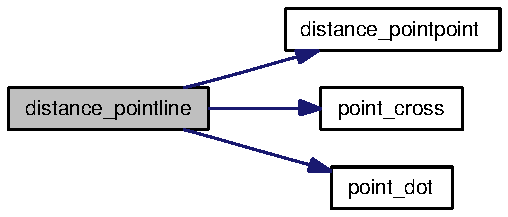
\includegraphics[width=140pt]{group__distance_g69a59a49134b784b0c8797e0e83e7c40_g69a59a49134b784b0c8797e0e83e7c40_cgraph}
\end{center}
\end{figure}


Here is the caller graph for this function:\begin{figure}[H]
\begin{center}
\leavevmode
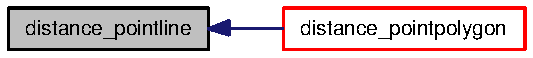
\includegraphics[width=146pt]{group__distance_g69a59a49134b784b0c8797e0e83e7c40_g69a59a49134b784b0c8797e0e83e7c40_icgraph}
\end{center}
\end{figure}
\hypertarget{group__distance_g3b2b03f846e6b587be683ec8b853e774_g3b2b03f846e6b587be683ec8b853e774}{
\index{distance@{distance}!distance_pointpoint@{distance\_\-pointpoint}}
\index{distance_pointpoint@{distance\_\-pointpoint}!distance@{distance}}
\subsubsection[distance\_\-pointpoint]{\setlength{\rightskip}{0pt plus 5cm}float distance\_\-pointpoint (\hyperlink{struct__point}{point} $\ast$ {\em a}, \hyperlink{struct__point}{point} $\ast$ {\em b})}}
\label{group__distance_g3b2b03f846e6b587be683ec8b853e774_g3b2b03f846e6b587be683ec8b853e774}


La funcion compara la distancia entre dos puntos la formula para esto es: $\sqrt{(x_2 - x_1)^2 + (y_2 - y_1)^2}$

\begin{Desc}
\item[Par\'{a}metros:]
\begin{description}
\item[\mbox{$\leftarrow$} {\em a}]Punto en 2 dimensiones \item[\mbox{$\leftarrow$} {\em b}]Punto en 2 dimensiones \end{description}
\end{Desc}
\begin{Desc}
\item[Devuelve:]La distancia entre los puntos \end{Desc}


Definici\'{o}n en la l\'{\i}nea 29 del archivo distance.c.

\begin{Code}\begin{verbatim}30 {
31     return sqrt(powf(a->x - b->x,2.0)+powf(a->y - b->y,2.0));
32 }
\end{verbatim}\end{Code}




Here is the caller graph for this function:\begin{figure}[H]
\begin{center}
\leavevmode
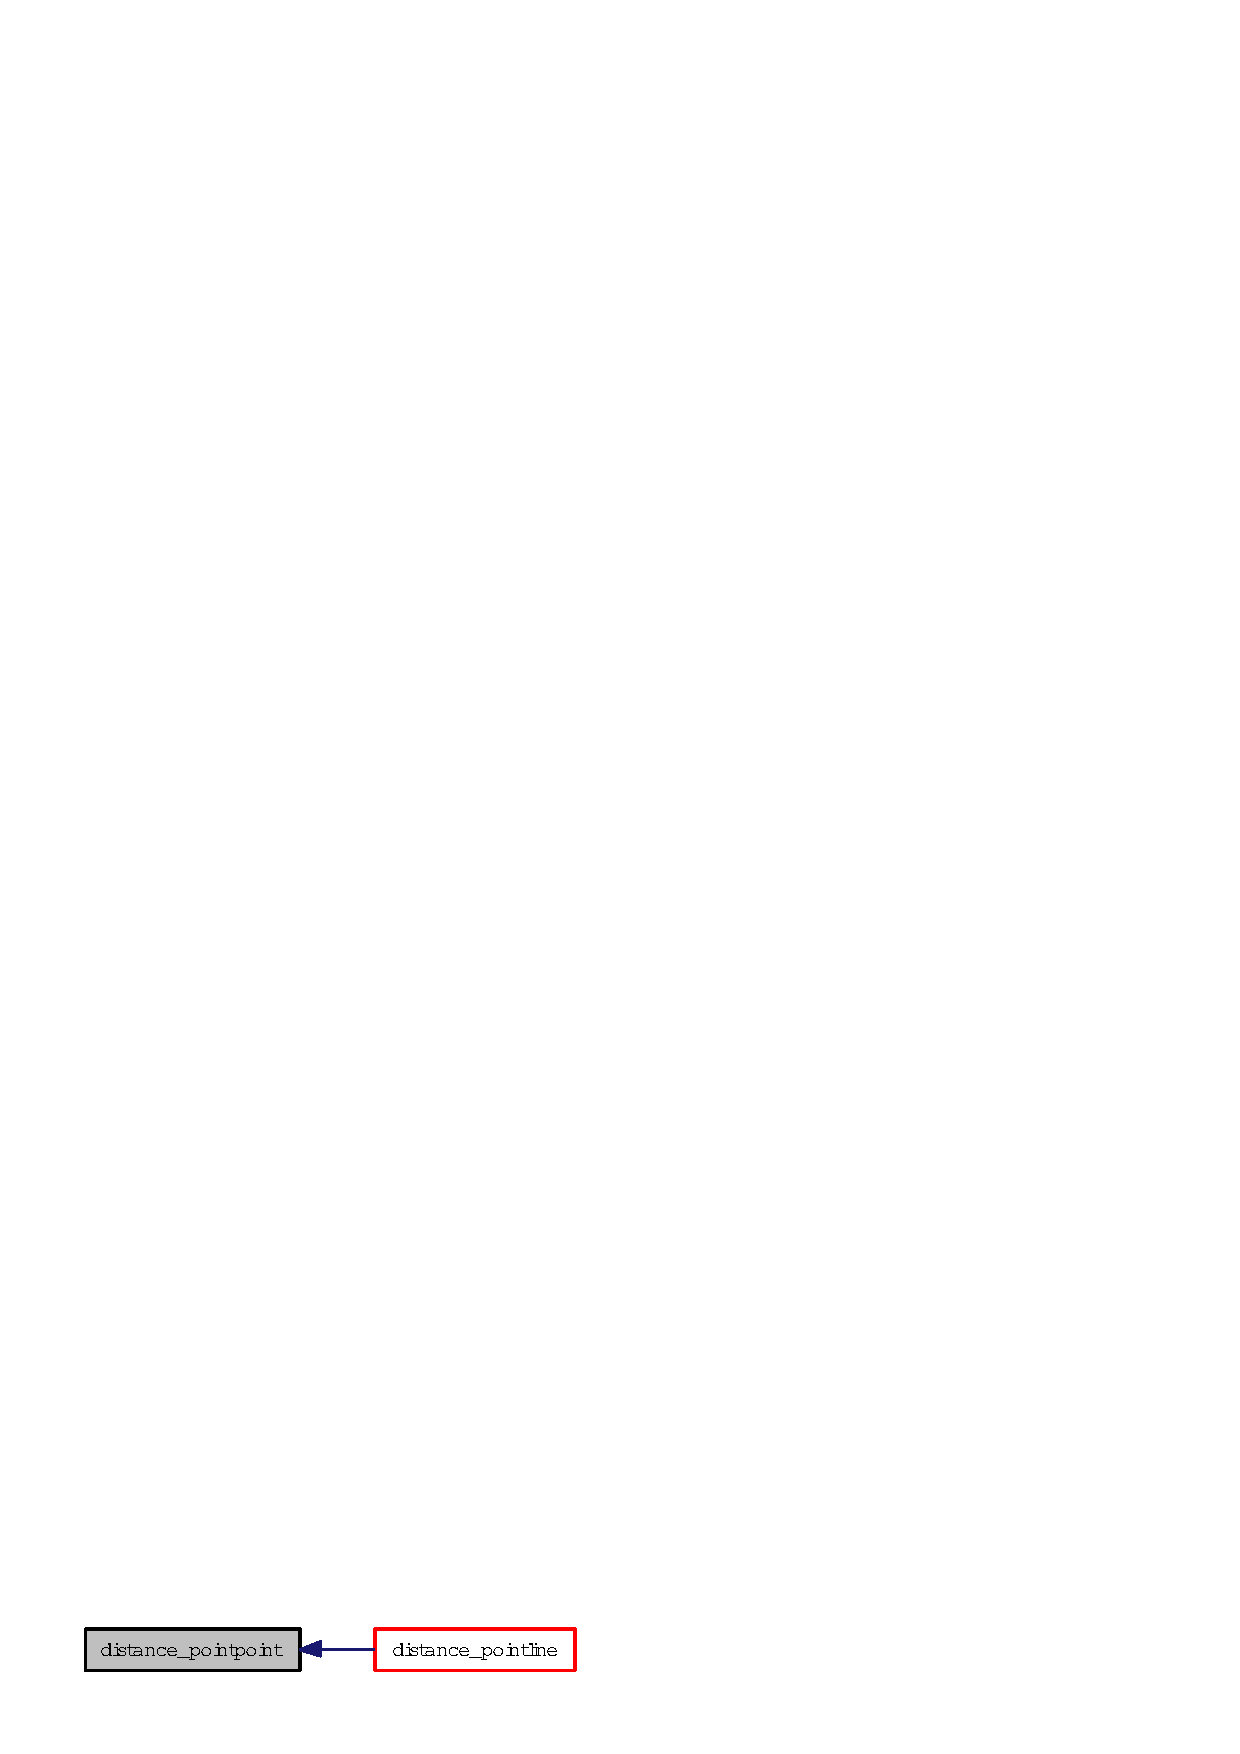
\includegraphics[width=140pt]{group__distance_g3b2b03f846e6b587be683ec8b853e774_g3b2b03f846e6b587be683ec8b853e774_icgraph}
\end{center}
\end{figure}
\hypertarget{group__distance_g25716e8d1c8abaf08903bbcd08b8d6e5_g25716e8d1c8abaf08903bbcd08b8d6e5}{
\index{distance@{distance}!distance_pointpolygon@{distance\_\-pointpolygon}}
\index{distance_pointpolygon@{distance\_\-pointpolygon}!distance@{distance}}
\subsubsection[distance\_\-pointpolygon]{\setlength{\rightskip}{0pt plus 5cm}float distance\_\-pointpolygon (\hyperlink{struct__point}{point} $\ast$ {\em f}, \hyperlink{struct__polygon}{polygon} $\ast$ {\em p}, \hyperlink{struct__line}{line} $\ast$ {\em ref})}}
\label{group__distance_g25716e8d1c8abaf08903bbcd08b8d6e5_g25716e8d1c8abaf08903bbcd08b8d6e5}


La funcion calcula la distancia entre un punto y el borde de un poligono simple, para esto calcula la distancia del punto contra todos los segmentos de linea que conforma el poligono y retorna la menor distancia, esta funcion no tiene consideracion si el punto esta adentro o afuera del poligono porque calcula la distancia al borde.

\begin{Desc}
\item[Par\'{a}metros:]
\begin{description}
\item[\mbox{$\leftarrow$} {\em f}]Punto en 2 dimensiones \item[\mbox{$\leftarrow$} {\em p}]Poligono simple \item[\mbox{$\rightarrow$} {\em ref}]Escribe en la memoria el segmento de recta que define la menor distancia entre el poligono y el punto, si la distancia fue tomada respecto a un punto extremo, entonces el segmento de recta es un punto, el extremo. \end{description}
\end{Desc}
\begin{Desc}
\item[Devuelve:]La distancia entre el punto y el poligono \end{Desc}


Definici\'{o}n en la l\'{\i}nea 87 del archivo distance.c.

\begin{Code}\begin{verbatim}88 {
89     int seg,i;
90     float min=FLT_MAX;
91 
92     for (i=0;i<p->nvertices;i++)
93     {
94         float d;
95         line l;
96 
97         l.v1=p->v[i];
98         l.v2=p->v[(i+1)%(p->nvertices)];
99         d=distance_pointline(f,&l,&seg);
100         if (i==0 || min>d)
101         {
102             min = d;
103             if (ref!=NULL)
104             {
105                 switch (seg)
106                 {
107                     case 0:
108                     ref->v1 = l.v1;
109                     ref->v2 = l.v2;
110                     break;
111                     case 1:
112                     ref->v1 = l.v1;
113                     ref->v2 = l.v1;
114                     break;
115                     case 2:
116                     ref->v1 = l.v2;
117                     ref->v2 = l.v2;
118                     break;
119                 }
120             }
121         }
122     }
123     return min;
124 }
\end{verbatim}\end{Code}




Gr\'{a}fico de llamadas para esta funci\'{o}n:\begin{figure}[H]
\begin{center}
\leavevmode
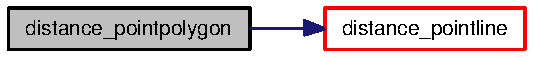
\includegraphics[width=146pt]{group__distance_g25716e8d1c8abaf08903bbcd08b8d6e5_g25716e8d1c8abaf08903bbcd08b8d6e5_cgraph}
\end{center}
\end{figure}


Here is the caller graph for this function:\begin{figure}[H]
\begin{center}
\leavevmode
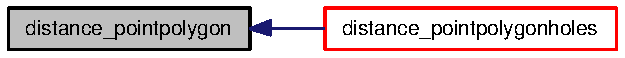
\includegraphics[width=168pt]{group__distance_g25716e8d1c8abaf08903bbcd08b8d6e5_g25716e8d1c8abaf08903bbcd08b8d6e5_icgraph}
\end{center}
\end{figure}
\hypertarget{group__distance_gc837f0084791f42936ade857a0cce3af_gc837f0084791f42936ade857a0cce3af}{
\index{distance@{distance}!distance_pointpolygonholes@{distance\_\-pointpolygonholes}}
\index{distance_pointpolygonholes@{distance\_\-pointpolygonholes}!distance@{distance}}
\subsubsection[distance\_\-pointpolygonholes]{\setlength{\rightskip}{0pt plus 5cm}float distance\_\-pointpolygonholes (\hyperlink{struct__point}{point} $\ast$ {\em f}, \hyperlink{struct__polygon__holes}{polygon\_\-holes} $\ast$ {\em p}, \hyperlink{struct__line}{line} $\ast$ {\em ref})}}
\label{group__distance_gc837f0084791f42936ade857a0cce3af_gc837f0084791f42936ade857a0cce3af}


La funcion calcula la distancia entre un punto y un poligono con huecos, para esto calcula la distancia del punto con el borde del poligono y posteriormente con cada uno de los huecos de este, seleccionado la distancia minima \begin{Desc}
\item[Par\'{a}metros:]
\begin{description}
\item[\mbox{$\leftarrow$} {\em f}]Punto en 2 dimensiones \item[\mbox{$\leftarrow$} {\em p}]Poligono con huecos \item[\mbox{$\rightarrow$} {\em ref}]Escribe en la memoria el segmento de recta que define la menor distancia entre el poligono y sus huecos con el punto, si la distancia fue tomada respecto a un punto extremo, entonces el segmento de recta es un punto, el extremo. \end{description}
\end{Desc}
\begin{Desc}
\item[Devuelve:]La distancia entre un punto y un poligono con huecos \end{Desc}


Definici\'{o}n en la l\'{\i}nea 139 del archivo distance.c.

\begin{Code}\begin{verbatim}140 {
141     int i;
142     float min;
143 
144     min = distance_pointpolygon(f,p->p,ref);
145     for (i=0;i<p->nholes;i++)
146     {
147         float min2;
148         line ref2;
149         min2 = distance_pointpolygon(f,&(p->h[i]),&ref2);
150         if (min2 < min)
151         {
152             min = min2;
153             if (ref!=NULL)
154             {
155                 ref->v1 = ref2.v1;
156                 ref->v2 = ref2.v2;
157             }
158         }
159     }
160     return min;
161 }
\end{verbatim}\end{Code}




Gr\'{a}fico de llamadas para esta funci\'{o}n:\begin{figure}[H]
\begin{center}
\leavevmode
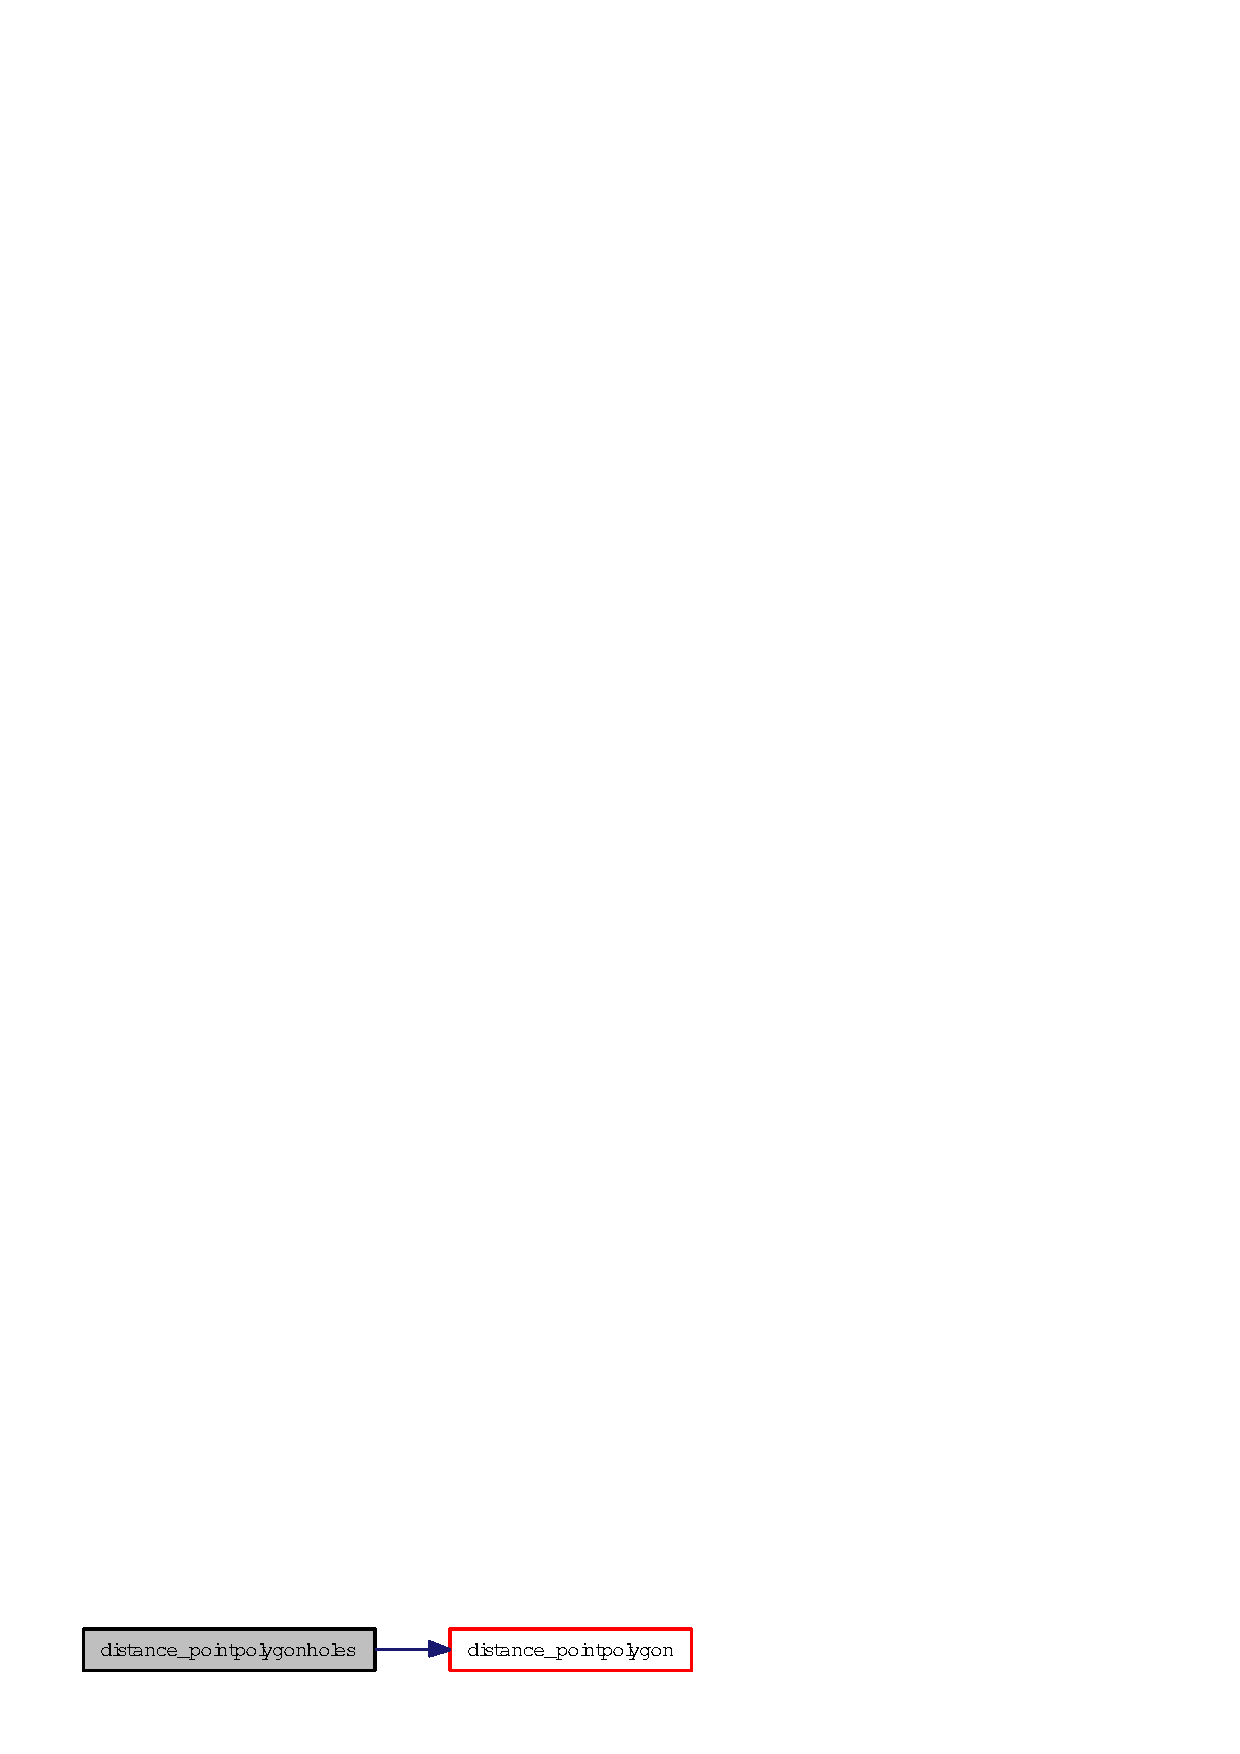
\includegraphics[width=168pt]{group__distance_gc837f0084791f42936ade857a0cce3af_gc837f0084791f42936ade857a0cce3af_cgraph}
\end{center}
\end{figure}


Here is the caller graph for this function:\begin{figure}[H]
\begin{center}
\leavevmode
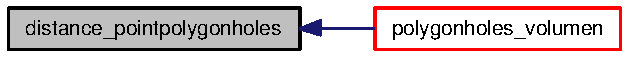
\includegraphics[width=169pt]{group__distance_gc837f0084791f42936ade857a0cce3af_gc837f0084791f42936ade857a0cce3af_icgraph}
\end{center}
\end{figure}

\hypertarget{group__geometry}{
\section{Geometria}
\label{group__geometry}\index{Geometria@{Geometria}}
}


\subsection{Descripci\'{o}n detallada}
Son los modelos y estructuras geometricas utilizadas para calcular las caracteristicas del problema, debido a que nesting esta fuertemente enlazado con poligonos, es necesario implementar el conjunto de objetos geometricos que lo manejen. 

\subsection*{Archivos}
\begin{CompactItemize}
\item 
archivo \hyperlink{line_8h}{line.h}
\item 
archivo \hyperlink{point_8h}{point.h}
\item 
archivo \hyperlink{polygon_8h}{polygon.h}
\item 
archivo \hyperlink{polygon__holes_8h}{polygon\_\-holes.h}
\item 
archivo \hyperlink{line_8c}{line.c}
\item 
archivo \hyperlink{point_8c}{point.c}
\item 
archivo \hyperlink{polygon_8c}{polygon.c}
\item 
archivo \hyperlink{polygon__holes_8c}{polygon\_\-holes.c}
\end{CompactItemize}
\subsection*{Clases}
\begin{CompactItemize}
\item 
struct \hyperlink{struct__line}{\_\-line}
\item 
struct \hyperlink{struct__point}{\_\-point}
\item 
struct \hyperlink{struct__polygon}{\_\-polygon}
\item 
struct \hyperlink{struct__polygon__holes}{\_\-polygon\_\-holes}
\end{CompactItemize}
\subsection*{Tipos definidos}
\begin{CompactItemize}
\item 
typedef \hyperlink{struct__line}{\_\-line} \hyperlink{group__geometry_gbb4d6a1464226fe9b7c0d80348e5eb98_gbb4d6a1464226fe9b7c0d80348e5eb98}{line}
\item 
typedef \hyperlink{struct__point}{\_\-point} \hyperlink{group__geometry_g37e9de632d1eb76ff7dcd3d8172add7d_g37e9de632d1eb76ff7dcd3d8172add7d}{point}
\item 
typedef \hyperlink{struct__polygon}{\_\-polygon} \hyperlink{group__geometry_g9169f21a34d344b356c44948943e99cc_g9169f21a34d344b356c44948943e99cc}{polygon}
\item 
typedef \hyperlink{struct__polygon__holes}{\_\-polygon\_\-holes} \hyperlink{group__geometry_g1137695e6ed0a9b25685f8bf3ccdb45f_g1137695e6ed0a9b25685f8bf3ccdb45f}{polygon\_\-holes}
\end{CompactItemize}
\subsection*{Funciones}
\begin{CompactItemize}
\item 
bool \hyperlink{group__geometry_g95f804c79e71c1ca62453b6f0123e307_g95f804c79e71c1ca62453b6f0123e307}{line\_\-intersection} (\hyperlink{struct__line}{line} $\ast$l1, \hyperlink{struct__line}{line} $\ast$l2)
\item 
bool \hyperlink{group__geometry_ga27fbafb04a36a60af7bd5cafbdfd412_ga27fbafb04a36a60af7bd5cafbdfd412}{line\_\-equal} (\hyperlink{struct__line}{line} $\ast$l1, \hyperlink{struct__line}{line} $\ast$l2)
\item 
bool \hyperlink{group__geometry_g68d4dad9b8e742b0d63affc853f80391_g68d4dad9b8e742b0d63affc853f80391}{line\_\-ispoint} (\hyperlink{struct__line}{line} $\ast$l1)
\item 
float \hyperlink{group__geometry_ga7ae8d919209fea43e8a61215398bbbe_ga7ae8d919209fea43e8a61215398bbbe}{point\_\-dot} (\hyperlink{struct__point}{point} $\ast$a, \hyperlink{struct__point}{point} $\ast$b, \hyperlink{struct__point}{point} $\ast$c)
\item 
float \hyperlink{group__geometry_gb97527165a510655ee37cd3ccfa8d932_gb97527165a510655ee37cd3ccfa8d932}{point\_\-cross} (\hyperlink{struct__point}{point} $\ast$a, \hyperlink{struct__point}{point} $\ast$b, \hyperlink{struct__point}{point} $\ast$c)
\item 
float \hyperlink{group__geometry_gcfbc9e7772d80361768bc0b65cebbca1_gcfbc9e7772d80361768bc0b65cebbca1}{polygon\_\-area} (\hyperlink{struct__polygon}{polygon} $\ast$p)
\item 
bool \hyperlink{group__geometry_geab0a1d6da7c44ae49494958bb885504_geab0a1d6da7c44ae49494958bb885504}{polygon\_\-pointin} (\hyperlink{struct__polygon}{polygon} $\ast$p, \hyperlink{struct__point}{point} $\ast$f)
\item 
bool \hyperlink{group__geometry_g2be6101a257ea8896e61e93d14b22b89_g2be6101a257ea8896e61e93d14b22b89}{polygon\_\-overlapping} (\hyperlink{struct__polygon}{polygon} $\ast$p, \hyperlink{struct__polygon}{polygon} $\ast$q)
\item 
void \hyperlink{group__geometry_g95276abee7240f116afaf80a3e1f23c4_g95276abee7240f116afaf80a3e1f23c4}{polygon\_\-rotate} (\hyperlink{struct__polygon}{polygon} $\ast$p, float t)
\item 
void \hyperlink{group__geometry_g137ef6f552a0a04c5ae0493690088f3f_g137ef6f552a0a04c5ae0493690088f3f}{polygon\_\-minbox} (\hyperlink{struct__polygon}{polygon} $\ast$p, float $\ast$minx, float $\ast$miny, float $\ast$maxx, float $\ast$maxy)
\item 
void \hyperlink{group__geometry_g7538c2bf0d1e8acc0cfc055b6bf3a96b_g7538c2bf0d1e8acc0cfc055b6bf3a96b}{polygon\_\-translate} (\hyperlink{struct__polygon}{polygon} $\ast$p, float x, float y)
\item 
float \hyperlink{group__geometry_g380cdcfa6caf51828c8d06f4518a4084_g380cdcfa6caf51828c8d06f4518a4084}{polygonholes\_\-area} (\hyperlink{struct__polygon__holes}{polygon\_\-holes} $\ast$p)
\item 
float \hyperlink{group__geometry_g7cf8b3f8c76179bb936754bbbf510999_g7cf8b3f8c76179bb936754bbbf510999}{polygonholes\_\-volumen} (\hyperlink{struct__polygon__holes}{polygon\_\-holes} $\ast$p)
\item 
bool \hyperlink{group__geometry_g35a6dd45f6d0cbed26ef8a69ed34a2e9_g35a6dd45f6d0cbed26ef8a69ed34a2e9}{polygonholes\_\-pointin} (\hyperlink{struct__polygon__holes}{polygon\_\-holes} $\ast$p, \hyperlink{struct__point}{point} $\ast$f)
\item 
bool \hyperlink{group__geometry_g496bae87588cb5710ced80f713da98ad_g496bae87588cb5710ced80f713da98ad}{polygonholes\_\-polygonin} (\hyperlink{struct__polygon__holes}{polygon\_\-holes} $\ast$p, \hyperlink{struct__polygon}{polygon} $\ast$q)
\item 
bool \hyperlink{group__geometry_g139317720b027c782db9424256ba2c2d_g139317720b027c782db9424256ba2c2d}{polygonholes\_\-pointinhole} (\hyperlink{struct__polygon__holes}{polygon\_\-holes} $\ast$p, \hyperlink{struct__point}{point} $\ast$f)
\item 
\hyperlink{struct__point}{point} \hyperlink{group__geometry_ge39fef354e4411678ec081c197b29825_ge39fef354e4411678ec081c197b29825}{polygon\_\-center} (\hyperlink{struct__polygon}{polygon} $\ast$p)
\end{CompactItemize}


\subsection{Documentaci\'{o}n de los tipos definidos}
\hypertarget{group__geometry_gbb4d6a1464226fe9b7c0d80348e5eb98_gbb4d6a1464226fe9b7c0d80348e5eb98}{
\index{geometry@{geometry}!line@{line}}
\index{line@{line}!geometry@{geometry}}
\subsubsection[line]{\setlength{\rightskip}{0pt plus 5cm}typedef struct \hyperlink{struct__line}{\_\-line} \hyperlink{struct__line}{line}}}
\label{group__geometry_gbb4d6a1464226fe9b7c0d80348e5eb98_gbb4d6a1464226fe9b7c0d80348e5eb98}




Definici\'{o}n en la l\'{\i}nea 21 del archivo line.h.\hypertarget{group__geometry_g37e9de632d1eb76ff7dcd3d8172add7d_g37e9de632d1eb76ff7dcd3d8172add7d}{
\index{geometry@{geometry}!point@{point}}
\index{point@{point}!geometry@{geometry}}
\subsubsection[point]{\setlength{\rightskip}{0pt plus 5cm}typedef struct \hyperlink{struct__point}{\_\-point} \hyperlink{struct__point}{point}}}
\label{group__geometry_g37e9de632d1eb76ff7dcd3d8172add7d_g37e9de632d1eb76ff7dcd3d8172add7d}




Definici\'{o}n en la l\'{\i}nea 17 del archivo point.h.\hypertarget{group__geometry_g9169f21a34d344b356c44948943e99cc_g9169f21a34d344b356c44948943e99cc}{
\index{geometry@{geometry}!polygon@{polygon}}
\index{polygon@{polygon}!geometry@{geometry}}
\subsubsection[polygon]{\setlength{\rightskip}{0pt plus 5cm}typedef struct \hyperlink{struct__polygon}{\_\-polygon} \hyperlink{struct__polygon}{polygon}}}
\label{group__geometry_g9169f21a34d344b356c44948943e99cc_g9169f21a34d344b356c44948943e99cc}




Definici\'{o}n en la l\'{\i}nea 24 del archivo polygon.h.\hypertarget{group__geometry_g1137695e6ed0a9b25685f8bf3ccdb45f_g1137695e6ed0a9b25685f8bf3ccdb45f}{
\index{geometry@{geometry}!polygon_holes@{polygon\_\-holes}}
\index{polygon_holes@{polygon\_\-holes}!geometry@{geometry}}
\subsubsection[polygon\_\-holes]{\setlength{\rightskip}{0pt plus 5cm}typedef struct \hyperlink{struct__polygon__holes}{\_\-polygon\_\-holes} \hyperlink{struct__polygon__holes}{polygon\_\-holes}}}
\label{group__geometry_g1137695e6ed0a9b25685f8bf3ccdb45f_g1137695e6ed0a9b25685f8bf3ccdb45f}




Definici\'{o}n en la l\'{\i}nea 24 del archivo polygon\_\-holes.h.

\subsection{Documentaci\'{o}n de las funciones}
\hypertarget{group__geometry_ga27fbafb04a36a60af7bd5cafbdfd412_ga27fbafb04a36a60af7bd5cafbdfd412}{
\index{geometry@{geometry}!line_equal@{line\_\-equal}}
\index{line_equal@{line\_\-equal}!geometry@{geometry}}
\subsubsection[line\_\-equal]{\setlength{\rightskip}{0pt plus 5cm}bool line\_\-equal (\hyperlink{struct__line}{line} $\ast$ {\em l1}, \hyperlink{struct__line}{line} $\ast$ {\em l2})}}
\label{group__geometry_ga27fbafb04a36a60af7bd5cafbdfd412_ga27fbafb04a36a60af7bd5cafbdfd412}


Compara dos segmentos de linea, en este caso el orden de los extremos importa en la operacion

\begin{Desc}
\item[Par\'{a}metros:]
\begin{description}
\item[\mbox{$\leftarrow$} {\em l1}]Linea en 2 dimensiones \item[\mbox{$\leftarrow$} {\em l2}]Linea en 2 dimensiones \end{description}
\end{Desc}
\begin{Desc}
\item[Devuelve:]Verdadero si los segmentos de recta son iguales, falso en caso contrario \end{Desc}


Definici\'{o}n en la l\'{\i}nea 109 del archivo line.c.

\begin{Code}\begin{verbatim}110 {
111     return (l1->v1.x == l2->v1.x &&
112             l1->v1.y == l2->v1.y &&
113             l1->v2.x == l2->v2.x &&
114             l1->v2.y == l2->v2.y
115            ) ? true : false;
116 }
\end{verbatim}\end{Code}




Here is the caller graph for this function:\begin{figure}[H]
\begin{center}
\leavevmode
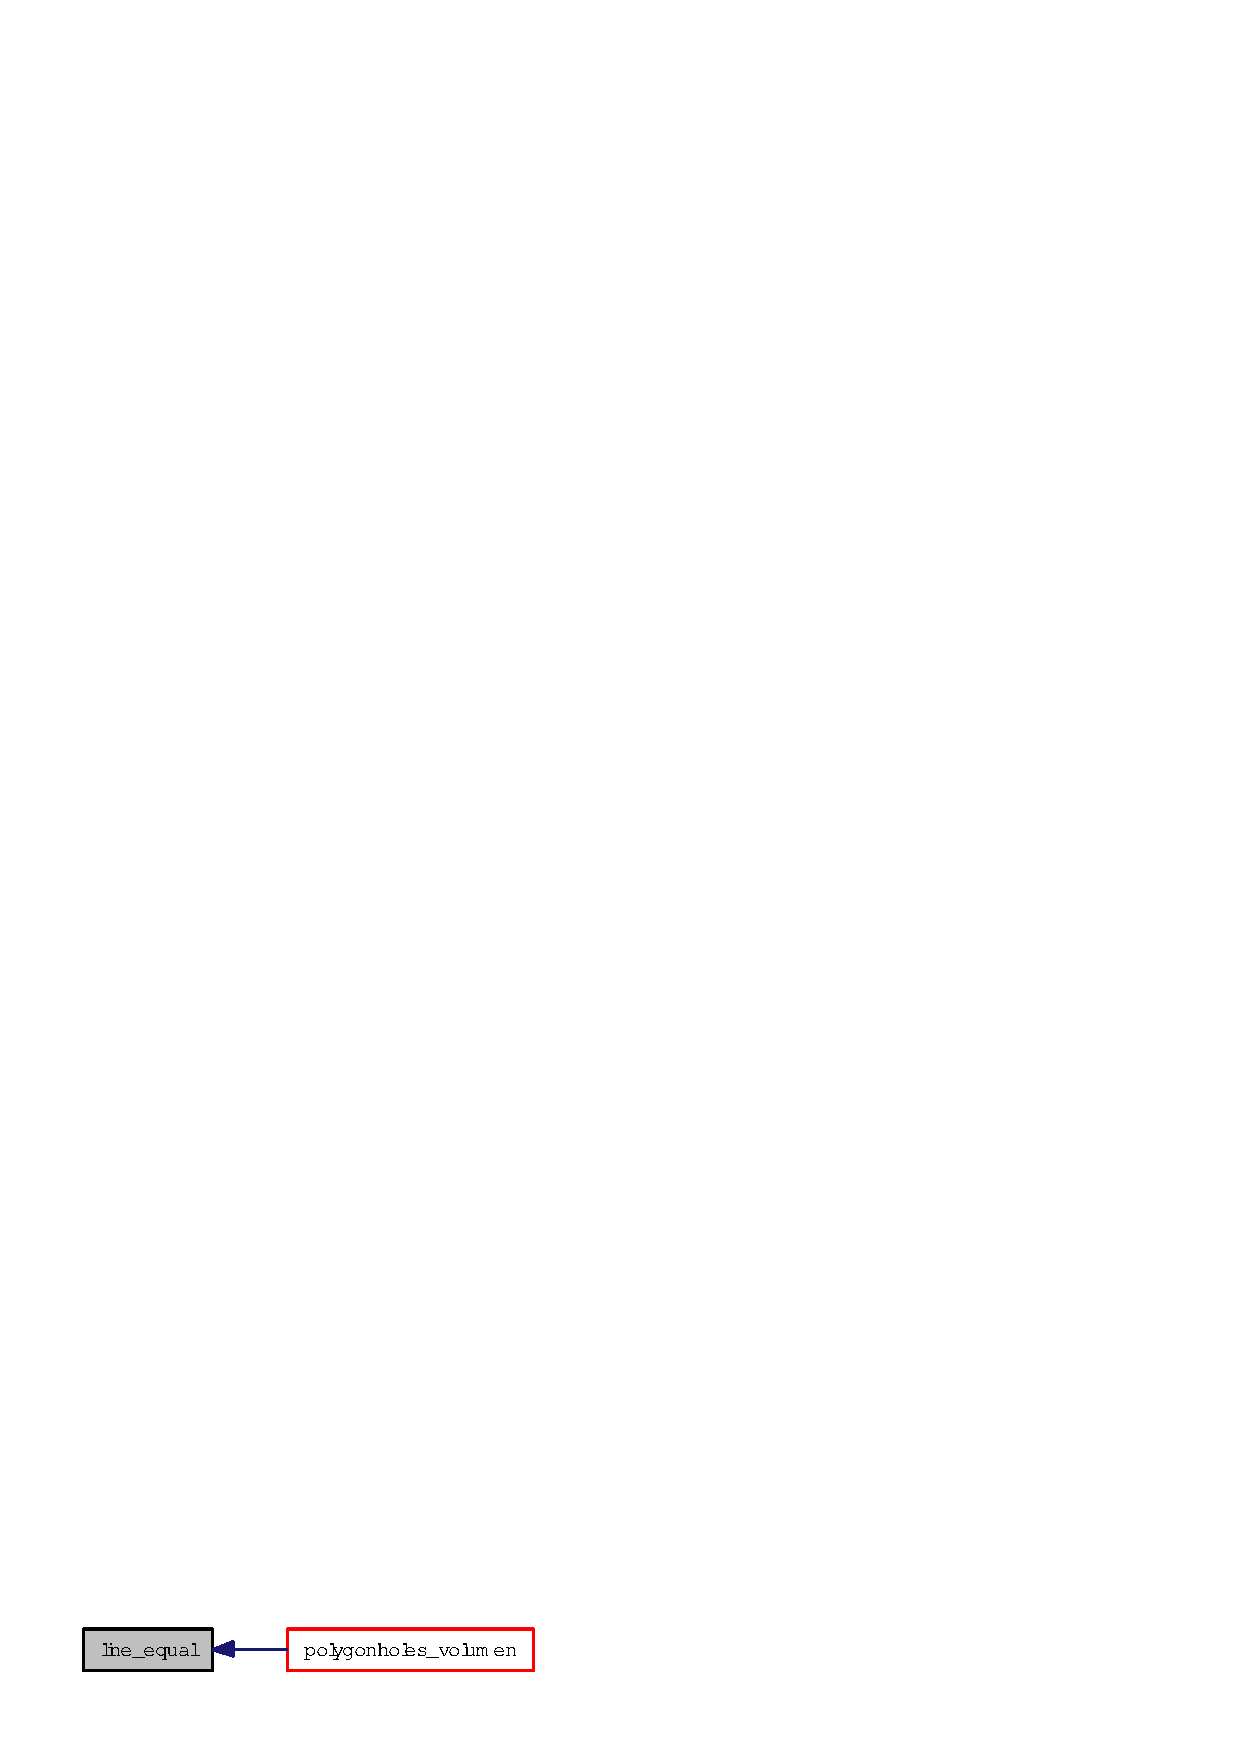
\includegraphics[width=130pt]{group__geometry_ga27fbafb04a36a60af7bd5cafbdfd412_ga27fbafb04a36a60af7bd5cafbdfd412_icgraph}
\end{center}
\end{figure}
\hypertarget{group__geometry_g95f804c79e71c1ca62453b6f0123e307_g95f804c79e71c1ca62453b6f0123e307}{
\index{geometry@{geometry}!line_intersection@{line\_\-intersection}}
\index{line_intersection@{line\_\-intersection}!geometry@{geometry}}
\subsubsection[line\_\-intersection]{\setlength{\rightskip}{0pt plus 5cm}bool line\_\-intersection (\hyperlink{struct__line}{line} $\ast$ {\em l1}, \hyperlink{struct__line}{line} $\ast$ {\em l2})}}
\label{group__geometry_g95f804c79e71c1ca62453b6f0123e307_g95f804c79e71c1ca62453b6f0123e307}


Identifica si dos lineas se intersectan, el algoritmo utilizado fue sacado del libro de Graphics Gems del Articulo Faster Line Segment Intersection

\begin{Desc}
\item[Par\'{a}metros:]
\begin{description}
\item[\mbox{$\leftarrow$} {\em l1}]Linea en 2 dimensiones \item[\mbox{$\leftarrow$} {\em l2}]Linea en 2 dimensiones \end{description}
\end{Desc}
\begin{Desc}
\item[Devuelve:]Un valor booleano que es verdadero si las lineas se intersectan y falso en caso contrario \end{Desc}


Definici\'{o}n en la l\'{\i}nea 22 del archivo line.c.

\begin{Code}\begin{verbatim}23 {
24     float x1,y1,x2,y2,x3,y3,x4,y4;
25     float Ax,Bx,Cx,Ay,By,Cy;
26     float x1lo,x1hi,y1lo,y1hi;
27     float d,e,f;
28 
29     x1 = l1->v1.x;
30     y1 = l1->v1.y;
31 
32     x2 = l1->v2.x;
33     y2 = l1->v2.y;
34 
35     x3 = l2->v1.x;
36     y3 = l2->v1.y;
37 
38     x4 = l2->v2.x;
39     y4 = l2->v2.y;
40 
41     Ax = x2 - x1;
42     Bx = x3 - x4;
43 
44     if (Ax < 0){
45         x1lo=x2;
46         x1hi=x1;
47     } else {
48         x1hi=x2;
49         x1lo=x1;
50     }
51 
52     if (Bx > 0){
53             if (x1hi < x4 || x2 < x1lo) return false;
54     } else {
55             if (x1hi < x3 || x4 < x1lo) return false;
56     }
57 
58     Ay = y2 - y1;
59     By = y3 - y4;
60 
61     if (Ay < 0){
62             y1lo = y2;
63             y1hi = y1;
64     } else {
65             y1hi = y2;
66             y1lo = y1;
67     }
68 
69     if (By > 0){
70             if (y1hi < y4 || y3 < y1lo) return false;
71     } else {
72             if (y1hi < y3 || y4 < y1lo) return false;
73     }
74 
75     Cx = x1 - x3;
76     Cy = y1 - y3;
77 
78     d = By*Cx - Bx*Cy;
79     f = Ay*Bx - Ax*By;
80 
81     if (f>0){
82             if (d<0 || d>f) return false;
83     } else {
84             if (d>0 || d<f) return false;
85     }
86 
87     e = Ax*Cy - Ay*Cx;
88 
89     if (f>0){
90             if (e<0 || e>f) return false;
91     } else {
92             if (e>0 || e<f) return false;
93     }
94 
95     if (f==0) return false;
96 
97     return true;
98 }
\end{verbatim}\end{Code}




Here is the caller graph for this function:\begin{figure}[H]
\begin{center}
\leavevmode
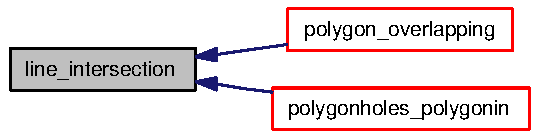
\includegraphics[width=147pt]{group__geometry_g95f804c79e71c1ca62453b6f0123e307_g95f804c79e71c1ca62453b6f0123e307_icgraph}
\end{center}
\end{figure}
\hypertarget{group__geometry_g68d4dad9b8e742b0d63affc853f80391_g68d4dad9b8e742b0d63affc853f80391}{
\index{geometry@{geometry}!line_ispoint@{line\_\-ispoint}}
\index{line_ispoint@{line\_\-ispoint}!geometry@{geometry}}
\subsubsection[line\_\-ispoint]{\setlength{\rightskip}{0pt plus 5cm}bool line\_\-ispoint (\hyperlink{struct__line}{line} $\ast$ {\em l})}}
\label{group__geometry_g68d4dad9b8e742b0d63affc853f80391_g68d4dad9b8e742b0d63affc853f80391}


Identifica si un segmento de recta es en realidad un unico punto, esto lo hace comprobando los puntos extremos del segmento de recta, si los extremos son iguales entonces se puede definir este segmento de recta como una linea

\begin{Desc}
\item[Par\'{a}metros:]
\begin{description}
\item[\mbox{$\leftarrow$} {\em l}]Linea en 2 dimensiones \end{description}
\end{Desc}
\begin{Desc}
\item[Devuelve:]Verdadero si la linea es un punto, falso en caso contrario. \end{Desc}


Definici\'{o}n en la l\'{\i}nea 128 del archivo line.c.

\begin{Code}\begin{verbatim}129 {
130     return (l->v1.x == l->v2.x && l->v1.y == l->v2.y) ? true : false;
131 }
\end{verbatim}\end{Code}




Here is the caller graph for this function:\begin{figure}[H]
\begin{center}
\leavevmode
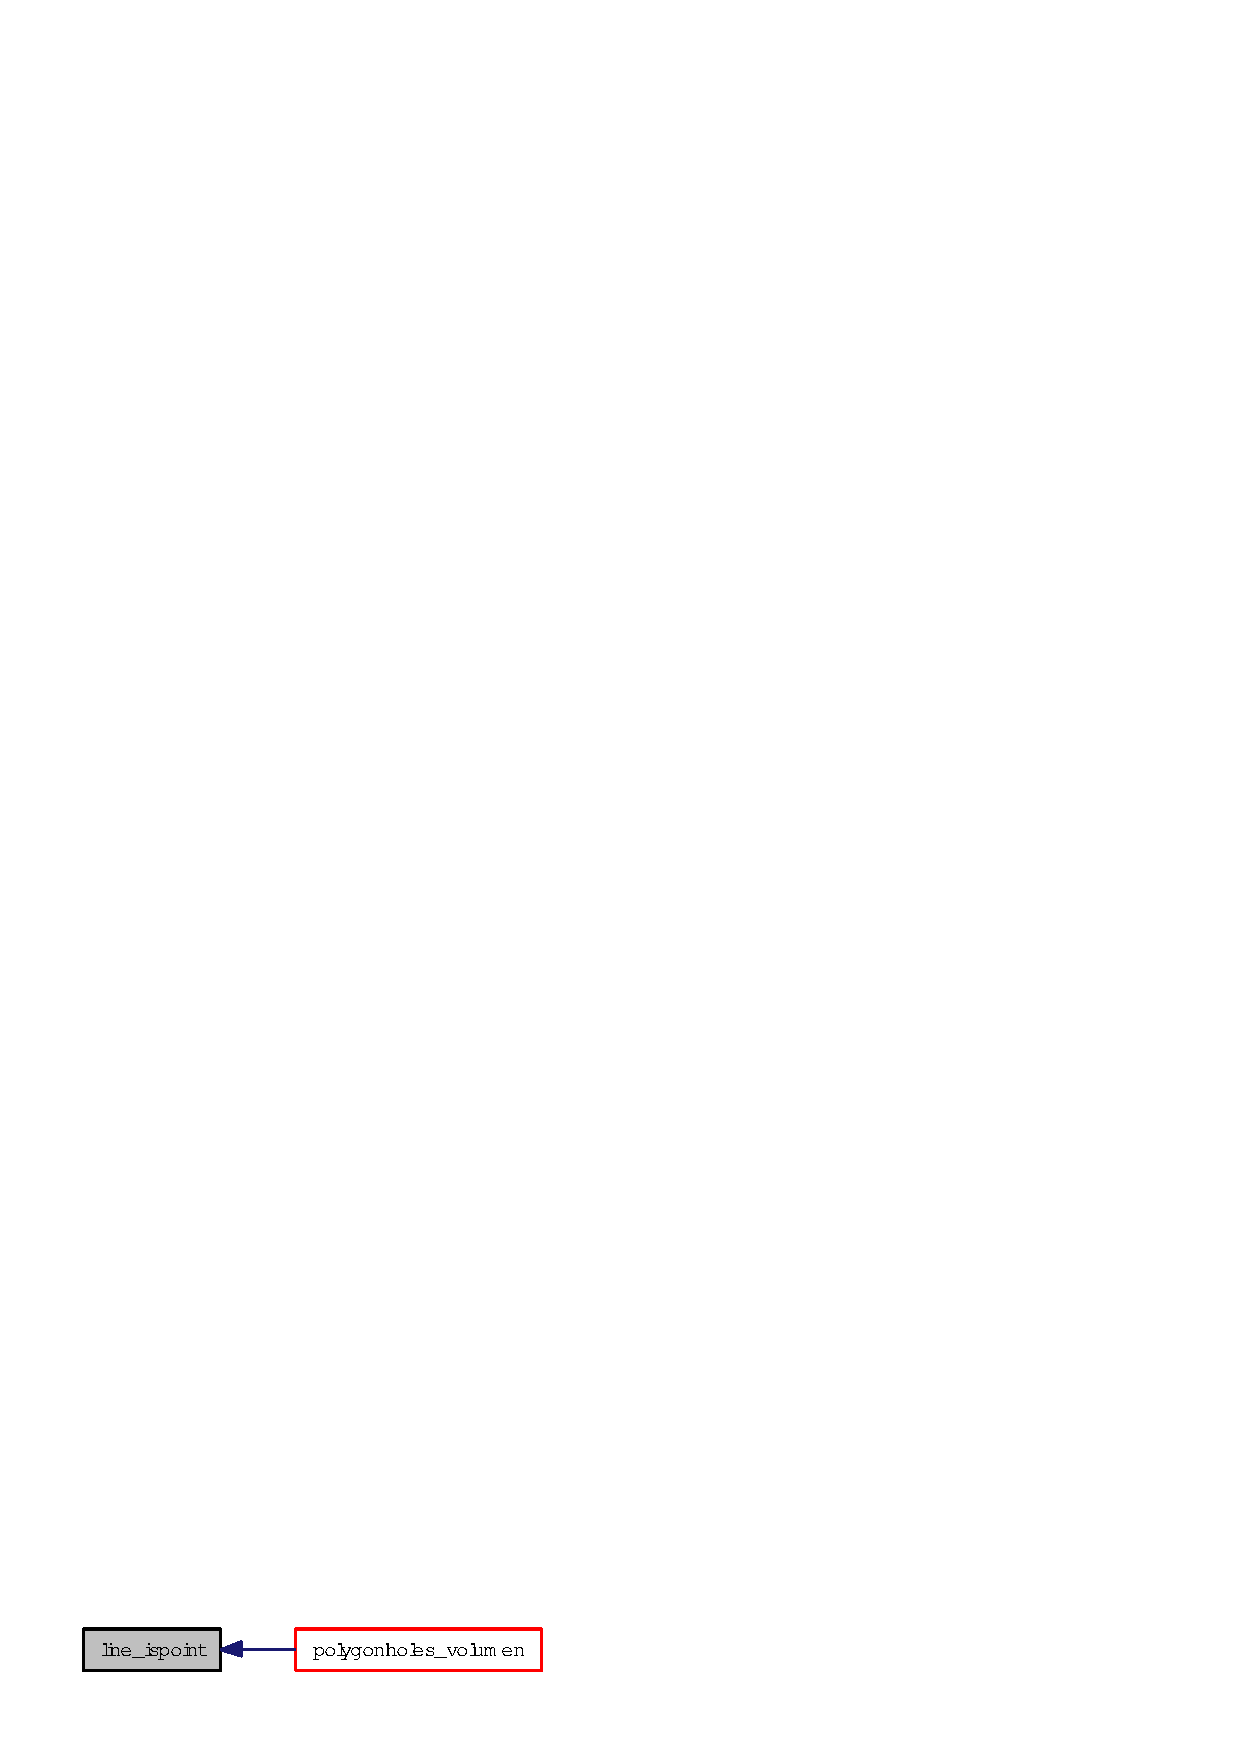
\includegraphics[width=132pt]{group__geometry_g68d4dad9b8e742b0d63affc853f80391_g68d4dad9b8e742b0d63affc853f80391_icgraph}
\end{center}
\end{figure}
\hypertarget{group__geometry_gb97527165a510655ee37cd3ccfa8d932_gb97527165a510655ee37cd3ccfa8d932}{
\index{geometry@{geometry}!point_cross@{point\_\-cross}}
\index{point_cross@{point\_\-cross}!geometry@{geometry}}
\subsubsection[point\_\-cross]{\setlength{\rightskip}{0pt plus 5cm}float point\_\-cross (\hyperlink{struct__point}{point} $\ast$ {\em a}, \hyperlink{struct__point}{point} $\ast$ {\em b}, \hyperlink{struct__point}{point} $\ast$ {\em c})}}
\label{group__geometry_gb97527165a510655ee37cd3ccfa8d932_gb97527165a510655ee37cd3ccfa8d932}


Calcula el producto cruz entro los punto a, b y c. Aunque esta funcion matematicamente esta definida en los vectores y no en los puntos, podemos relacionar un punto como el vector que hay desde el origen del plano hasta las coordenadas de este y asi calculamos el producto cruz.

\begin{Desc}
\item[Par\'{a}metros:]
\begin{description}
\item[\mbox{$\leftarrow$} {\em a}]Punto en 2 dimensiones \item[\mbox{$\leftarrow$} {\em b}]Punto en 2 dimensiones \item[\mbox{$\leftarrow$} {\em c}]Punto en 2 dimensiones \end{description}
\end{Desc}
\begin{Desc}
\item[Devuelve:]El producto cruz \end{Desc}


Definici\'{o}n en la l\'{\i}nea 38 del archivo point.c.

\begin{Code}\begin{verbatim}39 {
40     return ((b->x - a->x)*(c->y - a->y)) - ((b->y - a->y)*(c->x - a->x));
41 }
\end{verbatim}\end{Code}




Here is the caller graph for this function:\begin{figure}[H]
\begin{center}
\leavevmode
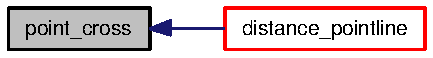
\includegraphics[width=122pt]{group__geometry_gb97527165a510655ee37cd3ccfa8d932_gb97527165a510655ee37cd3ccfa8d932_icgraph}
\end{center}
\end{figure}
\hypertarget{group__geometry_ga7ae8d919209fea43e8a61215398bbbe_ga7ae8d919209fea43e8a61215398bbbe}{
\index{geometry@{geometry}!point_dot@{point\_\-dot}}
\index{point_dot@{point\_\-dot}!geometry@{geometry}}
\subsubsection[point\_\-dot]{\setlength{\rightskip}{0pt plus 5cm}float point\_\-dot (\hyperlink{struct__point}{point} $\ast$ {\em a}, \hyperlink{struct__point}{point} $\ast$ {\em b}, \hyperlink{struct__point}{point} $\ast$ {\em c})}}
\label{group__geometry_ga7ae8d919209fea43e8a61215398bbbe_ga7ae8d919209fea43e8a61215398bbbe}


Calcula el producto punto entre los puntos a, b y c. Aunque esta funcion matematicamente esta definida en los vectores y no en los puntos, podemos relacionar un punto como el vector que hay desde el origen del plano hasta las coordenadas de este y asi calculamos el producto punto.

\begin{Desc}
\item[Par\'{a}metros:]
\begin{description}
\item[\mbox{$\leftarrow$} {\em a}]Punto en 2 dimensiones \item[\mbox{$\leftarrow$} {\em b}]Punto en 2 dimensiones \item[\mbox{$\leftarrow$} {\em c}]Punto en 2 dimensiones \end{description}
\end{Desc}
\begin{Desc}
\item[Devuelve:]El producto punto \end{Desc}


Definici\'{o}n en la l\'{\i}nea 21 del archivo point.c.

\begin{Code}\begin{verbatim}22 {
23     return ((b->x - a->x) * (c->x - b->x)) + ((b->y - a->y) * (c->y - b->y));
24 }
\end{verbatim}\end{Code}




Here is the caller graph for this function:\begin{figure}[H]
\begin{center}
\leavevmode
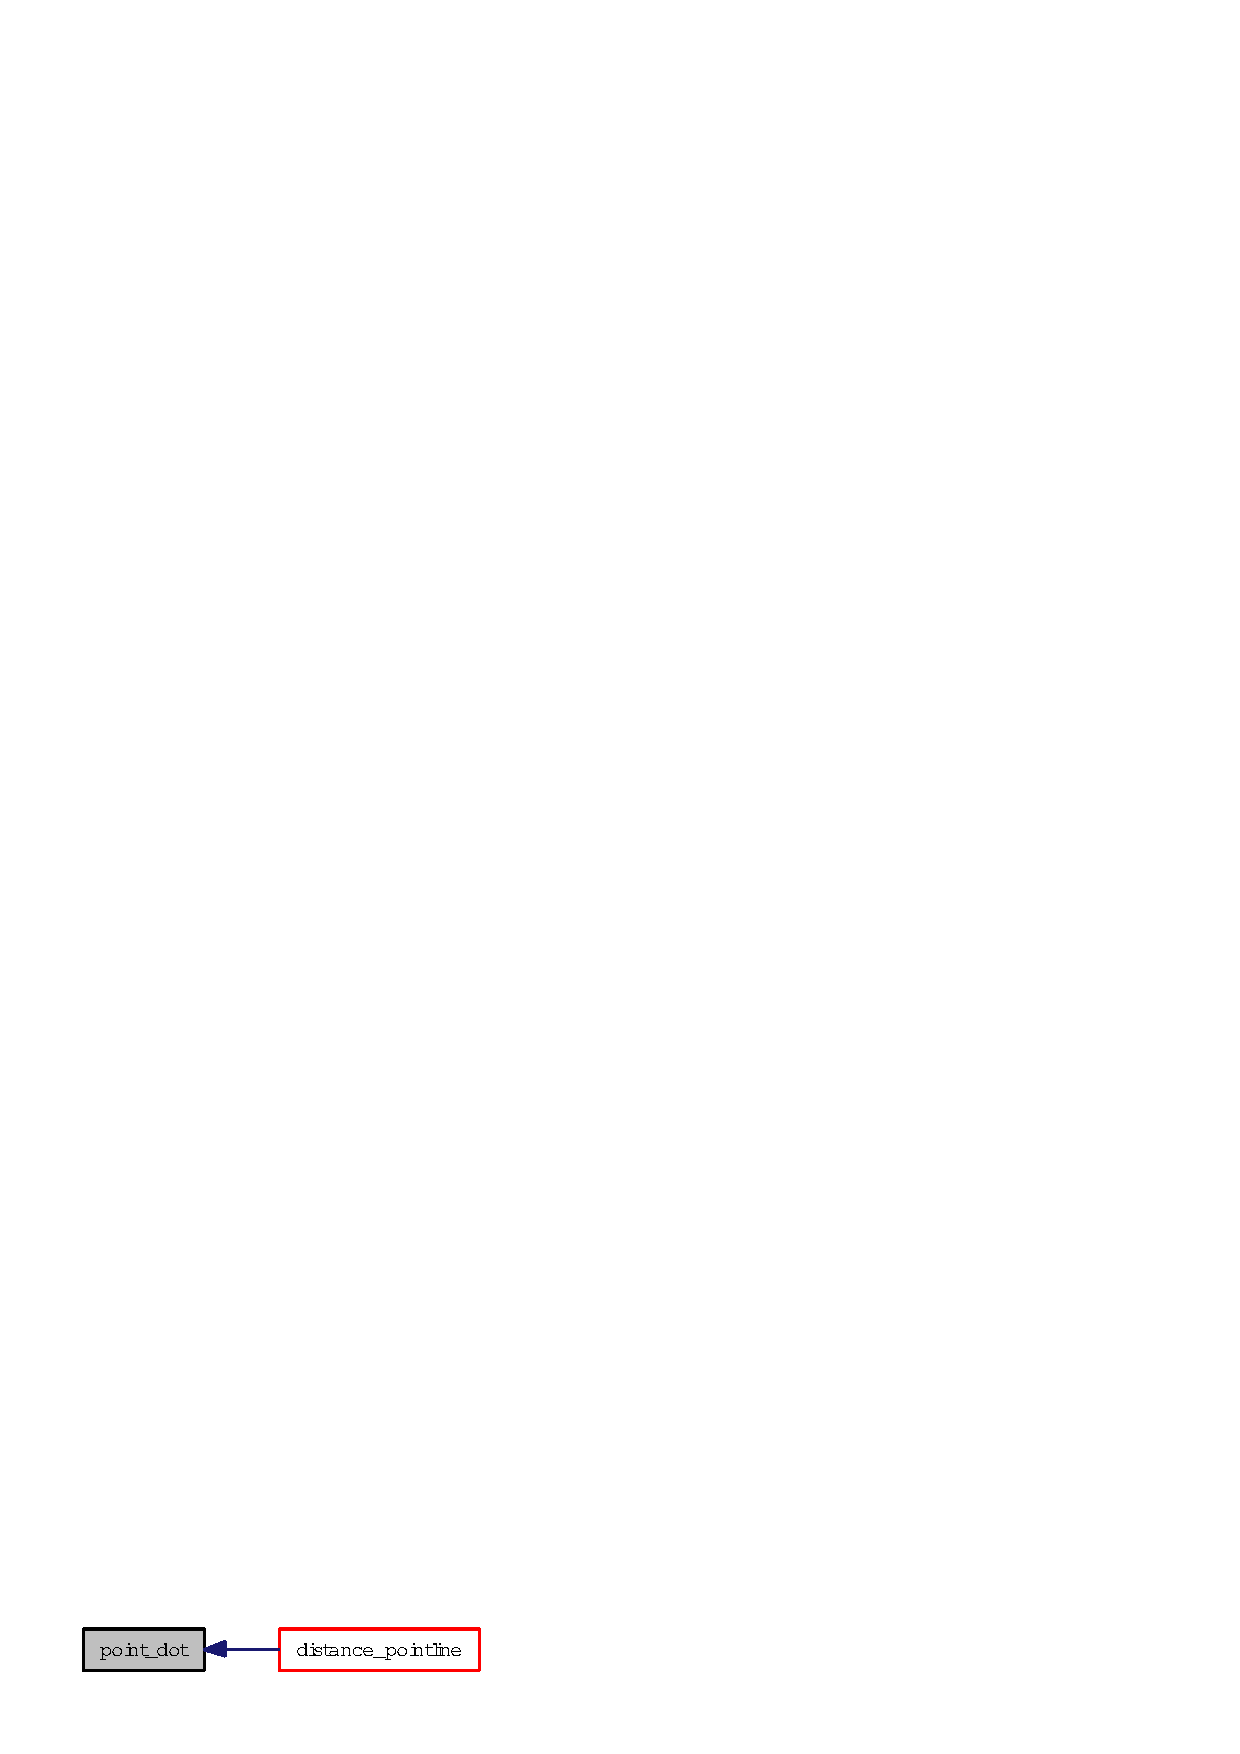
\includegraphics[width=117pt]{group__geometry_ga7ae8d919209fea43e8a61215398bbbe_ga7ae8d919209fea43e8a61215398bbbe_icgraph}
\end{center}
\end{figure}
\hypertarget{group__geometry_gcfbc9e7772d80361768bc0b65cebbca1_gcfbc9e7772d80361768bc0b65cebbca1}{
\index{geometry@{geometry}!polygon_area@{polygon\_\-area}}
\index{polygon_area@{polygon\_\-area}!geometry@{geometry}}
\subsubsection[polygon\_\-area]{\setlength{\rightskip}{0pt plus 5cm}float polygon\_\-area (\hyperlink{struct__polygon}{polygon} $\ast$ {\em p})}}
\label{group__geometry_gcfbc9e7772d80361768bc0b65cebbca1_gcfbc9e7772d80361768bc0b65cebbca1}


Esta funcion calcula el area de un poligono simple, el algoritmo fue tomado de Graphic Gems II, del articulo The Area of a Simple Polygon.

\begin{Desc}
\item[Par\'{a}metros:]
\begin{description}
\item[\mbox{$\leftarrow$} {\em p}]Poligono simple \end{description}
\end{Desc}
\begin{Desc}
\item[Devuelve:]El area del poligono \end{Desc}


Definici\'{o}n en la l\'{\i}nea 20 del archivo polygon.c.

\begin{Code}\begin{verbatim}21 {
22     unsigned int i;
23     float area = 0;
24     for (i=0;i<p->nvertices;i++)
25     {
26         area += p->v[i].x * p->v[(i + 1) % p->nvertices].y;
27         area -= p->v[i].y * p->v[(i + 1) % p->nvertices].x;
28     }
29     area /= 2;
30 
31     return(area < 0 ? -area : area);
32 }
\end{verbatim}\end{Code}




Here is the caller graph for this function:\begin{figure}[H]
\begin{center}
\leavevmode
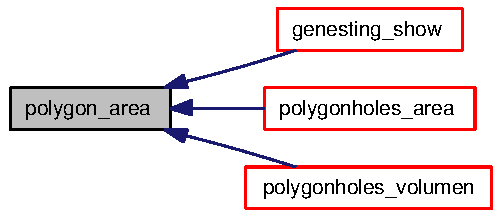
\includegraphics[width=138pt]{group__geometry_gcfbc9e7772d80361768bc0b65cebbca1_gcfbc9e7772d80361768bc0b65cebbca1_icgraph}
\end{center}
\end{figure}
\hypertarget{group__geometry_ge39fef354e4411678ec081c197b29825_ge39fef354e4411678ec081c197b29825}{
\index{geometry@{geometry}!polygon_center@{polygon\_\-center}}
\index{polygon_center@{polygon\_\-center}!geometry@{geometry}}
\subsubsection[polygon\_\-center]{\setlength{\rightskip}{0pt plus 5cm}\hyperlink{struct__point}{point} polygon\_\-center (\hyperlink{struct__polygon}{polygon} $\ast$ {\em p})}}
\label{group__geometry_ge39fef354e4411678ec081c197b29825_ge39fef354e4411678ec081c197b29825}




Definici\'{o}n en la l\'{\i}nea 137 del archivo polygon.c.

\begin{Code}\begin{verbatim}138 {
139     int i=0;
140     float minx, maxx, miny, maxy;
141 
142     point r;
143 
144     polygon_minbox(p, &minx, &miny, &maxx, &maxy)
145 
146     r.x = ((maxx - minx)/2)+minx;
147     r.y = ((maxy - miny)/2)+miny;
148 
149     return r;
150 }
\end{verbatim}\end{Code}




Gr\'{a}fico de llamadas para esta funci\'{o}n:\begin{figure}[H]
\begin{center}
\leavevmode
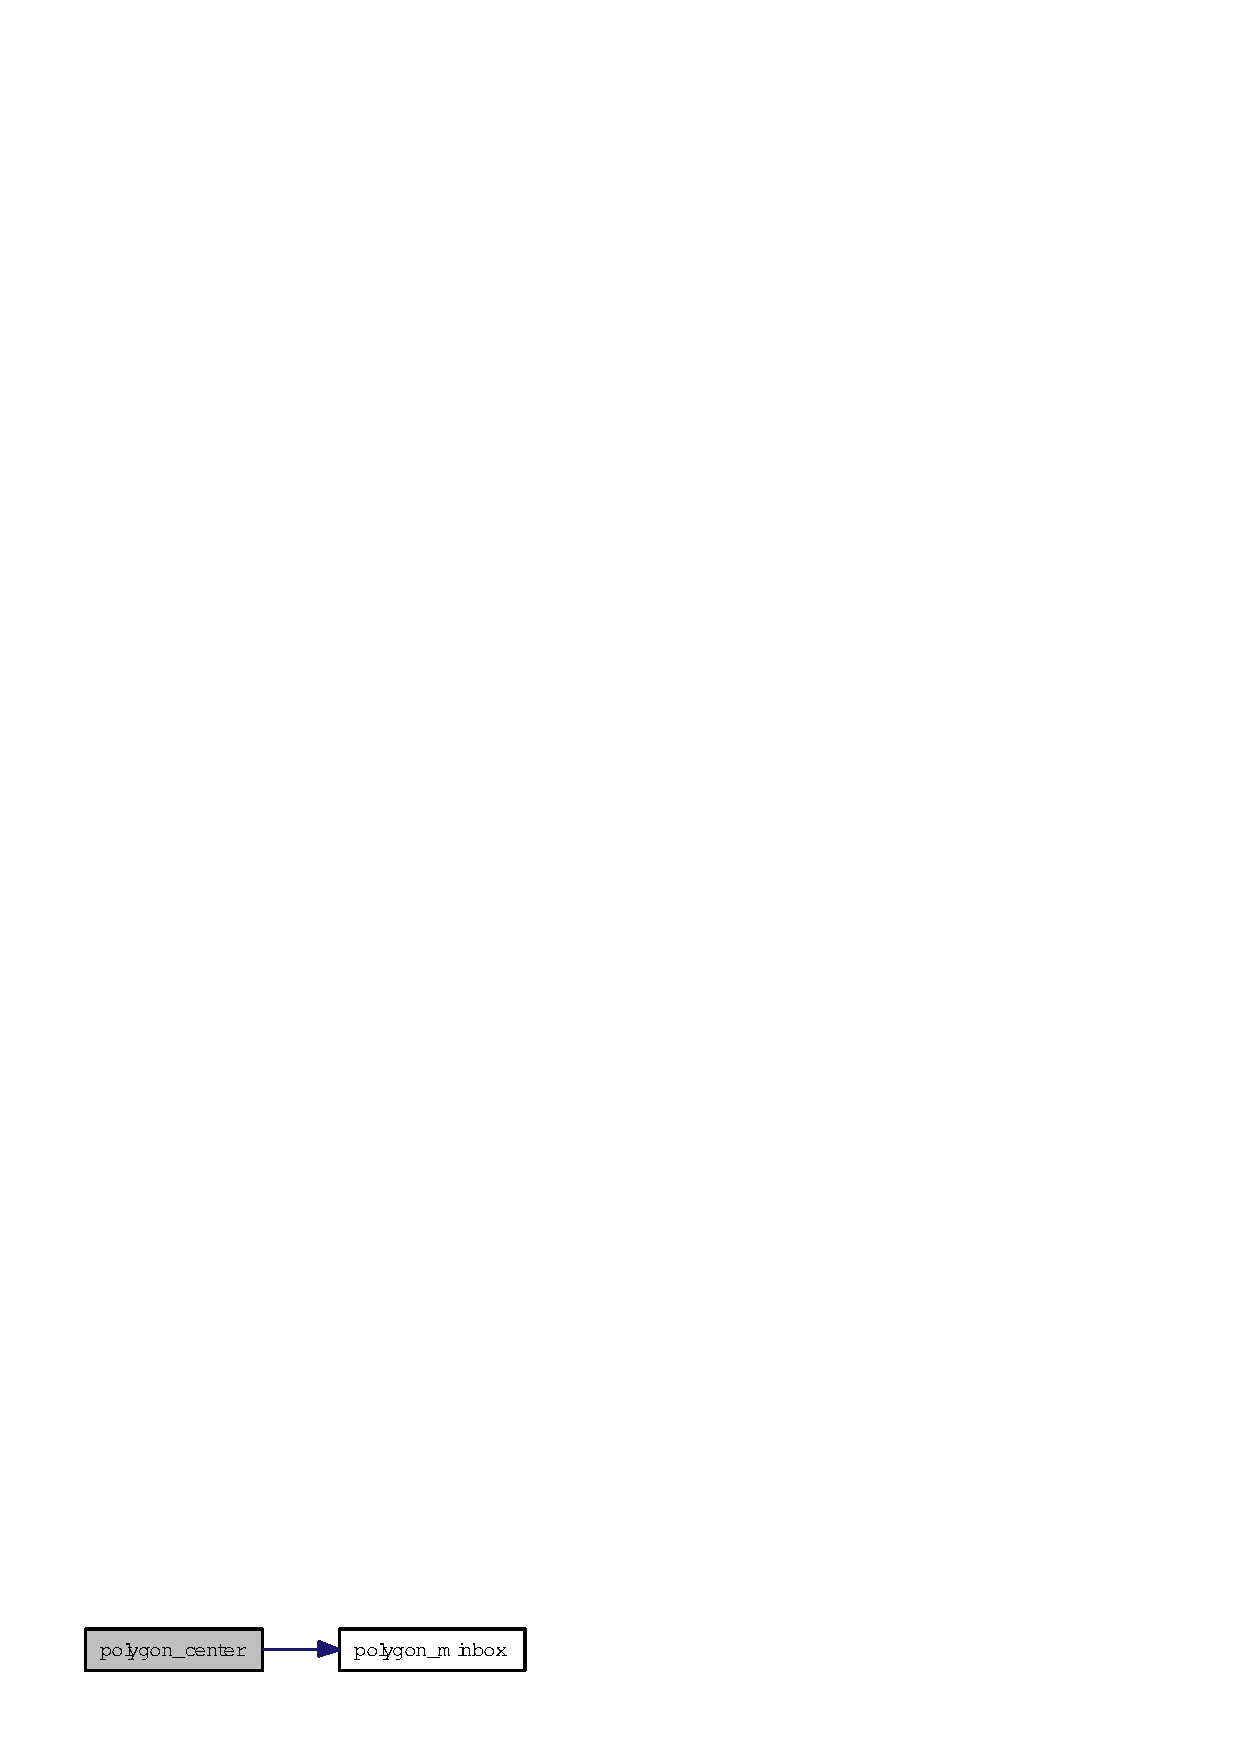
\includegraphics[width=128pt]{group__geometry_ge39fef354e4411678ec081c197b29825_ge39fef354e4411678ec081c197b29825_cgraph}
\end{center}
\end{figure}


Here is the caller graph for this function:\begin{figure}[H]
\begin{center}
\leavevmode
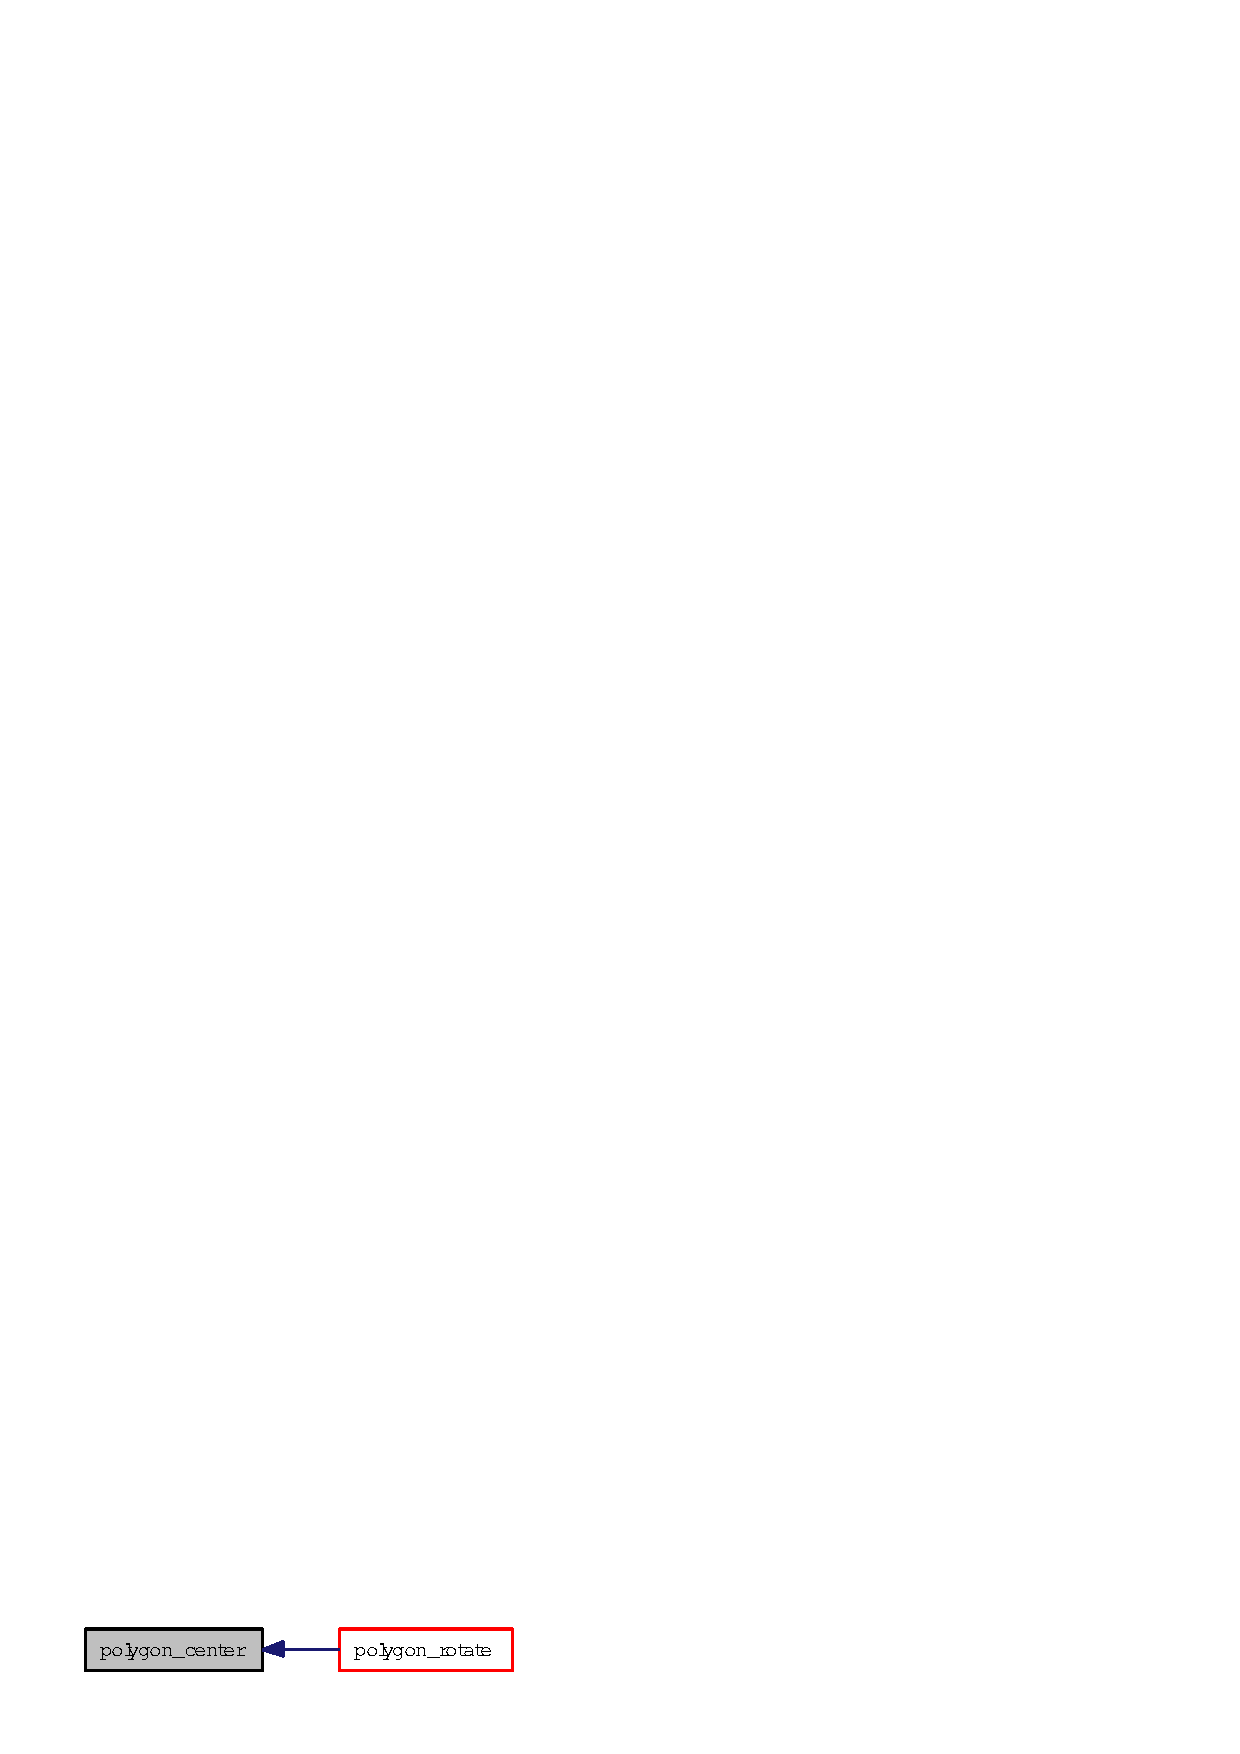
\includegraphics[width=125pt]{group__geometry_ge39fef354e4411678ec081c197b29825_ge39fef354e4411678ec081c197b29825_icgraph}
\end{center}
\end{figure}
\hypertarget{group__geometry_g137ef6f552a0a04c5ae0493690088f3f_g137ef6f552a0a04c5ae0493690088f3f}{
\index{geometry@{geometry}!polygon_minbox@{polygon\_\-minbox}}
\index{polygon_minbox@{polygon\_\-minbox}!geometry@{geometry}}
\subsubsection[polygon\_\-minbox]{\setlength{\rightskip}{0pt plus 5cm}void polygon\_\-minbox (\hyperlink{struct__polygon}{polygon} $\ast$ {\em p}, float $\ast$ {\em minx}, float $\ast$ {\em miny}, float $\ast$ {\em maxx}, float $\ast$ {\em maxy})}}
\label{group__geometry_g137ef6f552a0a04c5ae0493690088f3f_g137ef6f552a0a04c5ae0493690088f3f}


La funcion calcula las coordenadas mas extremas del poligono, conformando con estas 2 puntos que pueden formar un rectangulo que contiene completamente el poligono

\begin{Desc}
\item[Par\'{a}metros:]
\begin{description}
\item[\mbox{$\leftarrow$} {\em p}]Poligono simple \item[\mbox{$\rightarrow$} {\em minx}]Coordenada mas peque\~{n}a del poligono en el eje x \item[\mbox{$\rightarrow$} {\em miny}]Coordenada mas peque\~{n}a del poligono en el eje y \item[\mbox{$\rightarrow$} {\em maxx}]Coordenada mas grande del poligono en el eje x \item[\mbox{$\rightarrow$} {\em maxy}]Coordenada mas grande del poligono en el eje y \end{description}
\end{Desc}


Definici\'{o}n en la l\'{\i}nea 163 del archivo polygon.c.

\begin{Code}\begin{verbatim}164 {
165     int i;
166 
167     *minx = p->v[0].x;
168     *miny = p->v[0].y;
169     *maxx = p->v[0].x;
170     *maxy = p->v[0].y;
171 
172     for (i=1;i<p->nvertices;i++)
173     {
174         if (*minx > p->v[i].x)
175         {
176             *minx = p->v[i].x;
177         }
178         if (*miny > p->v[i].y)
179         {
180             *miny = p->v[i].y;
181         }
182         if (*maxx < p->v[i].x)
183         {
184             *maxx = p->v[i].x;
185         }
186         if (*maxy < p->v[i].y)
187         {
188             *maxy = p->v[i].y;
189         }
190     }
191 }
\end{verbatim}\end{Code}




Here is the caller graph for this function:\begin{figure}[H]
\begin{center}
\leavevmode
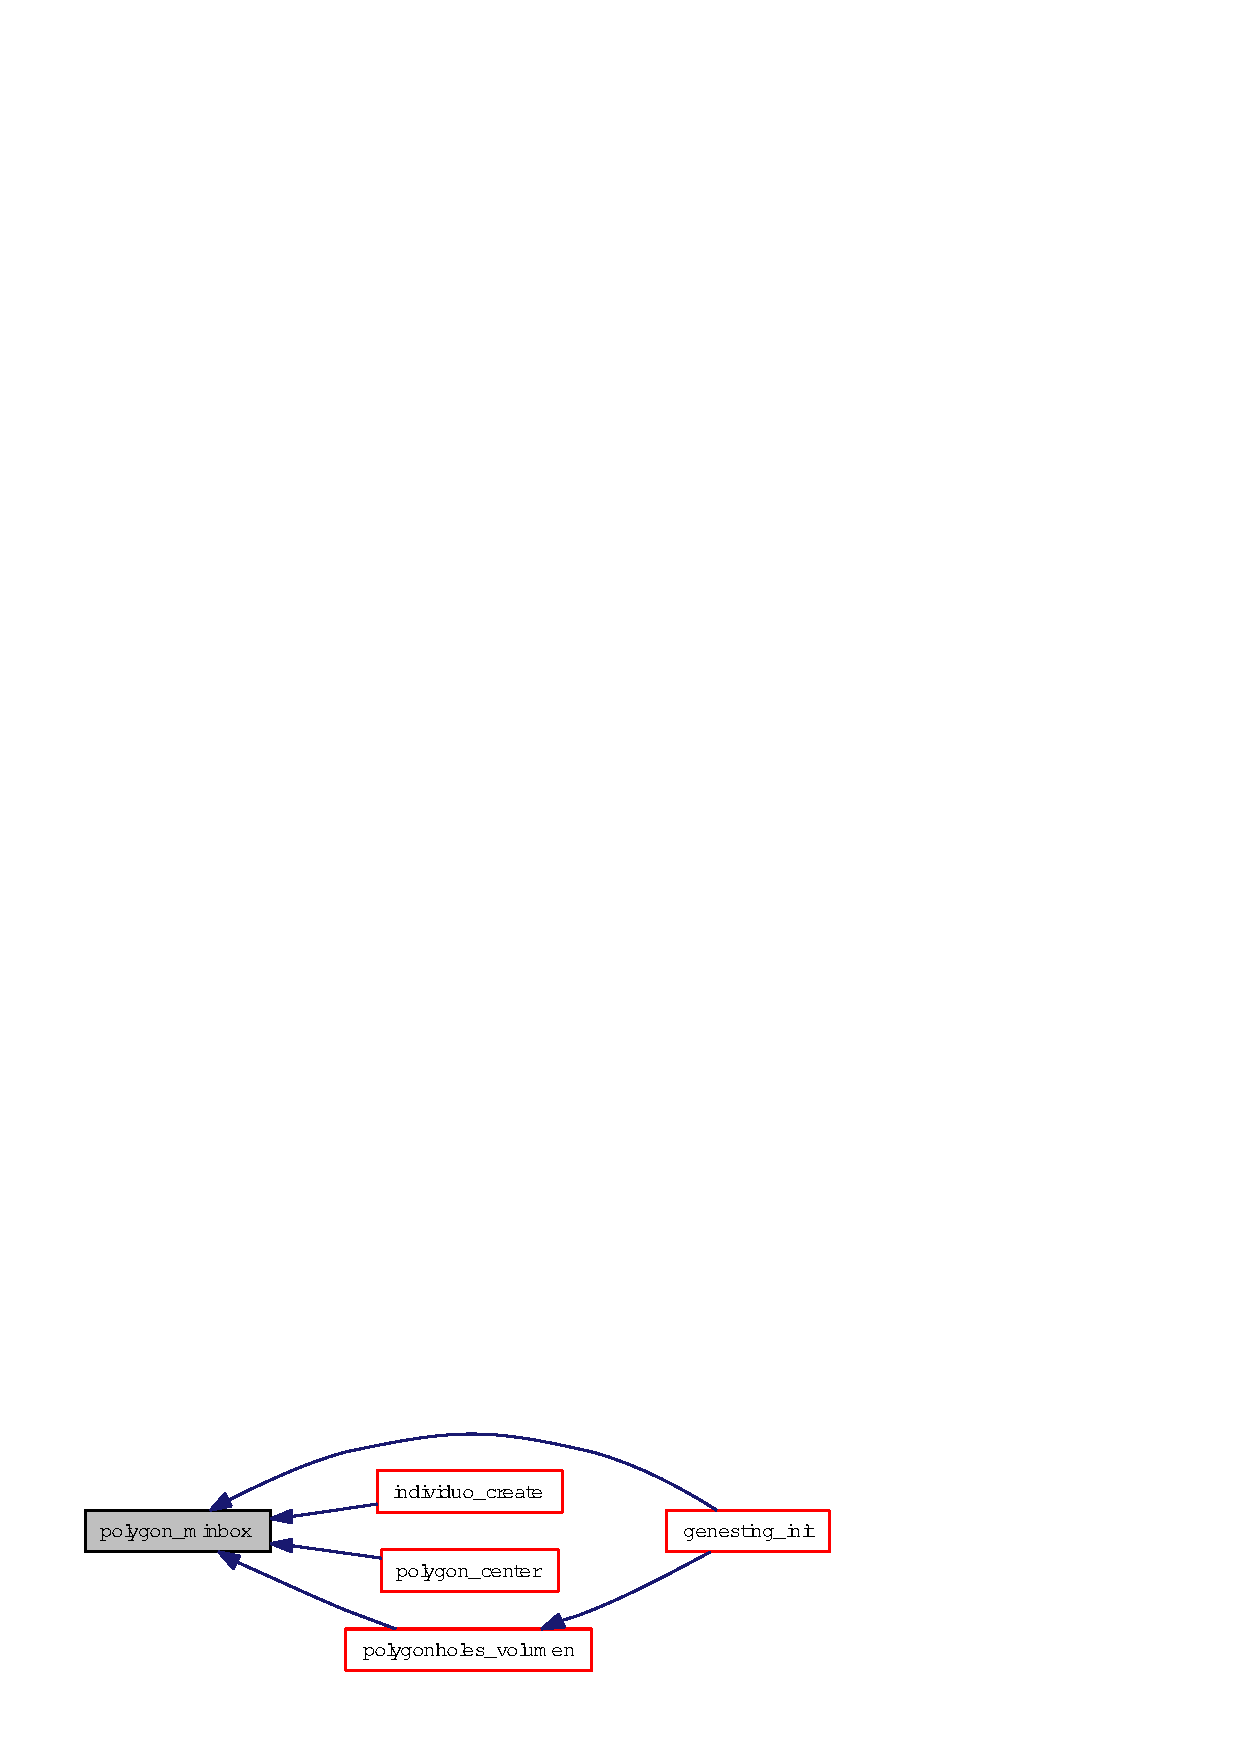
\includegraphics[width=201pt]{group__geometry_g137ef6f552a0a04c5ae0493690088f3f_g137ef6f552a0a04c5ae0493690088f3f_icgraph}
\end{center}
\end{figure}
\hypertarget{group__geometry_g2be6101a257ea8896e61e93d14b22b89_g2be6101a257ea8896e61e93d14b22b89}{
\index{geometry@{geometry}!polygon_overlapping@{polygon\_\-overlapping}}
\index{polygon_overlapping@{polygon\_\-overlapping}!geometry@{geometry}}
\subsubsection[polygon\_\-overlapping]{\setlength{\rightskip}{0pt plus 5cm}bool polygon\_\-overlapping (\hyperlink{struct__polygon}{polygon} $\ast$ {\em p}, \hyperlink{struct__polygon}{polygon} $\ast$ {\em q})}}
\label{group__geometry_g2be6101a257ea8896e61e93d14b22b89_g2be6101a257ea8896e61e93d14b22b89}


Esta funcion identifica si dos poligonos se solapan de alguna forma para verificar esto se realizan 3 comprobaciones:\begin{itemize}
\item Ningun vertice del poligono p esta dentro del poligono q\item Ningun vertice del poligono q esta dentro del poligono p\item Ninguna linea de los poligonos p y q se intersectan\end{itemize}


\begin{Desc}
\item[Par\'{a}metros:]
\begin{description}
\item[\mbox{$\leftarrow$} {\em p}]Poligono Simple en 2 dimensiones \item[\mbox{$\leftarrow$} {\em q}]Poligono Simple en 2 dimensiones \end{description}
\end{Desc}
\begin{Desc}
\item[Devuelve:]Verdadero si los poligonos se solapan, falso en caso contrario. \end{Desc}


Definici\'{o}n en la l\'{\i}nea 74 del archivo polygon.c.

\begin{Code}\begin{verbatim}75 {
76     int i,j;
77 
78     for (i=0;i<p->nvertices;i++)
79     {
80         if (polygon_pointin(q,&p->v[i]))
81             return true;
82     }
83 
84     for (i=0;i<q->nvertices;i++)
85     {
86         if (polygon_pointin(p,&q->v[i]))
87             return true;
88     }
89 
90     for (i=0;i<p->nvertices;i++)
91     {
92         line t1,t2;
93         t1.v1=p->v[i];
94         t1.v2=p->v[(i+1)%(p->nvertices)];
95         for (j=0;j<q->nvertices;j++)
96         {
97             t2.v1=q->v[j];
98             t2.v2=q->v[(j+1)%q->nvertices];
99             if (line_intersection(&t1,&t2))
100                 return true;
101         }
102     }
103     return false;
104 }
\end{verbatim}\end{Code}




Gr\'{a}fico de llamadas para esta funci\'{o}n:\begin{figure}[H]
\begin{center}
\leavevmode
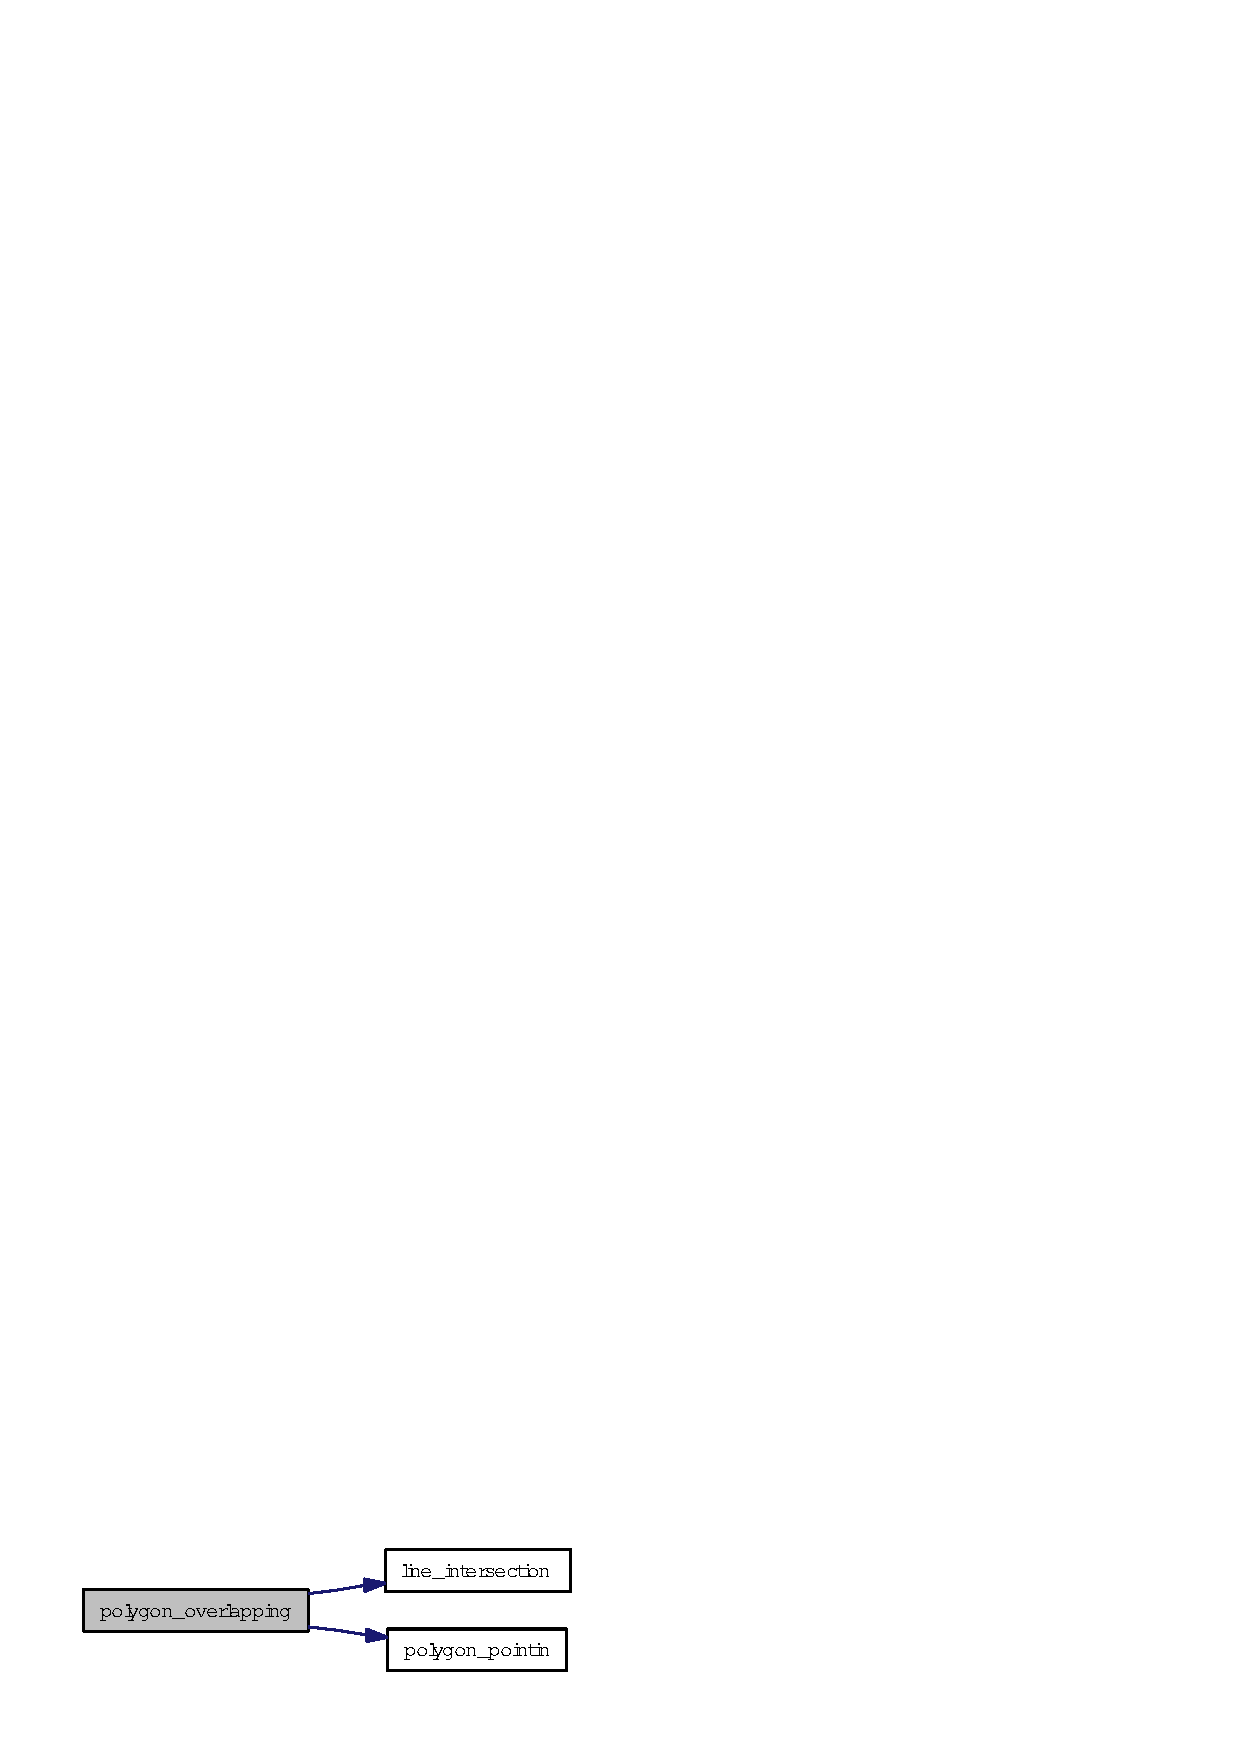
\includegraphics[width=139pt]{group__geometry_g2be6101a257ea8896e61e93d14b22b89_g2be6101a257ea8896e61e93d14b22b89_cgraph}
\end{center}
\end{figure}


Here is the caller graph for this function:\begin{figure}[H]
\begin{center}
\leavevmode
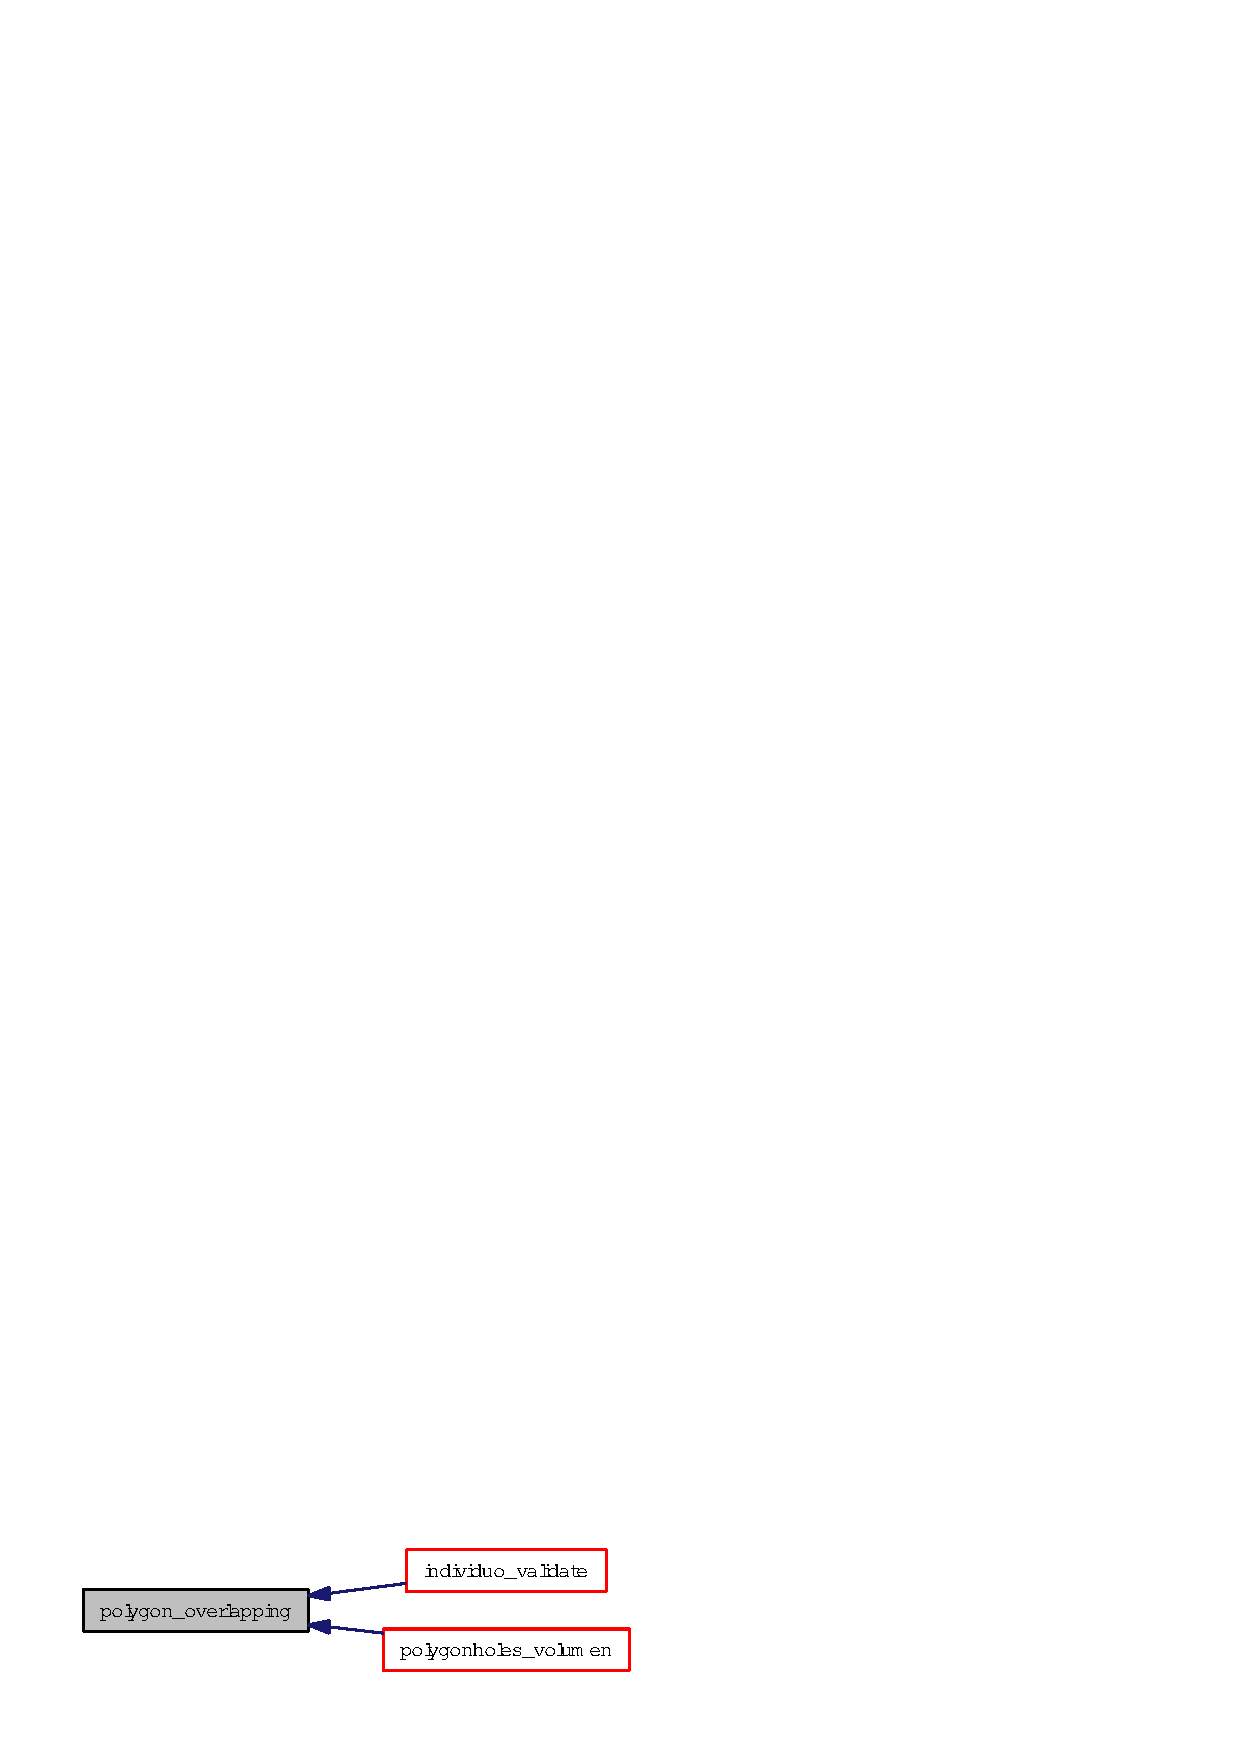
\includegraphics[width=153pt]{group__geometry_g2be6101a257ea8896e61e93d14b22b89_g2be6101a257ea8896e61e93d14b22b89_icgraph}
\end{center}
\end{figure}
\hypertarget{group__geometry_geab0a1d6da7c44ae49494958bb885504_geab0a1d6da7c44ae49494958bb885504}{
\index{geometry@{geometry}!polygon_pointin@{polygon\_\-pointin}}
\index{polygon_pointin@{polygon\_\-pointin}!geometry@{geometry}}
\subsubsection[polygon\_\-pointin]{\setlength{\rightskip}{0pt plus 5cm}bool polygon\_\-pointin (\hyperlink{struct__polygon}{polygon} $\ast$ {\em p}, \hyperlink{struct__point}{point} $\ast$ {\em f})}}
\label{group__geometry_geab0a1d6da7c44ae49494958bb885504_geab0a1d6da7c44ae49494958bb885504}


La funcion identifica si un punto esta dentro de un poligono o no.

\begin{Desc}
\item[Par\'{a}metros:]
\begin{description}
\item[\mbox{$\leftarrow$} {\em p}]Poligono simple en 2 dimensiones \item[\mbox{$\leftarrow$} {\em f}]Punto en 2 dimensiones \end{description}
\end{Desc}
\begin{Desc}
\item[Devuelve:]Un booleano que es verdadero en caso de que el punto este dentro del poligono y falso en caso contrario \end{Desc}


Definici\'{o}n en la l\'{\i}nea 48 del archivo polygon.c.

\begin{Code}\begin{verbatim}49 {
50     bool c=false;
51     unsigned int i,j;
52 
53     for (i=0,j=p->nvertices-1;i<p->nvertices;j=i++)
54     {
55         if ((((p->v[i].y<=f->y) && (f->y<p->v[j].y)) ||
56                 ((p->v[j].y<=f->y) && (f->y<p->v[i].y))) &&
57                 (f->x < (p->v[j].x - p->v[i].x) * (f->y - p->v[i].y) / (p->v[j].y - p->v[i].y) + p->v[i].x))
58             c = !c;
59     }
60     return c;
61 }
\end{verbatim}\end{Code}




Here is the caller graph for this function:\begin{figure}[H]
\begin{center}
\leavevmode
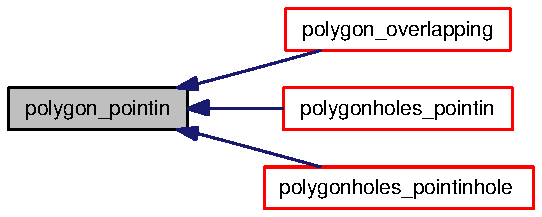
\includegraphics[width=148pt]{group__geometry_geab0a1d6da7c44ae49494958bb885504_geab0a1d6da7c44ae49494958bb885504_icgraph}
\end{center}
\end{figure}
\hypertarget{group__geometry_g95276abee7240f116afaf80a3e1f23c4_g95276abee7240f116afaf80a3e1f23c4}{
\index{geometry@{geometry}!polygon_rotate@{polygon\_\-rotate}}
\index{polygon_rotate@{polygon\_\-rotate}!geometry@{geometry}}
\subsubsection[polygon\_\-rotate]{\setlength{\rightskip}{0pt plus 5cm}void polygon\_\-rotate (\hyperlink{struct__polygon}{polygon} $\ast$ {\em p}, float {\em t})}}
\label{group__geometry_g95276abee7240f116afaf80a3e1f23c4_g95276abee7240f116afaf80a3e1f23c4}


La funcion rota el poligono p un angulo t, teniendo como eje de rotacion el centro de la caja mas pequena que contiene el poligono. Aunque se pueden elegir otros puntos como eje, o de hecho implementar un eje arbitrario, el centro de la caja que contiene el poligono es un punto facil de calcular y ademas que evita exageradas translaciones relativas del poligono al ser rotado.

\begin{Desc}
\item[Par\'{a}metros:]
\begin{description}
\item[\mbox{$\leftrightarrow$} {\em p}]Poligono simple \item[\mbox{$\leftarrow$} {\em t}]Angulo en radianes a rotar la figura en sentido antihorario. \end{description}
\end{Desc}


Definici\'{o}n en la l\'{\i}nea 116 del archivo polygon.c.

\begin{Code}\begin{verbatim}117 {
118     int i;
119     point pc;
120 
121     float sent = sin(t);
122     float cost = cos(t);
123 
124     pc = polygon_center(p);
125 
126     polygon_translate(p, -pc.x, -pc.y);
127 
128     for (i=0;i<p->nvertices;i++)
129     {
130         p->v[i].x=(p->v[i].x*cost - p->v[i].y * sent);
131         p->v[i].y=(p->v[i].y*cost + p->v[i].x * sent);
132     }
133 
134     polygon_translate(p, pc.x, pc.y);
135 }
\end{verbatim}\end{Code}




Gr\'{a}fico de llamadas para esta funci\'{o}n:\begin{figure}[H]
\begin{center}
\leavevmode
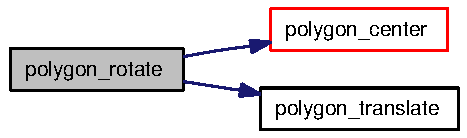
\includegraphics[width=130pt]{group__geometry_g95276abee7240f116afaf80a3e1f23c4_g95276abee7240f116afaf80a3e1f23c4_cgraph}
\end{center}
\end{figure}


Here is the caller graph for this function:\begin{figure}[H]
\begin{center}
\leavevmode
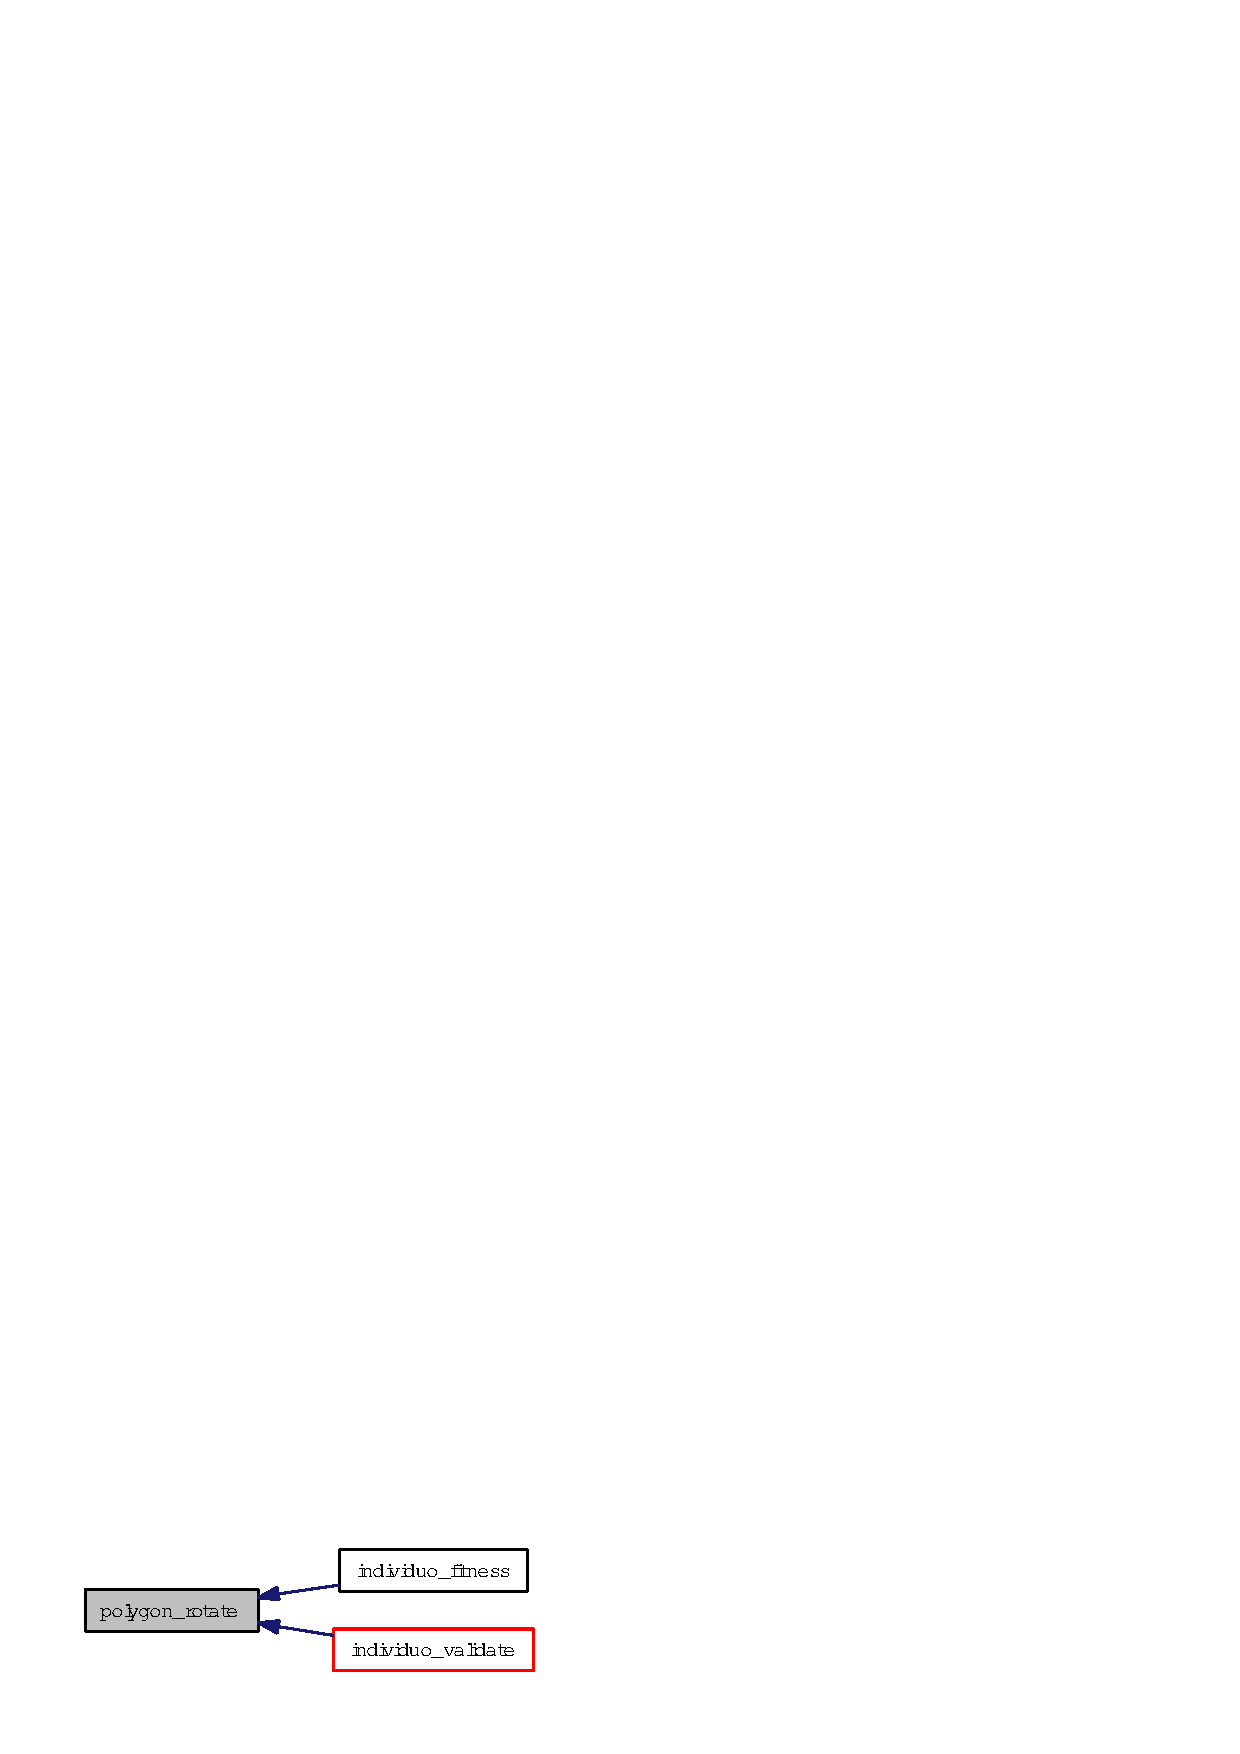
\includegraphics[width=130pt]{group__geometry_g95276abee7240f116afaf80a3e1f23c4_g95276abee7240f116afaf80a3e1f23c4_icgraph}
\end{center}
\end{figure}
\hypertarget{group__geometry_g7538c2bf0d1e8acc0cfc055b6bf3a96b_g7538c2bf0d1e8acc0cfc055b6bf3a96b}{
\index{geometry@{geometry}!polygon_translate@{polygon\_\-translate}}
\index{polygon_translate@{polygon\_\-translate}!geometry@{geometry}}
\subsubsection[polygon\_\-translate]{\setlength{\rightskip}{0pt plus 5cm}void polygon\_\-translate (\hyperlink{struct__polygon}{polygon} $\ast$ {\em p}, float {\em x}, float {\em y})}}
\label{group__geometry_g7538c2bf0d1e8acc0cfc055b6bf3a96b_g7538c2bf0d1e8acc0cfc055b6bf3a96b}


Translada el poligono una distancia definida por x,y.

\begin{Desc}
\item[Par\'{a}metros:]
\begin{description}
\item[\mbox{$\leftrightarrow$} {\em p}]Poligono simple \item[\mbox{$\leftarrow$} {\em x}]Distancia en x a transladar el poligono \item[\mbox{$\leftarrow$} {\em y}]Distancia en y a transladar el poligono \end{description}
\end{Desc}


Definici\'{o}n en la l\'{\i}nea 200 del archivo polygon.c.

\begin{Code}\begin{verbatim}201 {
202     int i;
203     for (i=0;i<p->nvertices;i++)
204     {
205         p->v[i].x+=x;
206         p->v[i].y+=y;
207     }
208 }
\end{verbatim}\end{Code}




Here is the caller graph for this function:\begin{figure}[H]
\begin{center}
\leavevmode
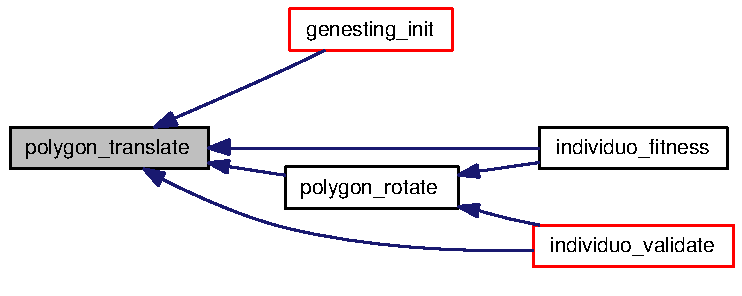
\includegraphics[width=196pt]{group__geometry_g7538c2bf0d1e8acc0cfc055b6bf3a96b_g7538c2bf0d1e8acc0cfc055b6bf3a96b_icgraph}
\end{center}
\end{figure}
\hypertarget{group__geometry_g380cdcfa6caf51828c8d06f4518a4084_g380cdcfa6caf51828c8d06f4518a4084}{
\index{geometry@{geometry}!polygonholes_area@{polygonholes\_\-area}}
\index{polygonholes_area@{polygonholes\_\-area}!geometry@{geometry}}
\subsubsection[polygonholes\_\-area]{\setlength{\rightskip}{0pt plus 5cm}float polygonholes\_\-area (\hyperlink{struct__polygon__holes}{polygon\_\-holes} $\ast$ {\em p})}}
\label{group__geometry_g380cdcfa6caf51828c8d06f4518a4084_g380cdcfa6caf51828c8d06f4518a4084}


La funcion calcula el area de un Poligono con huecos, para hacer esto calculamos el area del poligono formado por el borde exterior y le restamos el area de cada uno de los huecos.

\begin{Desc}
\item[Par\'{a}metros:]
\begin{description}
\item[\mbox{$\leftarrow$} {\em p}]Poligono simple en 2 dimensiones \end{description}
\end{Desc}
\begin{Desc}
\item[Devuelve:]Area del poligono simple con huecos \end{Desc}


Definici\'{o}n en la l\'{\i}nea 30 del archivo polygon\_\-holes.c.

\begin{Code}\begin{verbatim}31 {
32     unsigned int i;
33     float area;
34     area = polygon_area(p->p);
35     for (i=0;i<p->nholes;i++)
36     {
37         area -= polygon_area(&(p->h[i]));
38     }
39     return area;
40 }
\end{verbatim}\end{Code}




Gr\'{a}fico de llamadas para esta funci\'{o}n:\begin{figure}[H]
\begin{center}
\leavevmode
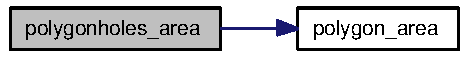
\includegraphics[width=130pt]{group__geometry_g380cdcfa6caf51828c8d06f4518a4084_g380cdcfa6caf51828c8d06f4518a4084_cgraph}
\end{center}
\end{figure}


Here is the caller graph for this function:\begin{figure}[H]
\begin{center}
\leavevmode
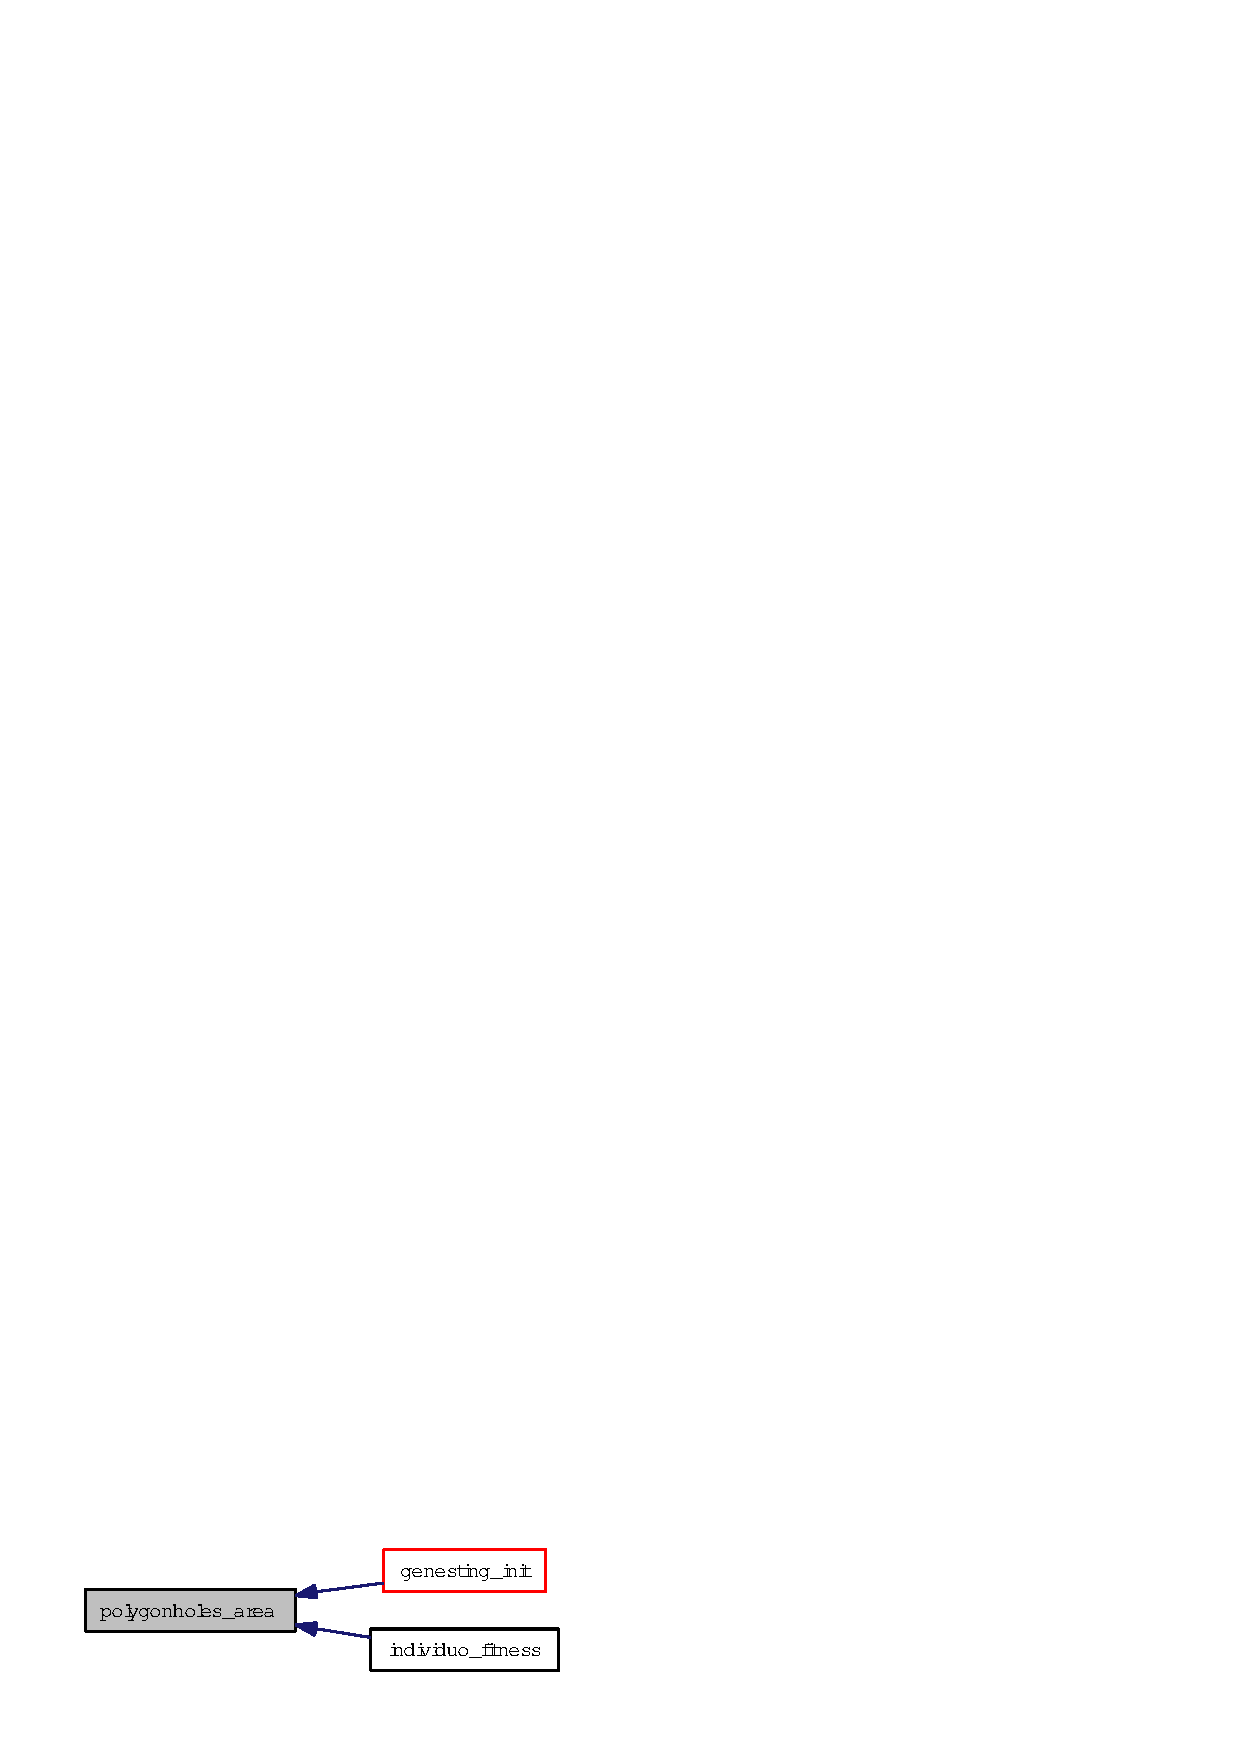
\includegraphics[width=136pt]{group__geometry_g380cdcfa6caf51828c8d06f4518a4084_g380cdcfa6caf51828c8d06f4518a4084_icgraph}
\end{center}
\end{figure}
\hypertarget{group__geometry_g35a6dd45f6d0cbed26ef8a69ed34a2e9_g35a6dd45f6d0cbed26ef8a69ed34a2e9}{
\index{geometry@{geometry}!polygonholes_pointin@{polygonholes\_\-pointin}}
\index{polygonholes_pointin@{polygonholes\_\-pointin}!geometry@{geometry}}
\subsubsection[polygonholes\_\-pointin]{\setlength{\rightskip}{0pt plus 5cm}bool polygonholes\_\-pointin (\hyperlink{struct__polygon__holes}{polygon\_\-holes} $\ast$ {\em p}, \hyperlink{struct__point}{point} $\ast$ {\em f})}}
\label{group__geometry_g35a6dd45f6d0cbed26ef8a69ed34a2e9_g35a6dd45f6d0cbed26ef8a69ed34a2e9}


Esta funcion identifica si un punto esta dentro de un poligono con huecos por lo tanto evalua inicialmente que el punto este dentro del poligono exterior y posterioremente que no se encuentre dentro de los huecos

\begin{Desc}
\item[Par\'{a}metros:]
\begin{description}
\item[\mbox{$\leftarrow$} {\em p}]Poligono simple con huecos en 2 dimensiones \item[\mbox{$\leftarrow$} {\em f}]Punto en 2 dimensiones \end{description}
\end{Desc}
\begin{Desc}
\item[Devuelve:]Verdadero en caso que el punto este dentro del poligono, falso en caso contrario \end{Desc}


Definici\'{o}n en la l\'{\i}nea 345 del archivo polygon\_\-holes.c.

\begin{Code}\begin{verbatim}346 {
347     bool valido=false;
348     if (polygon_pointin(p->p, f))
349     {
350         unsigned int i;
351         valido=true;
352 
353         for (i=0;i<p->nholes && valido;i++)
354         {
355             if (polygon_pointin(&(p->h[i]), f))
356             {
357                 valido=false;
358             }
359         }
360     }
361     return valido;
362 }
\end{verbatim}\end{Code}




Gr\'{a}fico de llamadas para esta funci\'{o}n:\begin{figure}[H]
\begin{center}
\leavevmode
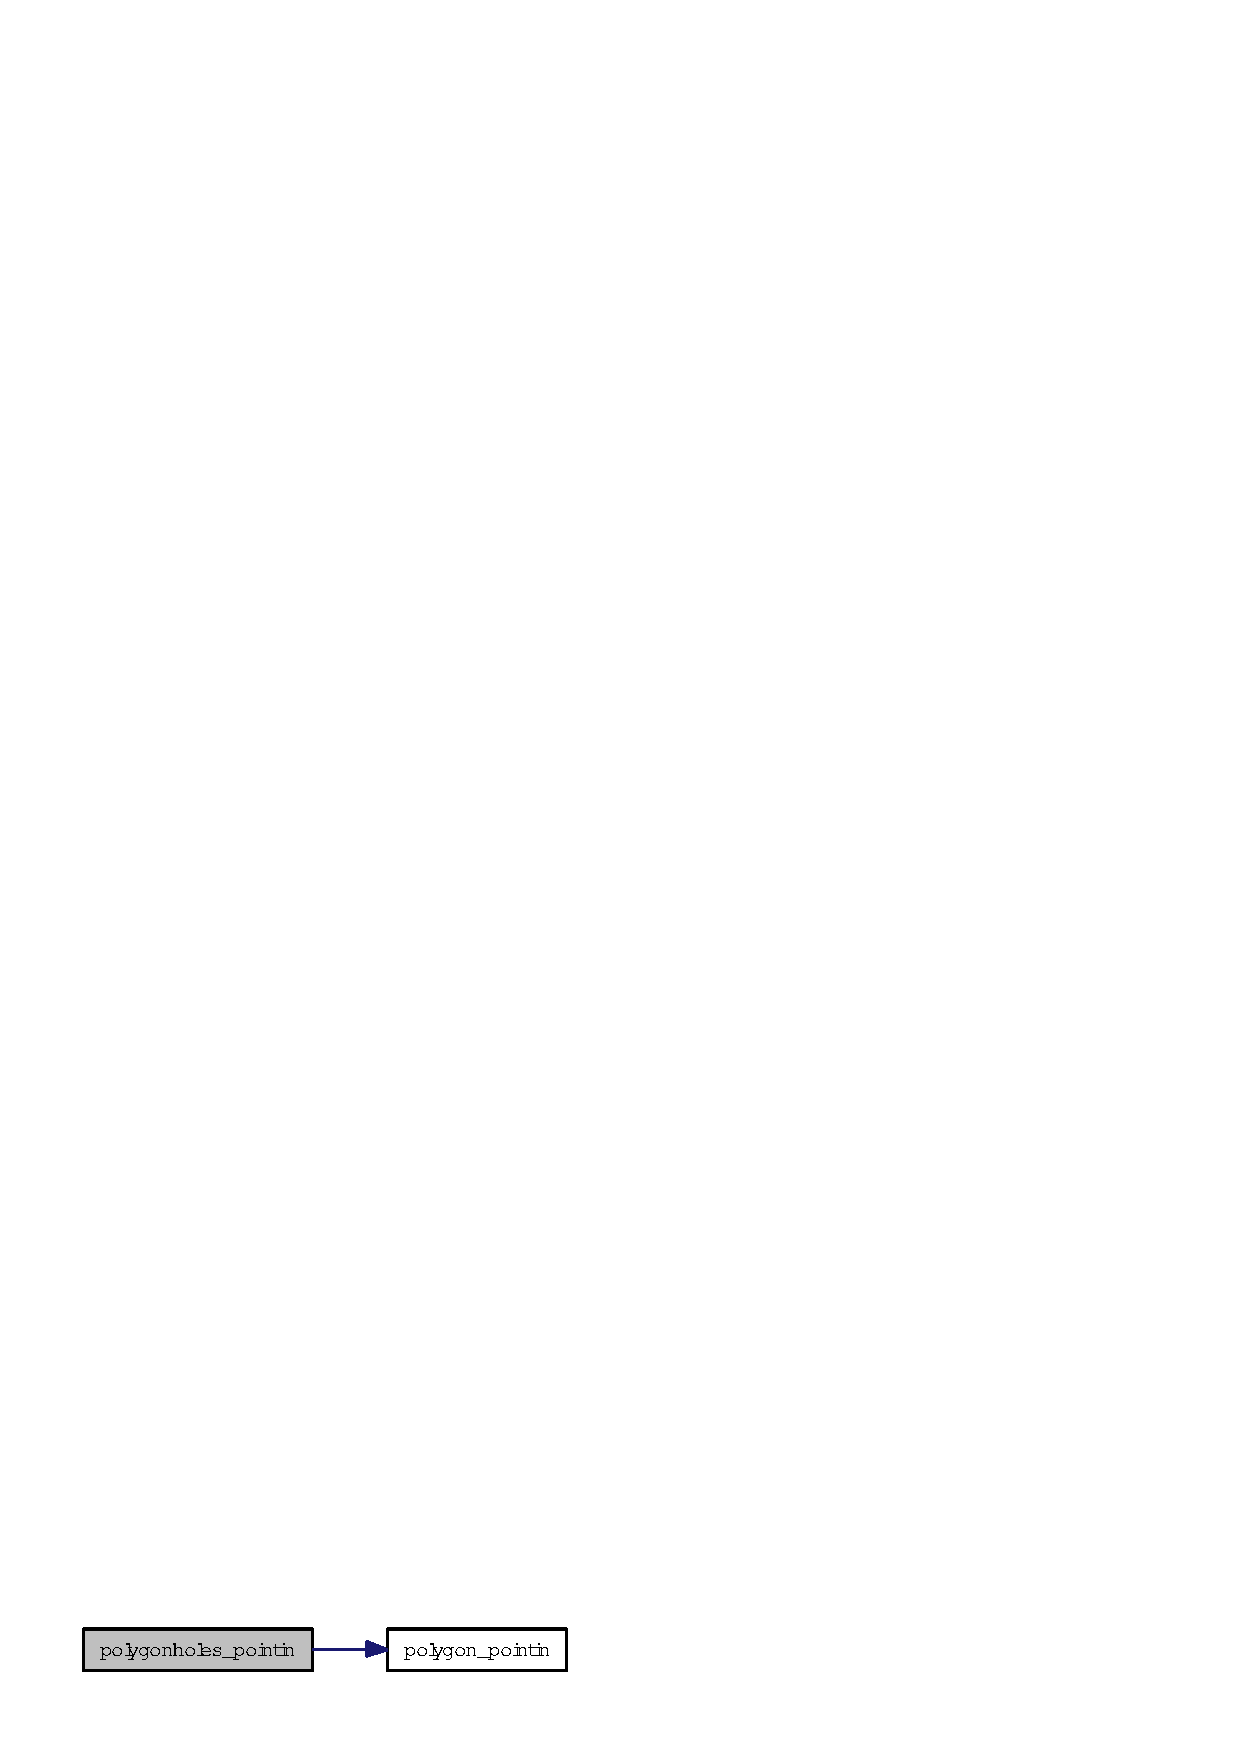
\includegraphics[width=138pt]{group__geometry_g35a6dd45f6d0cbed26ef8a69ed34a2e9_g35a6dd45f6d0cbed26ef8a69ed34a2e9_cgraph}
\end{center}
\end{figure}


Here is the caller graph for this function:\begin{figure}[H]
\begin{center}
\leavevmode
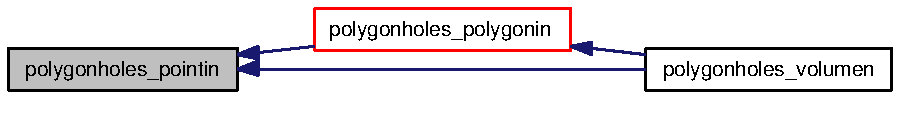
\includegraphics[width=234pt]{group__geometry_g35a6dd45f6d0cbed26ef8a69ed34a2e9_g35a6dd45f6d0cbed26ef8a69ed34a2e9_icgraph}
\end{center}
\end{figure}
\hypertarget{group__geometry_g139317720b027c782db9424256ba2c2d_g139317720b027c782db9424256ba2c2d}{
\index{geometry@{geometry}!polygonholes_pointinhole@{polygonholes\_\-pointinhole}}
\index{polygonholes_pointinhole@{polygonholes\_\-pointinhole}!geometry@{geometry}}
\subsubsection[polygonholes\_\-pointinhole]{\setlength{\rightskip}{0pt plus 5cm}bool polygonholes\_\-pointinhole (\hyperlink{struct__polygon__holes}{polygon\_\-holes} $\ast$ {\em p}, \hyperlink{struct__point}{point} $\ast$ {\em f})}}
\label{group__geometry_g139317720b027c782db9424256ba2c2d_g139317720b027c782db9424256ba2c2d}


Identifica si un punto esta dentro de un hueco del poligono.

\begin{Desc}
\item[Par\'{a}metros:]
\begin{description}
\item[\mbox{$\leftarrow$} {\em p}]Poligono Simple con huecos \item[\mbox{$\leftarrow$} {\em f}]Punto en 2 dimensiones \end{description}
\end{Desc}
\begin{Desc}
\item[Devuelve:]Verdadero si el punto esta dentro de uno de los huecos, falso en caso contrario \end{Desc}


Definici\'{o}n en la l\'{\i}nea 373 del archivo polygon\_\-holes.c.

\begin{Code}\begin{verbatim}374 {
375     bool valido=false;
376     unsigned int i;
377 
378     for (i=0;i<p->nholes && !valido;i++)
379     {
380         if (polygon_pointin(&(p->h[i]), f))
381         {
382             valido=true;
383         }
384     }
385     return valido;
386 }
\end{verbatim}\end{Code}




Gr\'{a}fico de llamadas para esta funci\'{o}n:\begin{figure}[H]
\begin{center}
\leavevmode
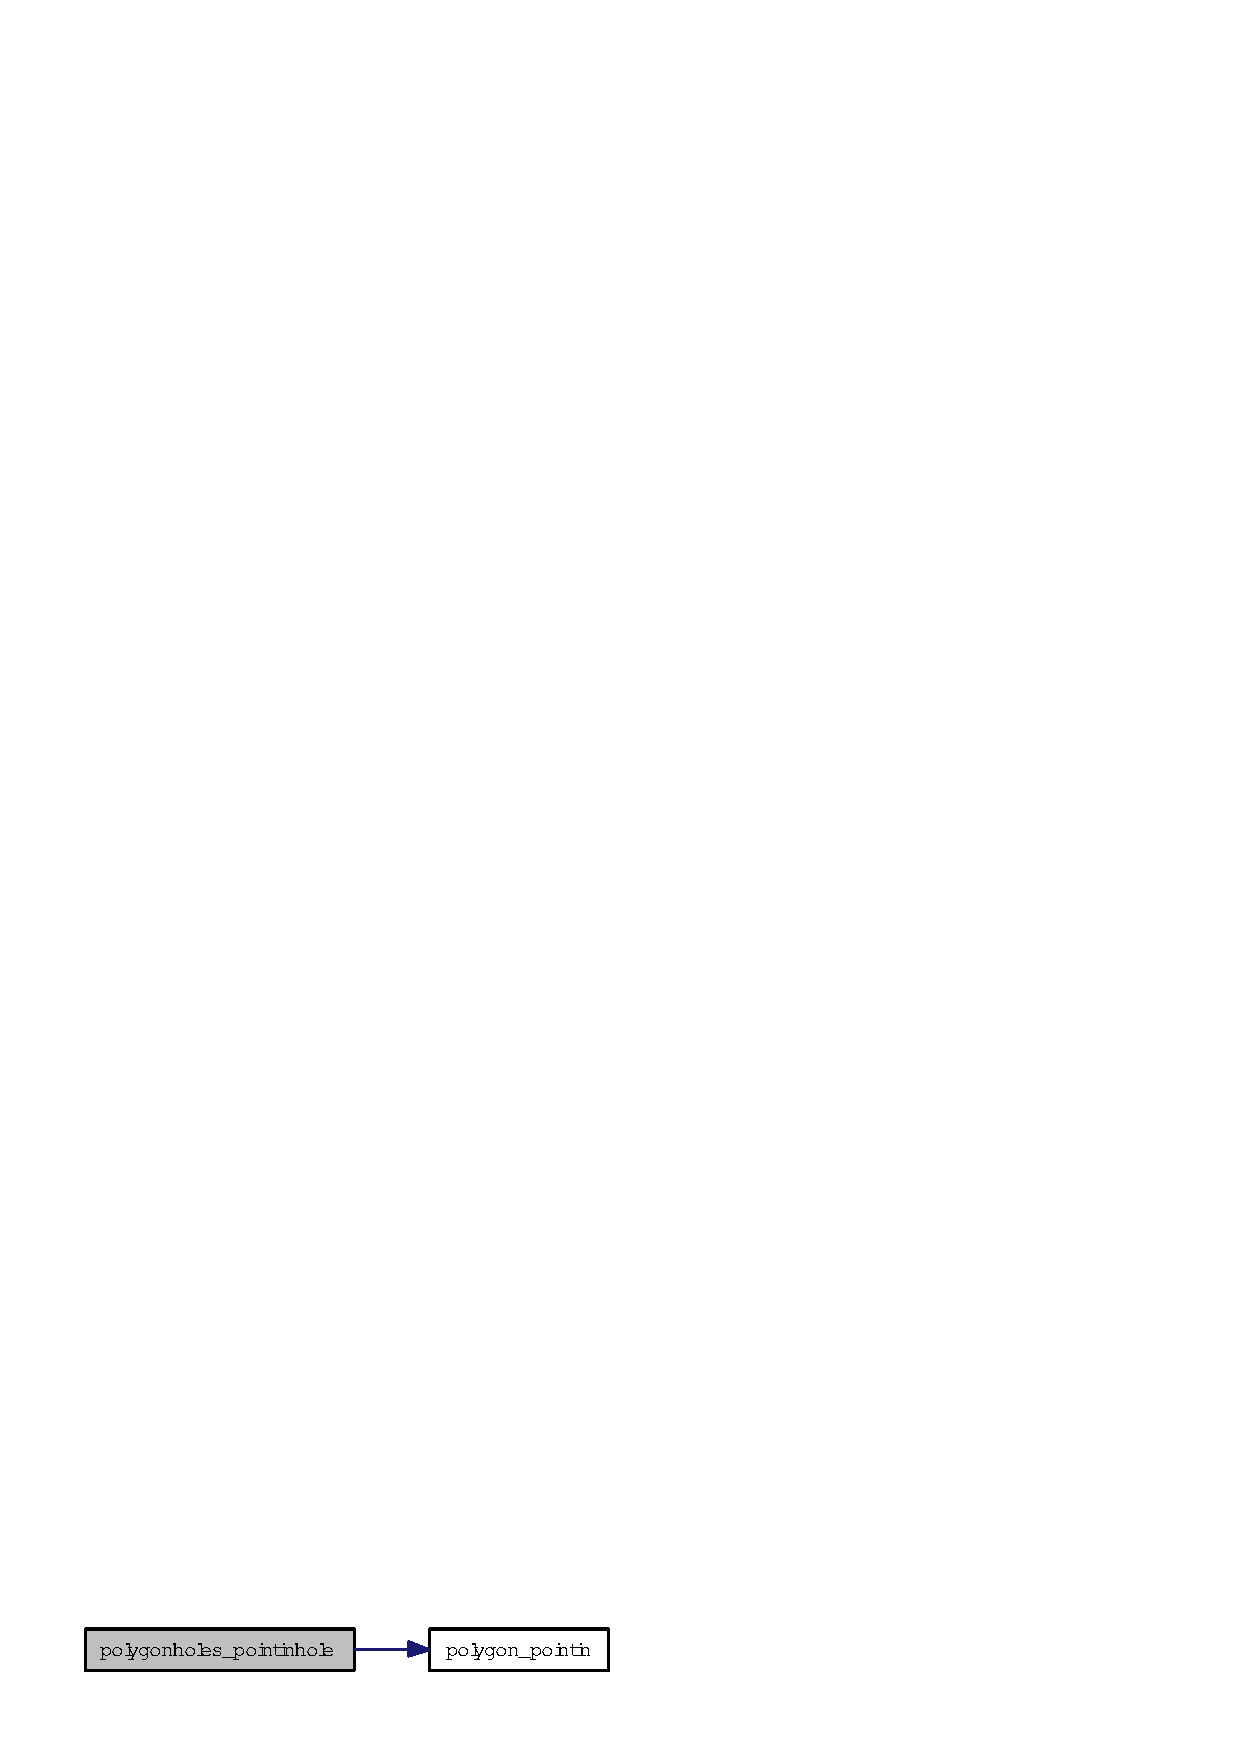
\includegraphics[width=148pt]{group__geometry_g139317720b027c782db9424256ba2c2d_g139317720b027c782db9424256ba2c2d_cgraph}
\end{center}
\end{figure}


Here is the caller graph for this function:\begin{figure}[H]
\begin{center}
\leavevmode
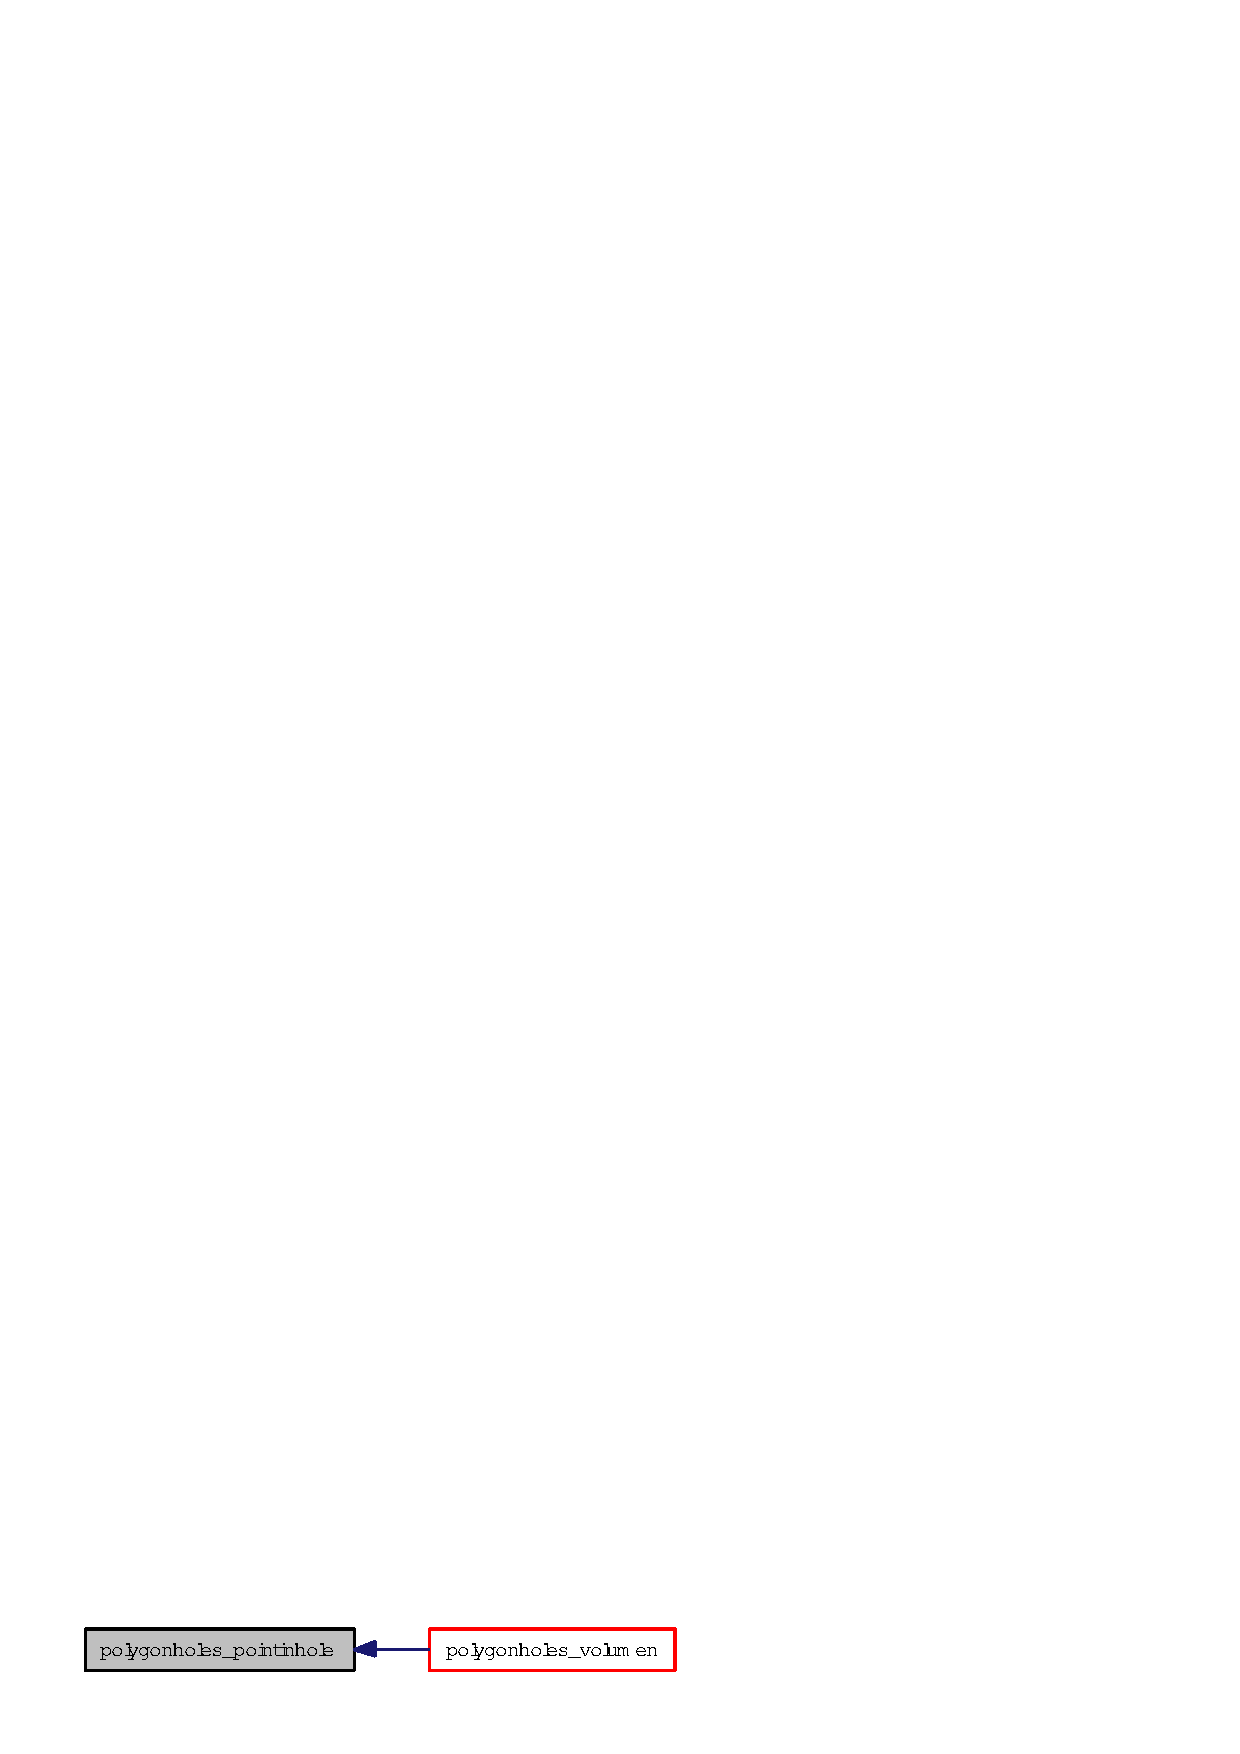
\includegraphics[width=164pt]{group__geometry_g139317720b027c782db9424256ba2c2d_g139317720b027c782db9424256ba2c2d_icgraph}
\end{center}
\end{figure}
\hypertarget{group__geometry_g496bae87588cb5710ced80f713da98ad_g496bae87588cb5710ced80f713da98ad}{
\index{geometry@{geometry}!polygonholes_polygonin@{polygonholes\_\-polygonin}}
\index{polygonholes_polygonin@{polygonholes\_\-polygonin}!geometry@{geometry}}
\subsubsection[polygonholes\_\-polygonin]{\setlength{\rightskip}{0pt plus 5cm}bool polygonholes\_\-polygonin (\hyperlink{struct__polygon__holes}{polygon\_\-holes} $\ast$ {\em p}, \hyperlink{struct__polygon}{polygon} $\ast$ {\em q})}}
\label{group__geometry_g496bae87588cb5710ced80f713da98ad_g496bae87588cb5710ced80f713da98ad}


La funcion evalua que el poligono q esta completamente adentro del poligono p entonces todos los puntos de q deben estar dentro de p y no se deben intersectar las lineas que los conforman

\begin{Desc}
\item[Par\'{a}metros:]
\begin{description}
\item[\mbox{$\leftarrow$} {\em p}]Poligono Simple con huecos \item[\mbox{$\leftarrow$} {\em q}]Poligono Simple \end{description}
\end{Desc}
\begin{Desc}
\item[Devuelve:]Verdadero en caso del que poligono q este dentro del poligono p, falso en caso contrario \end{Desc}


Definici\'{o}n en la l\'{\i}nea 399 del archivo polygon\_\-holes.c.

\begin{Code}\begin{verbatim}400 {
401     int i,j,k;
402     bool adentro = true;
403 
404     for (i=0;i<q->nvertices && adentro;i++)
405     {
406         line t1,t2;
407         t1.v1=q->v[i];
408         t1.v2=q->v[(i+1)%(q->nvertices)];
409 
410         if (!polygonholes_pointin(p,&q->v[i]))
411             adentro = false;
412 
413         if (!polygonholes_pointin(p,&q->v[(i+1)%(q->nvertices)]))
414             adentro = false;
415 
416         for (j=0;j<p->p->nvertices && adentro;j++)
417         {
418             t2.v1=p->p->v[j];
419             t2.v2=p->p->v[(j+1)%p->p->nvertices];
420             if (line_intersection(&t1,&t2))
421                 adentro = false;
422         }
423 
424         for (j=0;j<p->nholes && adentro; j++)
425         {
426             for (k=0;k<p->h[j].nvertices && adentro; k++)
427             {
428                 t2.v1 = p->h[j].v[k];
429                 t2.v2 = p->h[j].v[(k+1)%p->h[j].nvertices];
430                 if (line_intersection(&t1,&t2))
431                     adentro = false;
432             }
433         }
434     }
435     return adentro;
436 }
\end{verbatim}\end{Code}




Gr\'{a}fico de llamadas para esta funci\'{o}n:\begin{figure}[H]
\begin{center}
\leavevmode
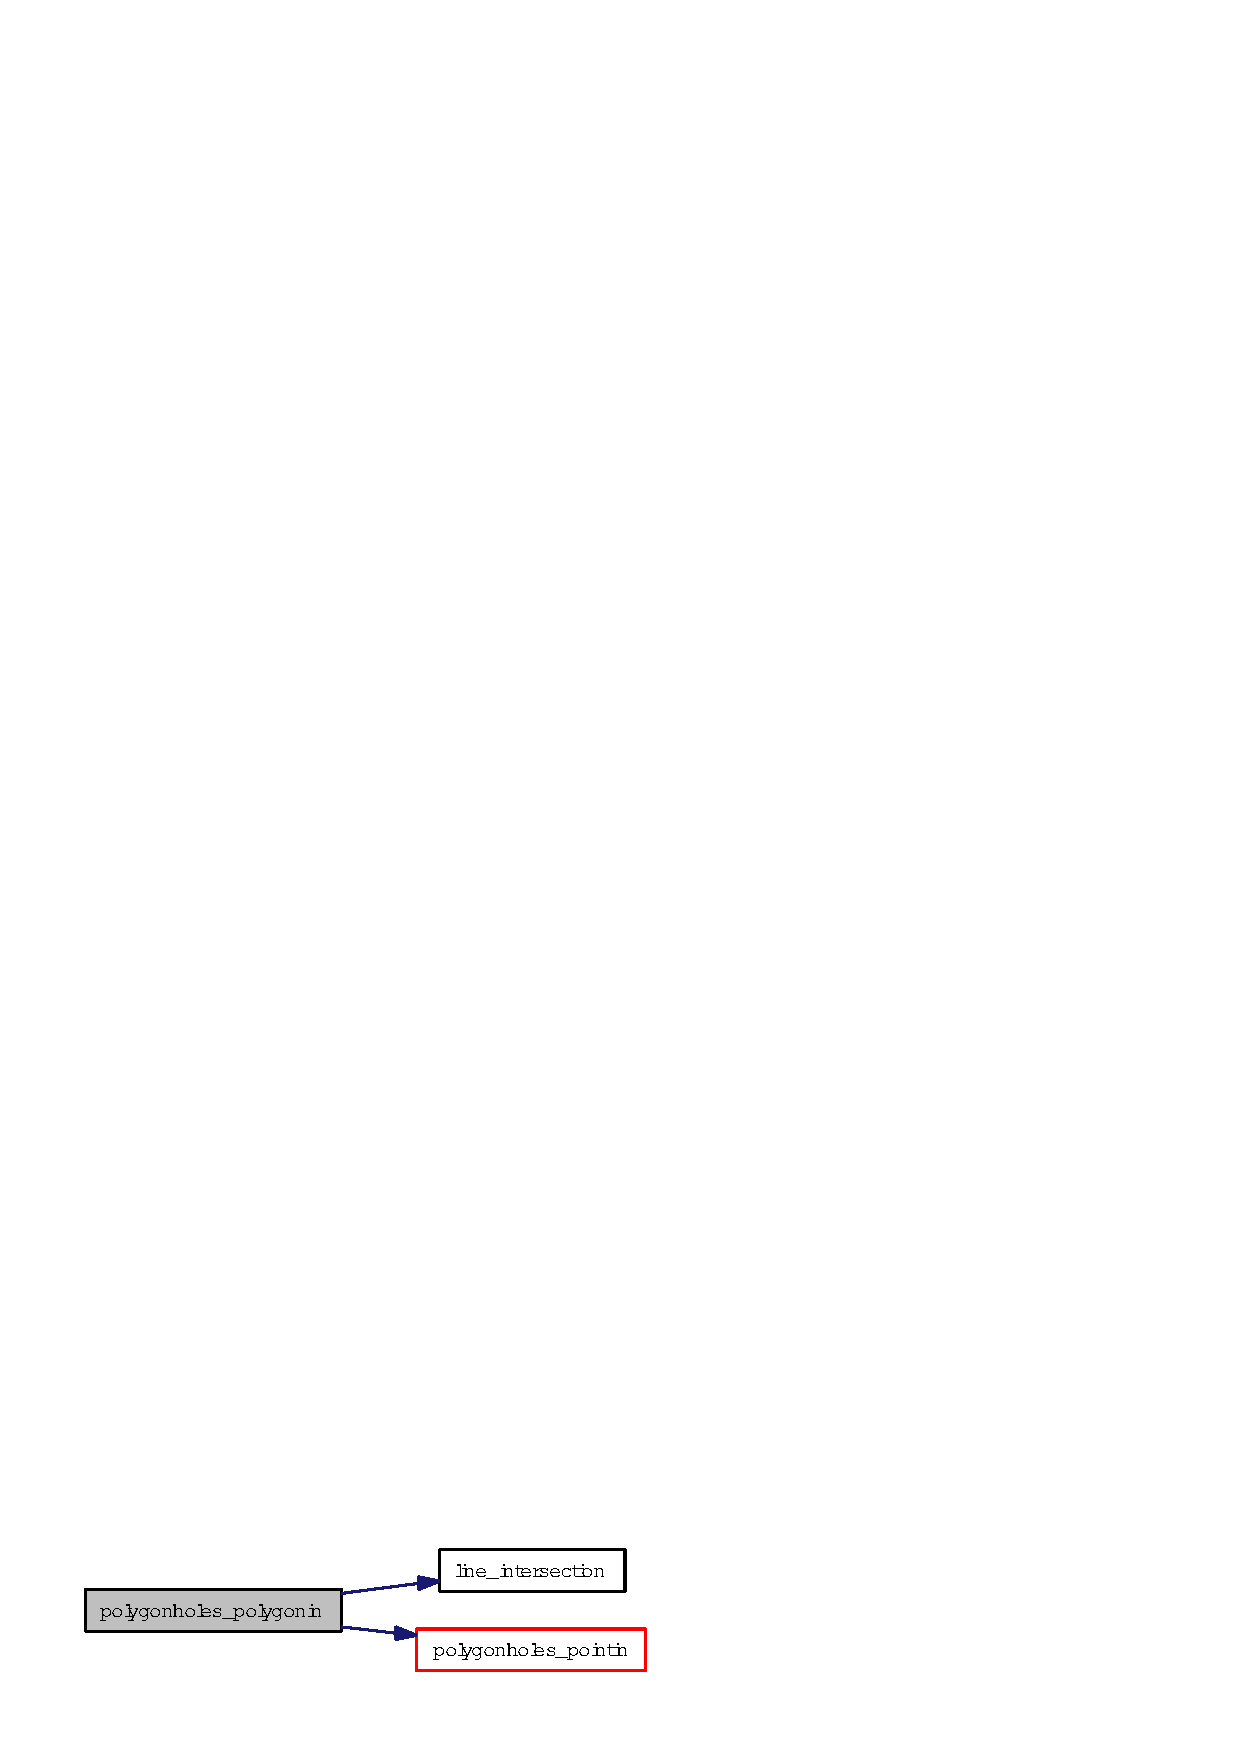
\includegraphics[width=157pt]{group__geometry_g496bae87588cb5710ced80f713da98ad_g496bae87588cb5710ced80f713da98ad_cgraph}
\end{center}
\end{figure}


Here is the caller graph for this function:\begin{figure}[H]
\begin{center}
\leavevmode
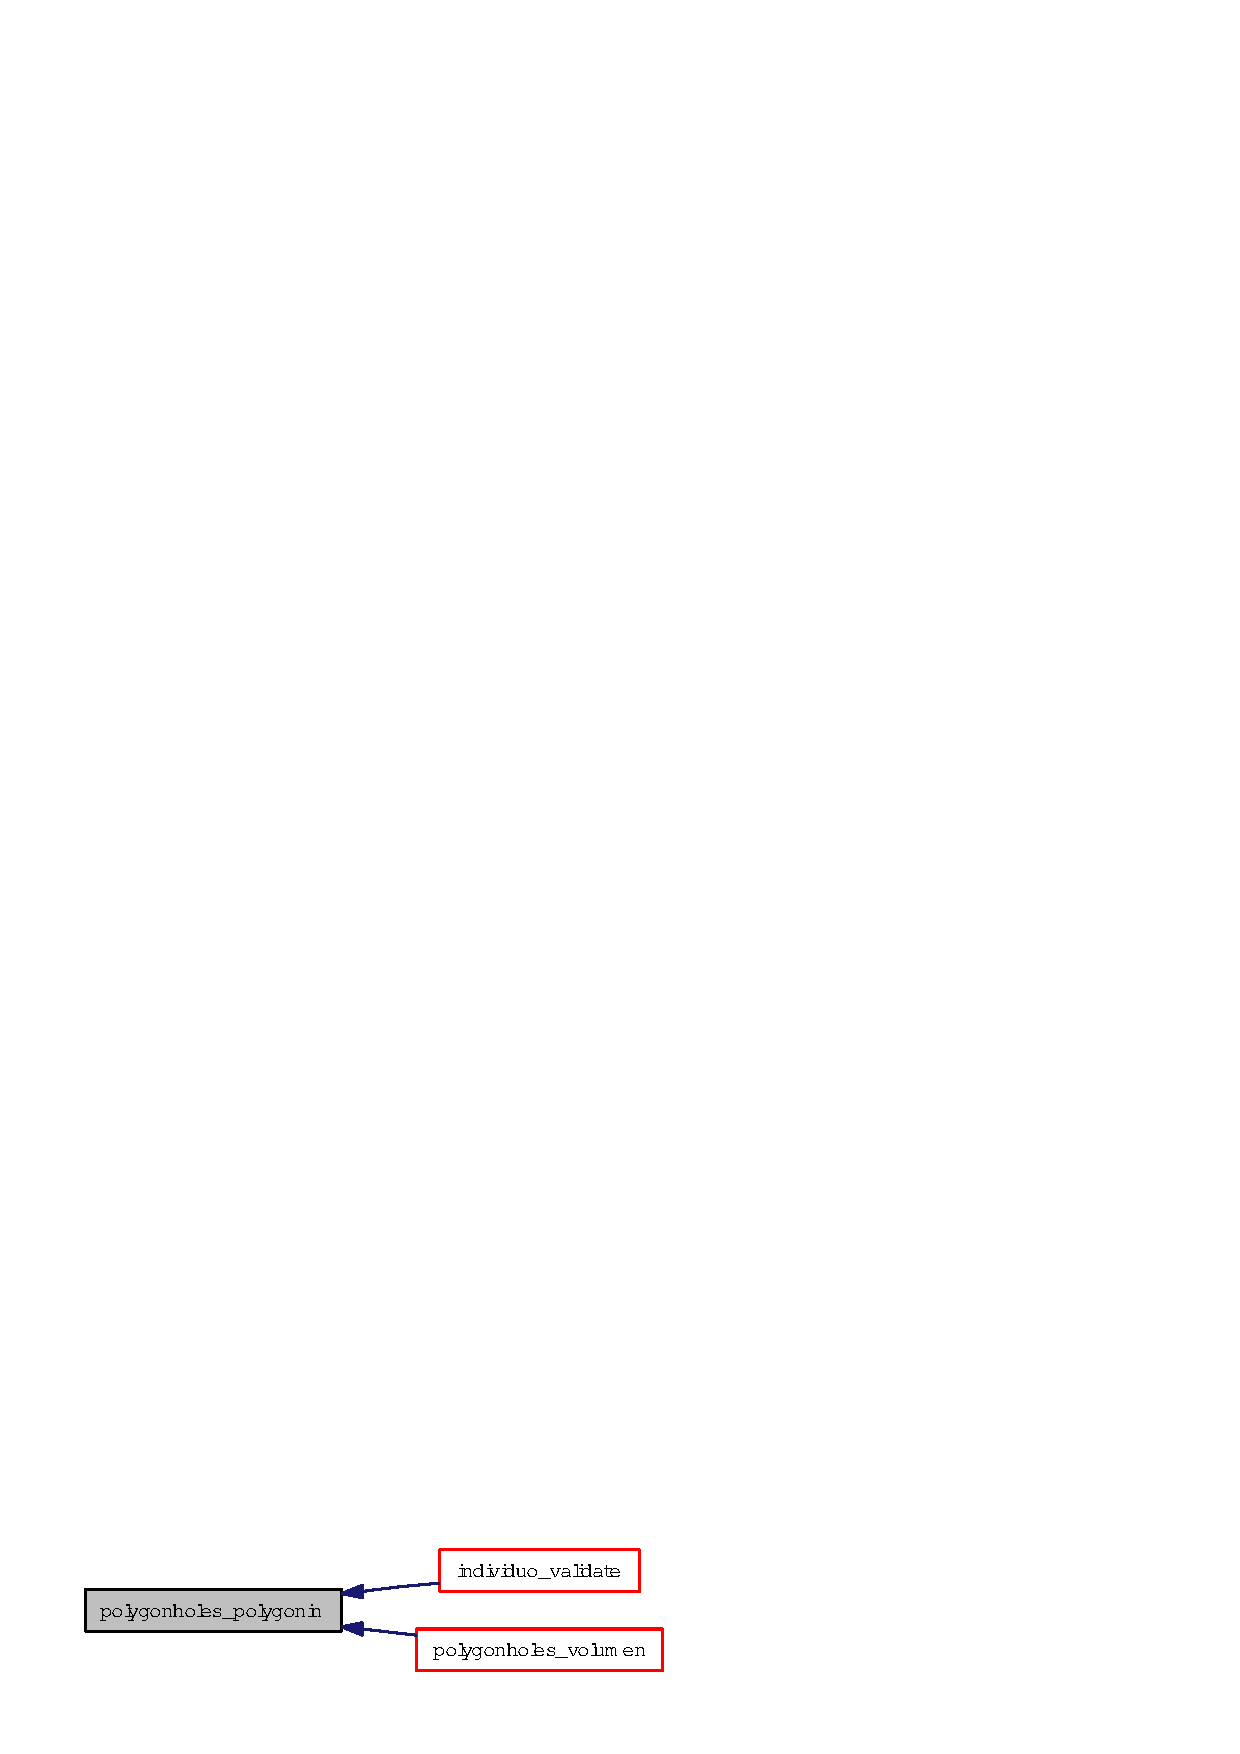
\includegraphics[width=161pt]{group__geometry_g496bae87588cb5710ced80f713da98ad_g496bae87588cb5710ced80f713da98ad_icgraph}
\end{center}
\end{figure}
\hypertarget{group__geometry_g7cf8b3f8c76179bb936754bbbf510999_g7cf8b3f8c76179bb936754bbbf510999}{
\index{geometry@{geometry}!polygonholes_volumen@{polygonholes\_\-volumen}}
\index{polygonholes_volumen@{polygonholes\_\-volumen}!geometry@{geometry}}
\subsubsection[polygonholes\_\-volumen]{\setlength{\rightskip}{0pt plus 5cm}float polygonholes\_\-volumen (\hyperlink{struct__polygon__holes}{polygon\_\-holes} $\ast$ {\em p})}}
\label{group__geometry_g7cf8b3f8c76179bb936754bbbf510999_g7cf8b3f8c76179bb936754bbbf510999}


Calcula el volumen generado por el poligono con huecos, definiendo asi el poligono como una figura tridimensional de la siguiente manera, la base del solido esta conformada por el poligono con huecos y la altura del solido en cada punto es igual a la distancia del punto a uno de los bordes.

El metodo para calcular el volumen se basa en encerrar el poligono en un rectangulo que lo contenga, y sucesivamente partir el poligono en dos subrectangulos respecto al lado mas largo calculando el volumen de cada uno de los subrectangulos y sumando el valor y esto se hace de manera recursiva.

\begin{itemize}
\item Cuando el subrectangulo esta completamente fuera del poligono no calculamos el volumen y regresamos un valor de 0\end{itemize}


\begin{itemize}
\item Cuando el subrectangulo tiene un area muy pequena definida por un da se calcula el centro del subrectangulo y se verifica que este dentro del poligono, si este es el caso, entonces se devuelve el valor del area multiplicada por la distancia del punto medio al borde, si el punto medio es 0 se devuelve 0.\end{itemize}


\begin{itemize}
\item Cuando el subrectangulo esta dentro del poligono y los vertices de este tienen su menor distancia respecto a un mismo segmento de recta se calcula el volumen del poliedro formado como el promedio de las distancias de los vertices multiplicados por el area del subrectangulo.\end{itemize}


\begin{itemize}
\item Cuando el subrectangulo esta dentro del poligono y los vertices de este tienen su menor distancia respecto a un mismo punto, que se da en el caso de los poligonos concavos, entonces se calcula el volumen como el volumen formado por la interseccion entre el cono que genera el punto y el subrectangulo, la formula que da este volumen es: $\int_{a}^{b}\int_{c}^{d}\sqrt{((x-h)^2 + (y-k)^2)} dx dy$ donde $(h,k)$ son las coordenadas del punto con respecto al que se toma la distancia, $(a,b)$ son los valores en que se desplaza $y$, $(c,d)$ son los valores en que se desplaza $x$.\end{itemize}


Esta funcion evalua menos puntos si en ves de dividir el rectangulo en 2 segun su lado mas largo, se divide en 4 partes iguales, pero esta aproximacion puede tener problemas cuando la proporcion del los lados del subrectangulo es muy grande.

\begin{Desc}
\item[Par\'{a}metros:]
\begin{description}
\item[\mbox{$\leftarrow$} {\em p}]Poligono simple con huecos en 2 dimensiones \end{description}
\end{Desc}
\begin{Desc}
\item[Devuelve:]Volumen generado \end{Desc}


\begin{Desc}
\item[\hyperlink{bug__bug000001}{Bug}]Esta funcion para calcular el volument de un rectangulo que intersecta un cono tiene valores indeterminados en algunos segmentos del problema, es posible que este error aparesca solo en algunos casos, pero hay que examinar mas la funcion. \end{Desc}


Definici\'{o}n en la l\'{\i}nea 86 del archivo polygon\_\-holes.c.

\begin{Code}\begin{verbatim}87 {
88 #if graphics
89     void draw_polygon(polygon *p)
90     {
91         int i;
92         for (i=0;i<p->nvertices;i++)
93         {
94             draw_line(p->v[i].x,p->v[i].y,p->v[(i+1)%p->nvertices].x,p->v[(i+1)%p->nvertices].y);
95         }
96     }
97 #endif
98 
99     float polygonholes_volumen_box( polygon_holes *p,
100                                     float minx,
101                                     float miny,
102                                     float maxx,
103                                     float maxy)
104     {
105 
106         float vol=0;
107         float da;
108 
109         polygon rec;
110         point q[4];
111 
112         q[0].x = minx;
113         q[0].y = miny;
114 
115         q[1].x = maxx;
116         q[1].y = miny;
117 
118         q[2].x = maxx;
119         q[2].y = maxy;
120 
121         q[3].x = minx;
122         q[3].y = maxy;
123 
124         rec.v =(point *) &q;
125         rec.nvertices = 4;
126 
127         da = polygon_area(&rec);
128 
129 
130         if (!polygon_overlapping(p->p, &rec)) //OK
131         {
132             vol = 0;
133 #if graphics
134 
135             draw_rect(minx, miny, maxx, maxy,255,255,255);
136 #endif
137 
138         }
139         else if (da < DELTA) // OK
140         {
141             point pm;
142 
143             pm.x=minx+((maxx-minx)/2.0);
144             pm.y=miny+((maxy-miny)/2.0);
145 
146             if (polygonholes_pointin(p, &pm))
147             {
148                 vol = da * distance_pointpolygonholes(&pm, p,NULL);
149 #if graphics
150 
151                 draw_rect(minx, miny, maxx, maxy,128,128,128);
152 #endif
153 
154             }
155             else
156             {
157                 vol = 0;
158 #if graphics
159 
160                 draw_rect(minx, miny, maxx, maxy,225,255,255);
161 #endif
162 
163             }
164         }
165         else
166         {
167 
168             int i;
169             float dis[4];
170             line ref[4];
171             for (i=0;i<4;i++)
172             {
173                 dis[i]=distance_pointpolygonholes(&q[i], p,&ref[i]);
174             }
175 
176             if( polygonholes_polygonin(p, &rec)
177                     &&
178                     (line_equal(&ref[0],&ref[1]) &&
179                      line_equal(&ref[1],&ref[2]) &&
180                      line_equal(&ref[2],&ref[3]))
181 
182               ) // OK
183             {
184                 if (line_ispoint(&ref[0]))// Si es un punto entonces se utiliza la formula del cono
185                 {
186                     double a,b,c,d,h,k;
187                     c=minx;
188                     d=maxx;
189                     a=miny;
190                     b=maxy;
191                     h=ref[0].v1.x;
192                     k=ref[0].v1.y;
193                     /*!\bug
194                     Esta funcion para calcular el volument de un rectangulo que intersecta un
195                     cono tiene valores indeterminados en algunos segmentos del problema, es
196                     posible que este error aparesca solo en algunos casos, pero hay que examinar
197                     mas la funcion.
198                     */
199 
200                     vol = (2*a*c*sqrt(pow(-c + h,2) + pow(a - k,2))
201                            - 2*a*h*sqrt(pow(-c + h,2) + pow(a - k,2))
202                            - 2*a*d*sqrt(pow(-d + h,2) + pow(a - k,2))
203                            + 2*a*h*sqrt(pow(-d + h,2) + pow(a - k,2))
204                            - 2*b*c*sqrt(pow(-c + h,2) + pow(b - k,2))
205                            + 2*b*h*sqrt(pow(-c + h,2) + pow(b - k,2))
206                            + 2*b*d*sqrt(pow(-d + h,2) + pow(b - k,2))
207                            - 2*b*h*sqrt(pow(-d + h,2) + pow(b - k,2))
208                            - 2*c*k*sqrt(pow(-c + h,2) + pow(a - k,2))
209                            + 2*h*k*sqrt(pow(-c + h,2) + pow(a - k,2))
210                            + 2*d*k*sqrt(pow(-d + h,2) + pow(a - k,2))
211                            - 2*h*k*sqrt(pow(-d + h,2) + pow(a - k,2))
212                            + 2*c*k*sqrt(pow(-c + h,2) + pow(b - k,2))
213                            - 2*h*k*sqrt(pow(-c + h,2) + pow(b - k,2))
214                            - 2*d*k*sqrt(pow(-d + h,2) + pow(b - k,2))
215                            + 2*h*k*sqrt(pow(-d + h,2) + pow(b - k,2))
216                            - pow(a,3)*log(-c + h + sqrt(pow(-c + h,2) + pow(a - k,2)))
217                            + 3*pow(a,2)*k*log(-c + h + sqrt(pow(-c + h,2) + pow(a - k,2)))
218                            - 3*a*pow(k,2)*log(-c + h + sqrt(pow(-c + h,2) + pow(a - k,2)))
219                            + pow(k,3)*log(-c + h + sqrt(pow(-c + h,2) + pow(a - k,2)))
220                            + pow(a,3)*log(-d + h + sqrt(pow(-d + h,2) + pow(a - k,2)))
221                            - 3*pow(a,2)*k*log(-d + h + sqrt(pow(-d + h,2) + pow(a - k,2)))
222                            + 3*a*pow(k,2)*log(-d + h + sqrt(pow(-d + h,2) + pow(a - k,2)))
223                            - pow(k,3)*log(-d + h + sqrt(pow(-d + h,2) + pow(a - k,2)))
224                            + pow(b,3)*log(-c + h + sqrt(pow(-c + h,2) + pow(b - k,2)))
225                            - 3*pow(b,2)*k*log(-c + h + sqrt(pow(-c + h,2) + pow(b - k,2)))
226                            + 3*b*pow(k,2)*log(-c + h + sqrt(pow(-c + h,2) + pow(b - k,2)))
227                            - pow(k,3)*log(-c + h + sqrt(pow(-c + h,2) + pow(b - k,2)))
228                            - pow(b,3)*log(-d + h + sqrt(pow(-d + h,2) + pow(b - k,2)))
229                            + 3*pow(b,2)*k*log(-d + h + sqrt(pow(-d + h,2) + pow(b - k,2)))
230                            - 3*b*pow(k,2)*log(-d + h + sqrt(pow(-d + h,2) + pow(b - k,2)))
231                            + pow(k,3)*log(-d + h + sqrt(pow(-d + h,2) + pow(b - k,2)))
232                            + pow(c,3)*log(a + sqrt(pow(-c + h,2) + pow(a - k,2)) - k)
233                            - 3*pow(c,2)*h*log(a + sqrt(pow(-c + h,2) + pow(a - k,2)) - k)
234                            + 3*c*pow(h,2)*log(a + sqrt(pow(-c + h,2) + pow(a - k,2)) - k)
235                            - pow(h,3)*log(a + sqrt(pow(-c + h,2) + pow(a - k,2)) - k)
236                            - pow(d,3)*log(a + sqrt(pow(-d + h,2) + pow(a - k,2)) - k)
237                            + 3*pow(d,2)*h*log(a + sqrt(pow(-d + h,2) + pow(a - k,2)) - k)
238                            - 3*d*pow(h,2)*log(a + sqrt(pow(-d + h,2) + pow(a - k,2)) - k)
239                            + pow(h,3)*log(a + sqrt(pow(-d + h,2) + pow(a - k,2)) - k)
240                            - pow(c,3)*log(b + sqrt(pow(-c + h,2) + pow(b - k,2)) - k)
241                            + 3*pow(c,2)*h*log(b + sqrt(pow(-c + h,2) + pow(b - k,2)) - k)
242                            - 3*c*pow(h,2)*log(b + sqrt(pow(-c + h,2) + pow(b - k,2)) - k)
243                            + pow(h,3)*log(b + sqrt(pow(-c + h,2) + pow(b - k,2)) - k)
244                            + pow(d,3)*log(b + sqrt(pow(-d + h,2) + pow(b - k,2)) - k)
245                            - 3*pow(d,2)*h*log(b + sqrt(pow(-d + h,2) + pow(b - k,2)) - k)
246                            + 3*d*pow(h,2)*log(b + sqrt(pow(-d + h,2) + pow(b - k,2)) - k)
247                            - pow(h,3)*log(b + sqrt(pow(-d + h,2) + pow(b - k,2)) - k))/6;
248 #if graphics
249 
250                     draw_rect(minx, miny, maxx, maxy,0,128,0);
251 #endif
252 
253                 }
254                 else // Si es una linea se utiliza la formula de la cuna
255                 {
256                     vol = (dis[0]+dis[1]+dis[2]+dis[3])/4.0 * da;
257 #if graphics
258 
259                     draw_rect(minx, miny, maxx, maxy,0,0,128);
260 #endif
261 
262                 }
263             }
264             else
265             {
266                 if (!(
267                             polygonholes_pointinhole(p, &q[0]) &&
268                             polygonholes_pointinhole(p, &q[1]) &&
269                             polygonholes_pointinhole(p, &q[2]) &&
270                             polygonholes_pointinhole(p, &q[3])
271                         )) // el poligono esta dentro de p pero no en un hueco
272                 {
273                     //Opcion de corte 1
274                     /*
275                                         vol+= polygonholes_volumen_box(p, minx, miny, (minx+maxx)/2.0, (miny+maxy)/2.0);
276                                         vol+= polygonholes_volumen_box(p, (minx+maxx)/2.0, miny, maxx, (miny+maxy)/2.0);
277                                         vol+= polygonholes_volumen_box(p, minx, (miny+maxy)/2.0, (minx+maxx)/2.0, maxy);
278                                         vol+= polygonholes_volumen_box(p, (minx+maxx)/2.0, (miny+maxy)/2.0, maxx, maxy);
279                     */
280 
281                     if (maxx-minx > maxy-miny)
282                     {
283                         vol+= polygonholes_volumen_box(p, minx, miny, (minx+maxx)/2.0, maxy);
284                         vol+= polygonholes_volumen_box(p, (minx+maxx)/2.0, miny, maxx, maxy);
285                     }
286                     else
287                     {
288                         vol+= polygonholes_volumen_box(p, minx, miny, maxx, (miny+maxy)/2.0);
289                         vol+= polygonholes_volumen_box(p, minx, (miny+maxy)/2.0, maxx, maxy);
290                     }
291 
292                 }
293 #if graphics
294                 else
295                 {
296                     draw_rect(minx, miny, maxx, maxy,0,0,255);
297                 }
298 #endif
299 
300             }
301         }
302         if (isnan(vol))
303         {
304 #if graphics
305             draw_rect(minx, miny, maxx, maxy,255,0,0);
306 #endif
307 
308             fprintf(stderr,"Error: (%f, %f) (%f, %f)\n",minx,miny,maxx,maxy);
309             vol=0;
310         }
311         return vol;
312     }
313 
314     float minx, miny, maxx, maxy;
315     polygon_minbox(p->p, &minx, &miny, &maxx, &maxy);
316 
317 #if graphics
318     getscreen();
319     clearscreen();
320     draw_polygon(p->p);
321 
322     {
323         int j;
324         for (j=0;j<p->nholes;j++)
325         {
326             draw_polygon(&(p->h[j]));
327         }
328     }
329     relscreen();
330 #endif
331 
332     return polygonholes_volumen_box(p,minx,miny,maxx,maxy);
333 }
\end{verbatim}\end{Code}




Gr\'{a}fico de llamadas para esta funci\'{o}n:\begin{figure}[H]
\begin{center}
\leavevmode
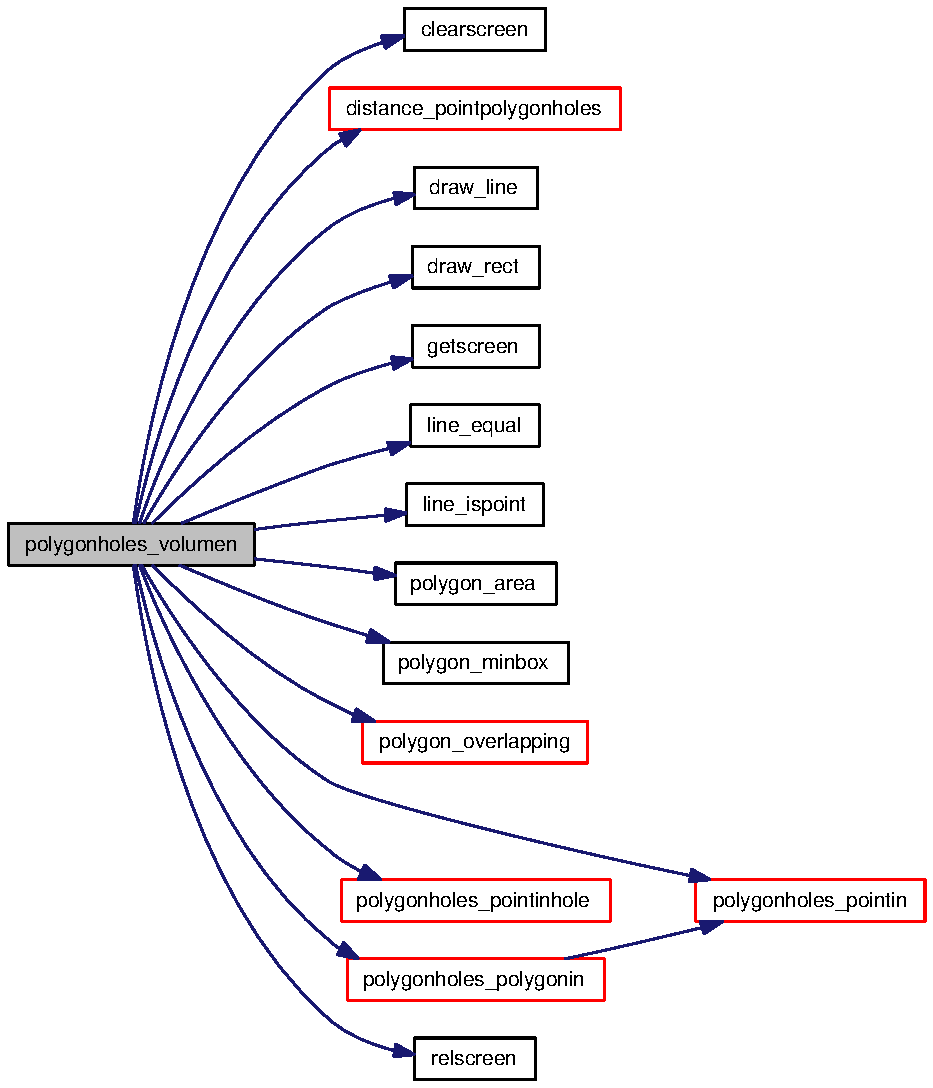
\includegraphics[width=242pt]{group__geometry_g7cf8b3f8c76179bb936754bbbf510999_g7cf8b3f8c76179bb936754bbbf510999_cgraph}
\end{center}
\end{figure}


Here is the caller graph for this function:\begin{figure}[H]
\begin{center}
\leavevmode
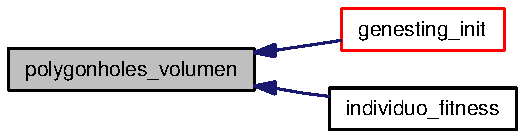
\includegraphics[width=144pt]{group__geometry_g7cf8b3f8c76179bb936754bbbf510999_g7cf8b3f8c76179bb936754bbbf510999_icgraph}
\end{center}
\end{figure}

\hypertarget{group__genetic}{
\section{Genetico}
\label{group__genetic}\index{Genetico@{Genetico}}
}


\subsection{Descripci\'{o}n detallada}
Dentro del modulo genetico encontraremos una implementacion de heuristicas de algoritmos geneticos y evoluticos que seleccionara la solucion. 

\subsection*{Archivos}
\begin{CompactItemize}
\item 
archivo \hyperlink{genesting_8h}{genesting.h}
\item 
archivo \hyperlink{individuo_8h}{individuo.h}
\item 
archivo \hyperlink{population_8h}{population.h}
\item 
archivo \hyperlink{genesting_8c}{genesting.c}
\item 
archivo \hyperlink{individuo_8c}{individuo.c}
\item 
archivo \hyperlink{population_8c}{population.c}
\end{CompactItemize}
\subsection*{Clases}
\begin{CompactItemize}
\item 
struct \hyperlink{struct__genesting}{\_\-genesting}
\item 
struct \hyperlink{struct__posicion}{\_\-posicion}
\item 
struct \hyperlink{struct__individuo}{\_\-individuo}
\item 
struct \hyperlink{struct__population}{\_\-population}
\end{CompactItemize}
\subsection*{Tipos definidos}
\begin{CompactItemize}
\item 
typedef \hyperlink{struct__genesting}{\_\-genesting} \hyperlink{group__genetic_gcd77cefe71c44c38745a4f148c7a69eb_gcd77cefe71c44c38745a4f148c7a69eb}{genesting}
\item 
typedef \hyperlink{struct__posicion}{\_\-posicion} \hyperlink{group__genetic_ge2fa8f912ec24aab702abf9b76489462_ge2fa8f912ec24aab702abf9b76489462}{posicion}
\item 
typedef \hyperlink{struct__individuo}{\_\-individuo} \hyperlink{group__genetic_g86fcc12a3e2577bedca3b8364e722da3_g86fcc12a3e2577bedca3b8364e722da3}{individuo}
\item 
typedef \hyperlink{struct__population}{\_\-population} \hyperlink{group__genetic_gdc93697b2d7197da72db59932b540a07_gdc93697b2d7197da72db59932b540a07}{population}
\end{CompactItemize}
\subsection*{Funciones}
\begin{CompactItemize}
\item 
\hyperlink{struct__genesting}{genesting} $\ast$ \hyperlink{group__genetic_g6fed4910dd1f6172bb5a4e35a97bbe56_g6fed4910dd1f6172bb5a4e35a97bbe56}{leer\_\-archivo} (char $\ast$arc\_\-name)
\item 
void \hyperlink{group__genetic_g1daa6a4e8af34b8b16a48fc2f3701f1c_g1daa6a4e8af34b8b16a48fc2f3701f1c}{genesting\_\-init} (\hyperlink{struct__genesting}{genesting} $\ast$g)
\item 
void \hyperlink{group__genetic_g3f63f4034274d731cb3fdf3200c64d41_g3f63f4034274d731cb3fdf3200c64d41}{genesting\_\-show} (\hyperlink{struct__genesting}{genesting} $\ast$g)
\item 
float \hyperlink{group__genetic_gf152bd4602acec2166cc4b91e8c8919a_gf152bd4602acec2166cc4b91e8c8919a}{individuo\_\-fitness} (\hyperlink{struct__individuo}{individuo} $\ast$ind)
\item 
void \hyperlink{group__genetic_gf4e60223d27c85a5f6166e35ecafe641_gf4e60223d27c85a5f6166e35ecafe641}{individuo\_\-create} (\hyperlink{struct__genesting}{genesting} $\ast$g, \hyperlink{struct__individuo}{individuo} $\ast$ind)
\item 
void \hyperlink{group__genetic_g05b6d3d7a4be17c9cbf479f424edd01b_g05b6d3d7a4be17c9cbf479f424edd01b}{individuo\_\-mutate} (\hyperlink{struct__individuo}{individuo} $\ast$ind)
\item 
void \hyperlink{group__genetic_g18105662f4835e24cf3b8fc40ed63b33_g18105662f4835e24cf3b8fc40ed63b33}{individuo\_\-procreate} (\hyperlink{struct__individuo}{individuo} $\ast$p, \hyperlink{struct__individuo}{individuo} $\ast$m, \hyperlink{struct__individuo}{individuo} $\ast$ind)
\item 
bool \hyperlink{group__genetic_gf80cc38ea4d590f6c45215f770d63778_gf80cc38ea4d590f6c45215f770d63778}{individuo\_\-validate} (\hyperlink{struct__individuo}{individuo} $\ast$ind)
\item 
int \hyperlink{group__genetic_gd9507b892f115e76cd4162059839370c_gd9507b892f115e76cd4162059839370c}{comparar\_\-individuos} (\hyperlink{struct__individuo}{individuo} $\ast$ind1, \hyperlink{struct__individuo}{individuo} $\ast$ind2)
\item 
void \hyperlink{group__genetic_gc7ba874876f18abab66f0a42f32b98cc_gc7ba874876f18abab66f0a42f32b98cc}{population\_\-create} (\hyperlink{struct__population}{population} $\ast$p, \hyperlink{struct__genesting}{genesting} $\ast$g, int n)
\item 
void \hyperlink{group__genetic_g229293c432c5ef4f70b1ee94c109bb1a_g229293c432c5ef4f70b1ee94c109bb1a}{population\_\-evaluate} (\hyperlink{struct__population}{population} $\ast$p)
\item 
void \hyperlink{group__genetic_g5b3202f02e14d7fb3eb1f729d1250243_g5b3202f02e14d7fb3eb1f729d1250243}{population\_\-generation} (\hyperlink{struct__population}{population} $\ast$p)
\end{CompactItemize}


\subsection{Documentaci\'{o}n de los tipos definidos}
\hypertarget{group__genetic_gcd77cefe71c44c38745a4f148c7a69eb_gcd77cefe71c44c38745a4f148c7a69eb}{
\index{genetic@{genetic}!genesting@{genesting}}
\index{genesting@{genesting}!genetic@{genetic}}
\subsubsection[genesting]{\setlength{\rightskip}{0pt plus 5cm}typedef struct \hyperlink{struct__genesting}{\_\-genesting} \hyperlink{struct__genesting}{genesting}}}
\label{group__genetic_gcd77cefe71c44c38745a4f148c7a69eb_gcd77cefe71c44c38745a4f148c7a69eb}




Definici\'{o}n en la l\'{\i}nea 25 del archivo genesting.h.\hypertarget{group__genetic_g86fcc12a3e2577bedca3b8364e722da3_g86fcc12a3e2577bedca3b8364e722da3}{
\index{genetic@{genetic}!individuo@{individuo}}
\index{individuo@{individuo}!genetic@{genetic}}
\subsubsection[individuo]{\setlength{\rightskip}{0pt plus 5cm}typedef struct \hyperlink{struct__individuo}{\_\-individuo} \hyperlink{struct__individuo}{individuo}}}
\label{group__genetic_g86fcc12a3e2577bedca3b8364e722da3_g86fcc12a3e2577bedca3b8364e722da3}




Definici\'{o}n en la l\'{\i}nea 19 del archivo individuo.h.\hypertarget{group__genetic_gdc93697b2d7197da72db59932b540a07_gdc93697b2d7197da72db59932b540a07}{
\index{genetic@{genetic}!population@{population}}
\index{population@{population}!genetic@{genetic}}
\subsubsection[population]{\setlength{\rightskip}{0pt plus 5cm}typedef struct \hyperlink{struct__population}{\_\-population} \hyperlink{struct__population}{population}}}
\label{group__genetic_gdc93697b2d7197da72db59932b540a07_gdc93697b2d7197da72db59932b540a07}




Definici\'{o}n en la l\'{\i}nea 21 del archivo population.h.\hypertarget{group__genetic_ge2fa8f912ec24aab702abf9b76489462_ge2fa8f912ec24aab702abf9b76489462}{
\index{genetic@{genetic}!posicion@{posicion}}
\index{posicion@{posicion}!genetic@{genetic}}
\subsubsection[posicion]{\setlength{\rightskip}{0pt plus 5cm}typedef struct \hyperlink{struct__posicion}{\_\-posicion} \hyperlink{struct__posicion}{posicion}}}
\label{group__genetic_ge2fa8f912ec24aab702abf9b76489462_ge2fa8f912ec24aab702abf9b76489462}




Definici\'{o}n en la l\'{\i}nea 17 del archivo individuo.h.

\subsection{Documentaci\'{o}n de las funciones}
\hypertarget{group__genetic_gd9507b892f115e76cd4162059839370c_gd9507b892f115e76cd4162059839370c}{
\index{genetic@{genetic}!comparar_individuos@{comparar\_\-individuos}}
\index{comparar_individuos@{comparar\_\-individuos}!genetic@{genetic}}
\subsubsection[comparar\_\-individuos]{\setlength{\rightskip}{0pt plus 5cm}int comparar\_\-individuos (\hyperlink{struct__individuo}{individuo} $\ast$ {\em ind1}, \hyperlink{struct__individuo}{individuo} $\ast$ {\em ind2})}}
\label{group__genetic_gd9507b892f115e76cd4162059839370c_gd9507b892f115e76cd4162059839370c}


Compara entre los dos individuos cual es mejor segun su fitness 

Definici\'{o}n en la l\'{\i}nea 275 del archivo individuo.c.

\begin{Code}\begin{verbatim}276 {
277     return ((int)(((ind1->fitness)-(ind2->fitness))*10000.0));
278 }
\end{verbatim}\end{Code}


\hypertarget{group__genetic_g1daa6a4e8af34b8b16a48fc2f3701f1c_g1daa6a4e8af34b8b16a48fc2f3701f1c}{
\index{genetic@{genetic}!genesting_init@{genesting\_\-init}}
\index{genesting_init@{genesting\_\-init}!genetic@{genetic}}
\subsubsection[genesting\_\-init]{\setlength{\rightskip}{0pt plus 5cm}void genesting\_\-init (\hyperlink{struct__genesting}{genesting} $\ast$ {\em g})}}
\label{group__genetic_g1daa6a4e8af34b8b16a48fc2f3701f1c_g1daa6a4e8af34b8b16a48fc2f3701f1c}


Realiza unas correcciones iniciales al archivo de entrada y calcula los valores fijos del problema, como el area maxima y volumen maximo que se dan cuando generamos una solucion vacia. 

Definici\'{o}n en la l\'{\i}nea 87 del archivo genesting.c.

\begin{Code}\begin{verbatim}88 {
89     int i;
90     float minx, miny, maxx, maxy;
91     polygon_holes p;
92 
93     polygon_minbox(&(g->plantilla), &minx, &miny, &maxx, &maxy);
94 
95     polygon_translate(&(g->plantilla), -minx, -miny);
96 
97     for (i=0;i<g->nhuecos;i++)
98     {
99         polygon_translate(&(g->huecos[i]), -minx, -miny);
100     }
101 
102     for (i=0;i<g->npatrones;i++)
103     {
104         polygon_minbox(&(g->patrones[i]), &minx, &miny, &maxx, &maxy);
105         polygon_translate(&(g->patrones[i]), -minx, -miny);
106     }
107 
108     p.nholes = g->nhuecos;
109     p.p = &(g->plantilla);
110     p.h = g->huecos;
111 
112     g->area = polygonholes_area(&p);
113 
114     g->volumen = polygonholes_volumen(&p);
115 }
\end{verbatim}\end{Code}




Gr\'{a}fico de llamadas para esta funci\'{o}n:\begin{figure}[H]
\begin{center}
\leavevmode
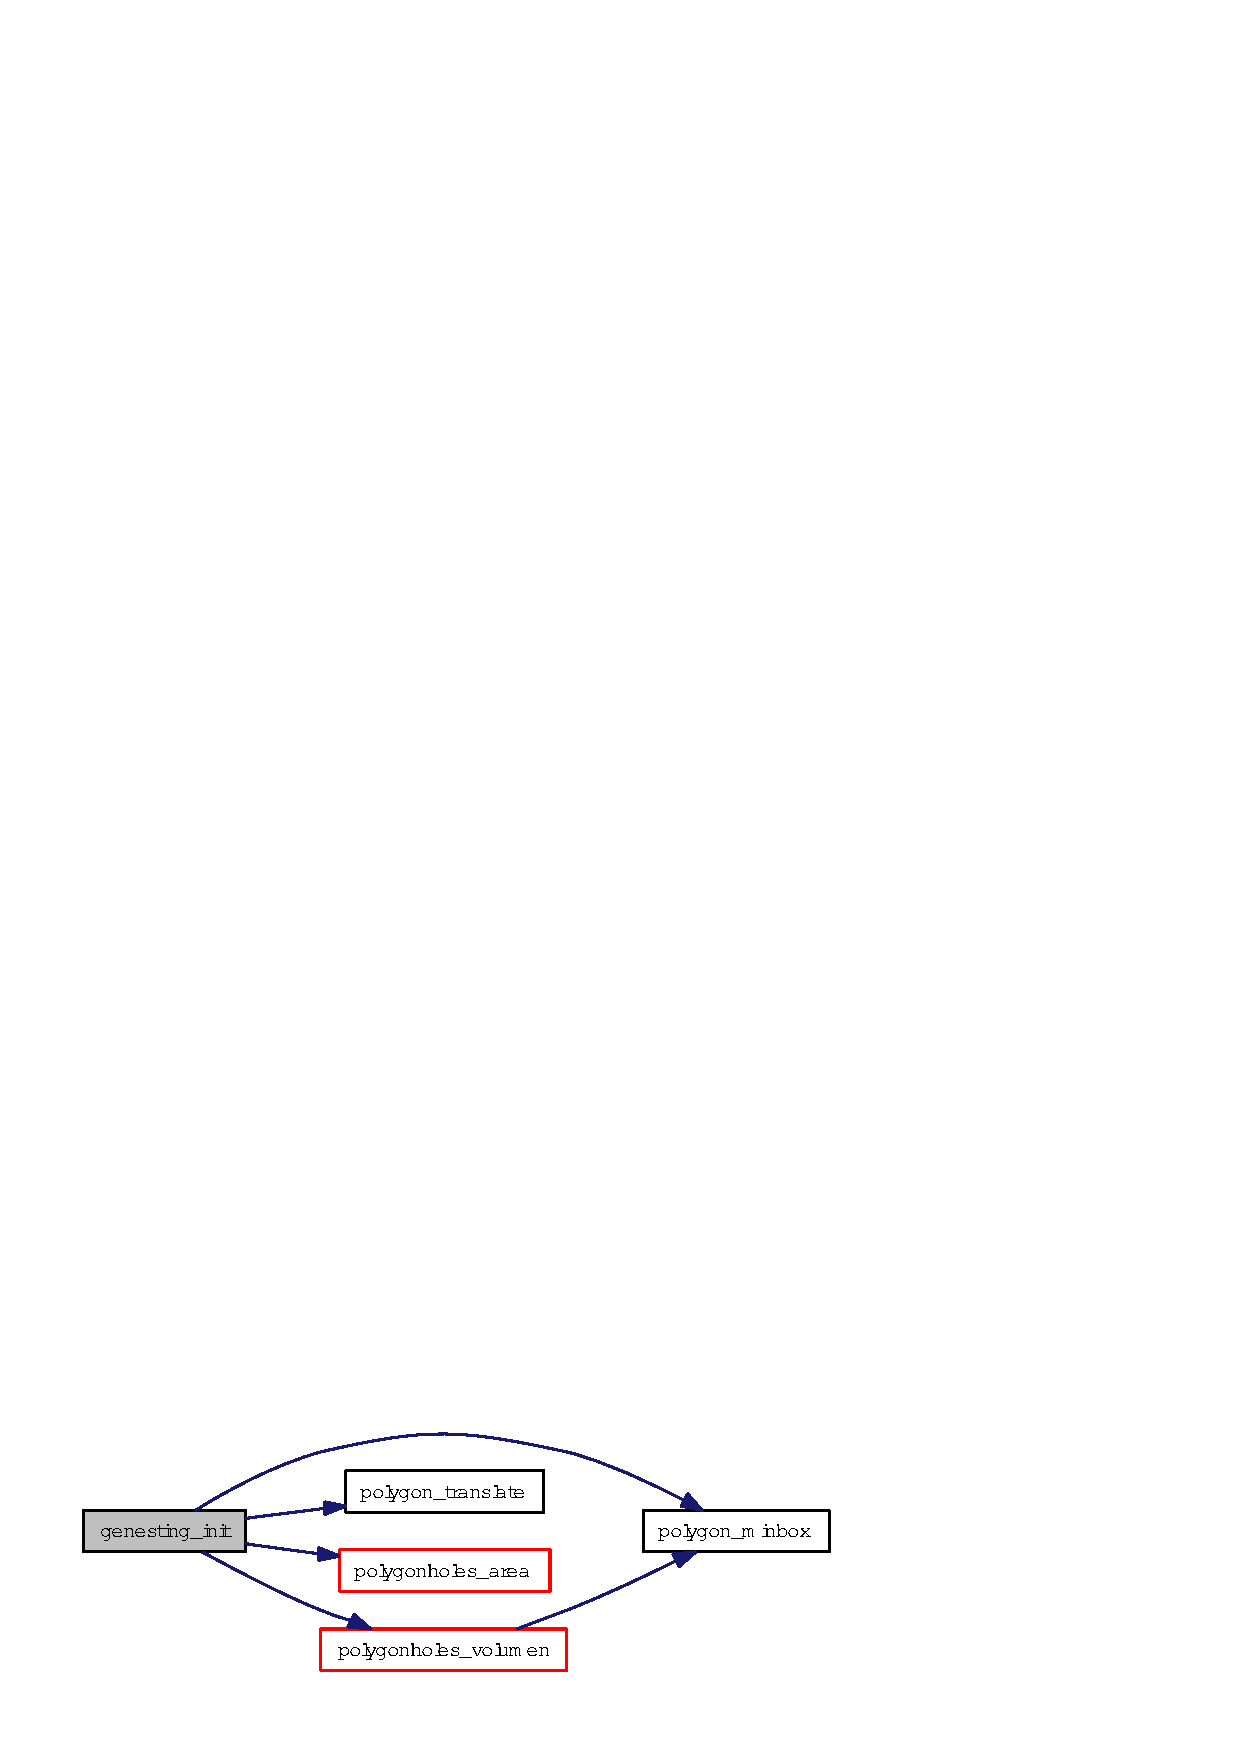
\includegraphics[width=201pt]{group__genetic_g1daa6a4e8af34b8b16a48fc2f3701f1c_g1daa6a4e8af34b8b16a48fc2f3701f1c_cgraph}
\end{center}
\end{figure}


Here is the caller graph for this function:\begin{figure}[H]
\begin{center}
\leavevmode
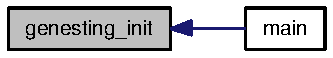
\includegraphics[width=98pt]{group__genetic_g1daa6a4e8af34b8b16a48fc2f3701f1c_g1daa6a4e8af34b8b16a48fc2f3701f1c_icgraph}
\end{center}
\end{figure}
\hypertarget{group__genetic_g3f63f4034274d731cb3fdf3200c64d41_g3f63f4034274d731cb3fdf3200c64d41}{
\index{genetic@{genetic}!genesting_show@{genesting\_\-show}}
\index{genesting_show@{genesting\_\-show}!genetic@{genetic}}
\subsubsection[genesting\_\-show]{\setlength{\rightskip}{0pt plus 5cm}void genesting\_\-show (\hyperlink{struct__genesting}{genesting} $\ast$ {\em g})}}
\label{group__genetic_g3f63f4034274d731cb3fdf3200c64d41_g3f63f4034274d731cb3fdf3200c64d41}


Muestra la informacion del programa \begin{Desc}
\item[Par\'{a}metros:]
\begin{description}
\item[\mbox{$\leftarrow$} {\em g}]Genesting \end{description}
\end{Desc}


Definici\'{o}n en la l\'{\i}nea 121 del archivo genesting.c.

\begin{Code}\begin{verbatim}122 {
123     int i;
124 
125     printf("Mostrando informacion de genesting\n");
126     printf("Plantilla:\n");
127     printf("  Vertices: %i\n",g->plantilla.nvertices);
128     printf("  Area: %f\n",polygon_area(&(g->plantilla)));
129 
130     printf("Huecos: %i\n",g->nhuecos);
131     for (i=0;i<g->nhuecos;i++)
132     {
133         printf("  Hueco %i:\n",i+1);
134         printf("    Vertices: %i\n",g->huecos[i].nvertices);
135         printf("    Area: %f\n",polygon_area(&(g->huecos[i])));
136     }
137 
138     printf("Area Util: %f\n",g->area);
139     printf("Volumen Util: %f\n",g->volumen);
140 
141     printf("Patrones: %i\n",g->npatrones);
142     for (i=0;i<g->npatrones;i++)
143     {
144         printf("  Patrones %i:\n",i+1);
145         printf("    Vertices: %i\n",g->patrones[i].nvertices);
146         printf("    Area: %f\n",polygon_area(&(g->patrones[i])));
147     }
148 }
\end{verbatim}\end{Code}




Gr\'{a}fico de llamadas para esta funci\'{o}n:\begin{figure}[H]
\begin{center}
\leavevmode
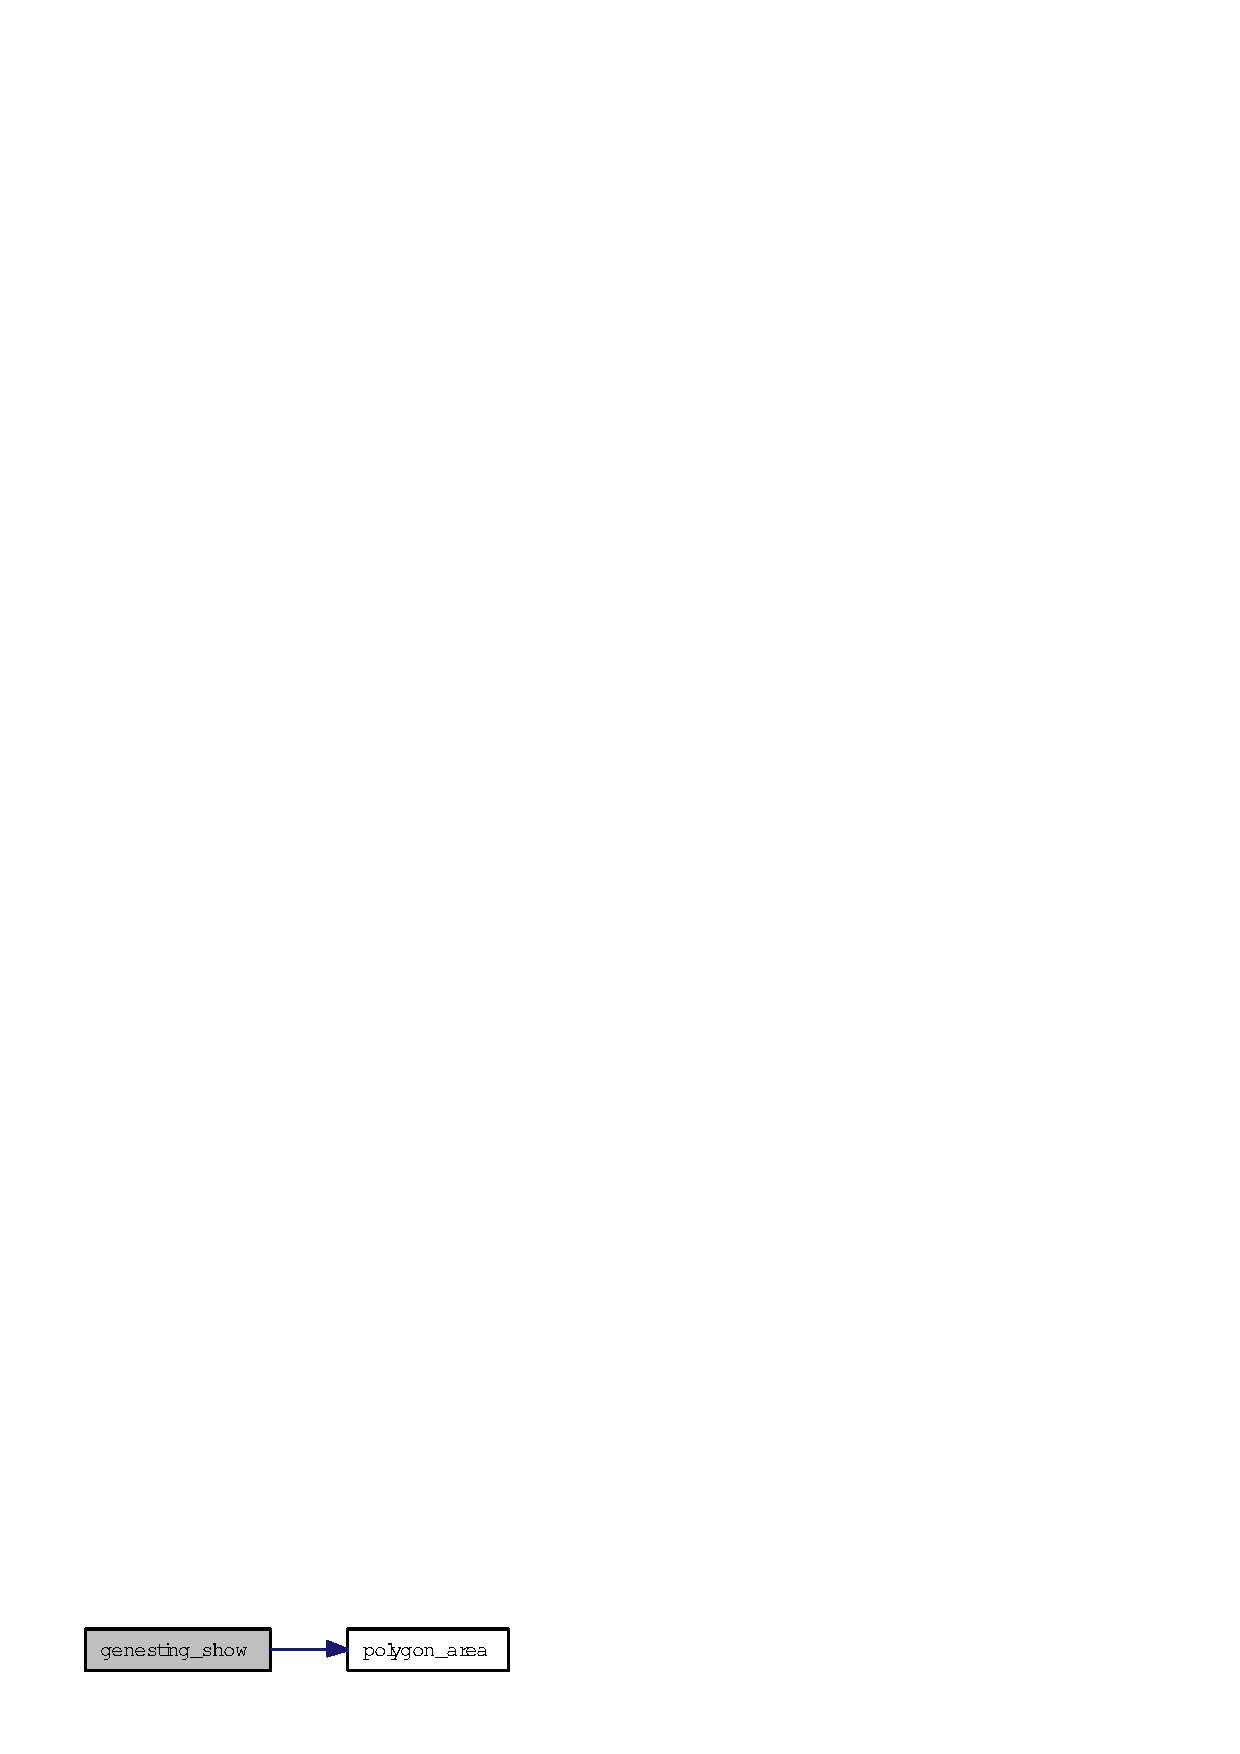
\includegraphics[width=124pt]{group__genetic_g3f63f4034274d731cb3fdf3200c64d41_g3f63f4034274d731cb3fdf3200c64d41_cgraph}
\end{center}
\end{figure}


Here is the caller graph for this function:\begin{figure}[H]
\begin{center}
\leavevmode
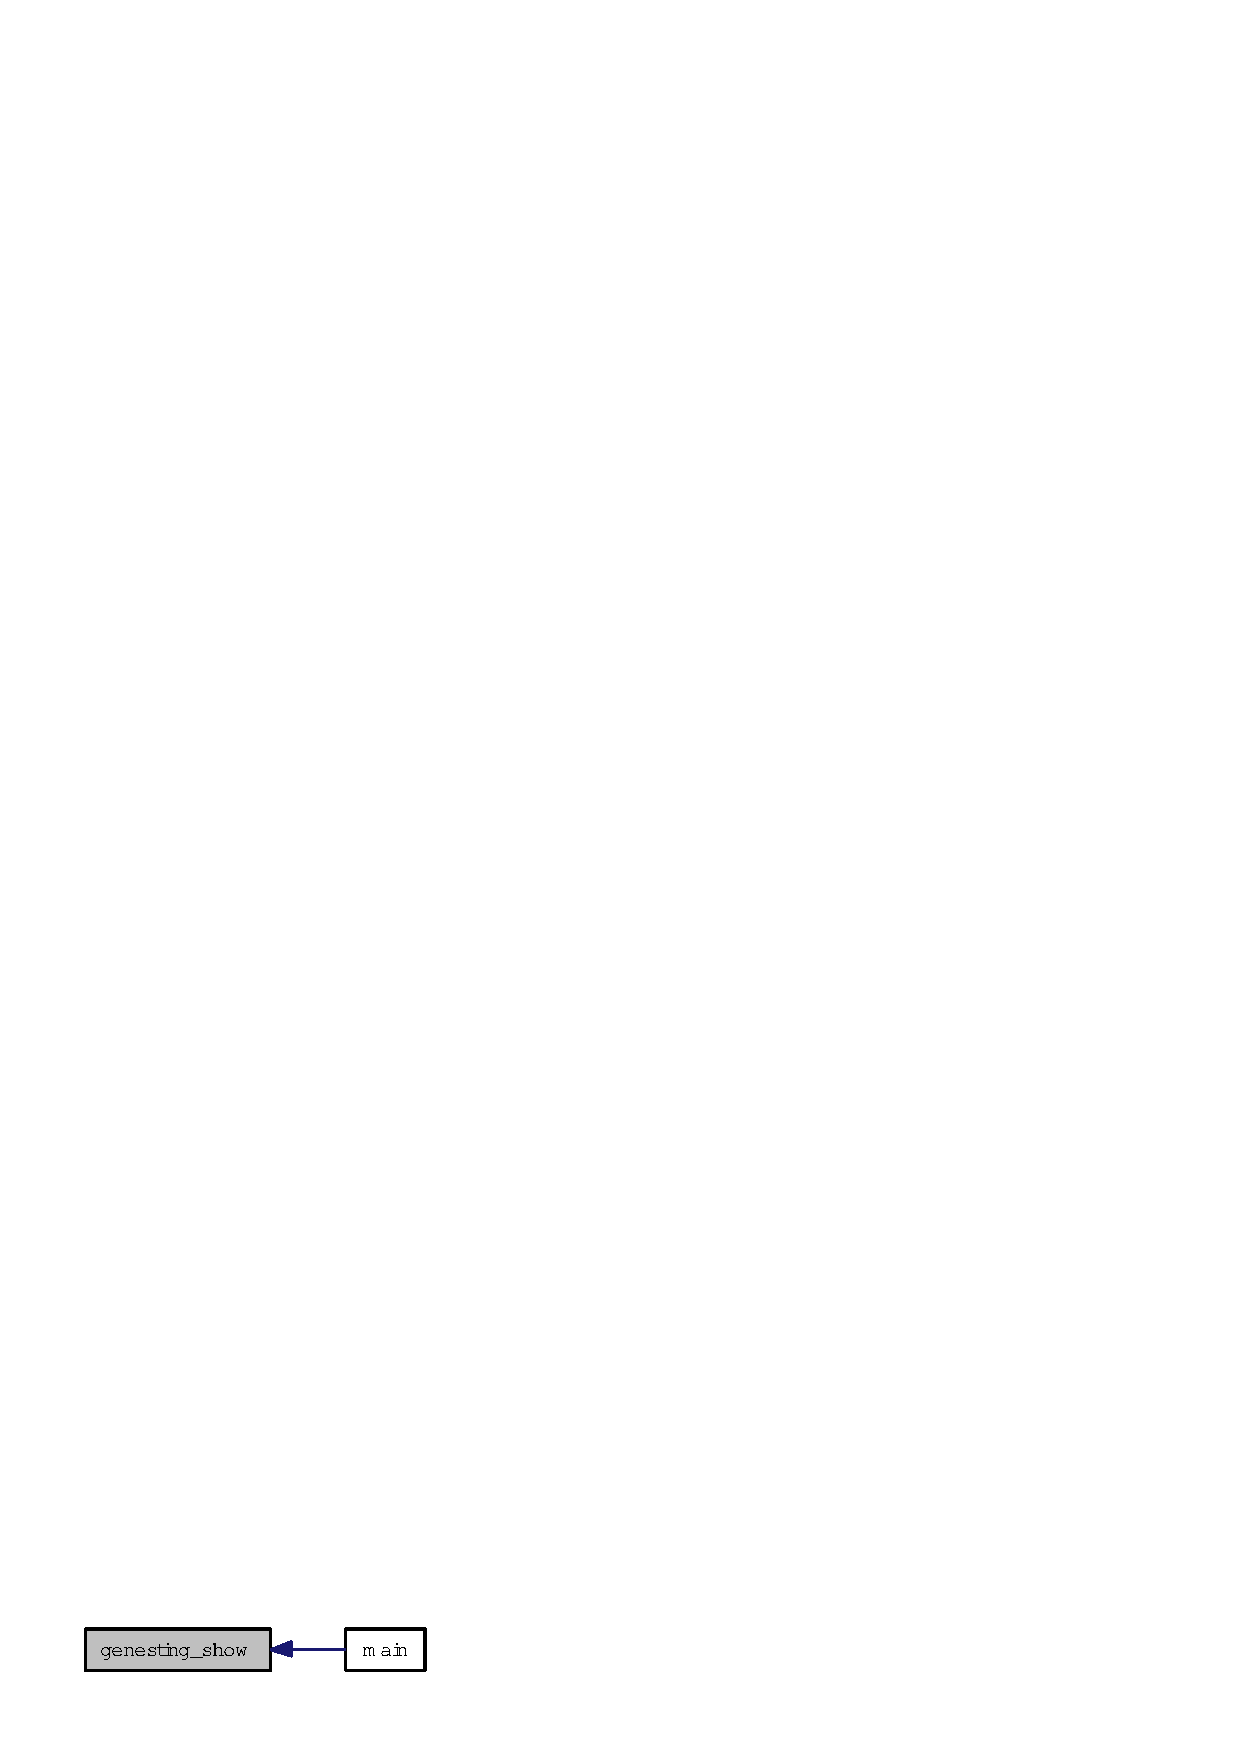
\includegraphics[width=104pt]{group__genetic_g3f63f4034274d731cb3fdf3200c64d41_g3f63f4034274d731cb3fdf3200c64d41_icgraph}
\end{center}
\end{figure}
\hypertarget{group__genetic_gf4e60223d27c85a5f6166e35ecafe641_gf4e60223d27c85a5f6166e35ecafe641}{
\index{genetic@{genetic}!individuo_create@{individuo\_\-create}}
\index{individuo_create@{individuo\_\-create}!genetic@{genetic}}
\subsubsection[individuo\_\-create]{\setlength{\rightskip}{0pt plus 5cm}void individuo\_\-create (\hyperlink{struct__genesting}{genesting} $\ast$ {\em g}, \hyperlink{struct__individuo}{individuo} $\ast$ {\em ind})}}
\label{group__genetic_gf4e60223d27c85a5f6166e35ecafe641_gf4e60223d27c85a5f6166e35ecafe641}


Esta funcion crea un individuo de configuracion aleatoria.

El individuo con el ambiente definido en el objeto genesting y en una posicion aleatoria entre el rectangulo creado por la plantilla, Ademas se selecciona solo un patron que conforma inicialmente el individuo, es posible que la configuracion obtenido genere un individuo no valido, pero esto debera ser verificado posteriormente por el algoritmo genetico.

\begin{Desc}
\item[Par\'{a}metros:]
\begin{description}
\item[\mbox{$\leftarrow$} {\em g}]Obtiene el contexto del individuo \item[\mbox{$\rightarrow$} {\em ind}]Una direccion de memoria donde esta el individuo \end{description}
\end{Desc}


Definici\'{o}n en la l\'{\i}nea 91 del archivo individuo.c.

\begin{Code}\begin{verbatim}92 {
93     float maxx,maxy,minx,miny;
94 
95     ind->ambiente = g;
96     ind->ngenes = 1;
97     ind->posgen = (posicion*) malloc (sizeof(posicion));
98     polygon_minbox(&(g->plantilla), &minx, &miny, &maxx, &maxy);
99 
100     do{
101     ind->posgen->x = (rand()%(int)(maxx-minx))+minx;
102     ind->posgen->y = (rand()%(int)(maxy-miny))+miny;
103     ind->posgen->t = (rand()%628)/100.0;
104     ind->posgen->id= rand()%g->npatrones;
105     } while (!individuo_validate(ind));
106 }
\end{verbatim}\end{Code}




Gr\'{a}fico de llamadas para esta funci\'{o}n:\begin{figure}[H]
\begin{center}
\leavevmode
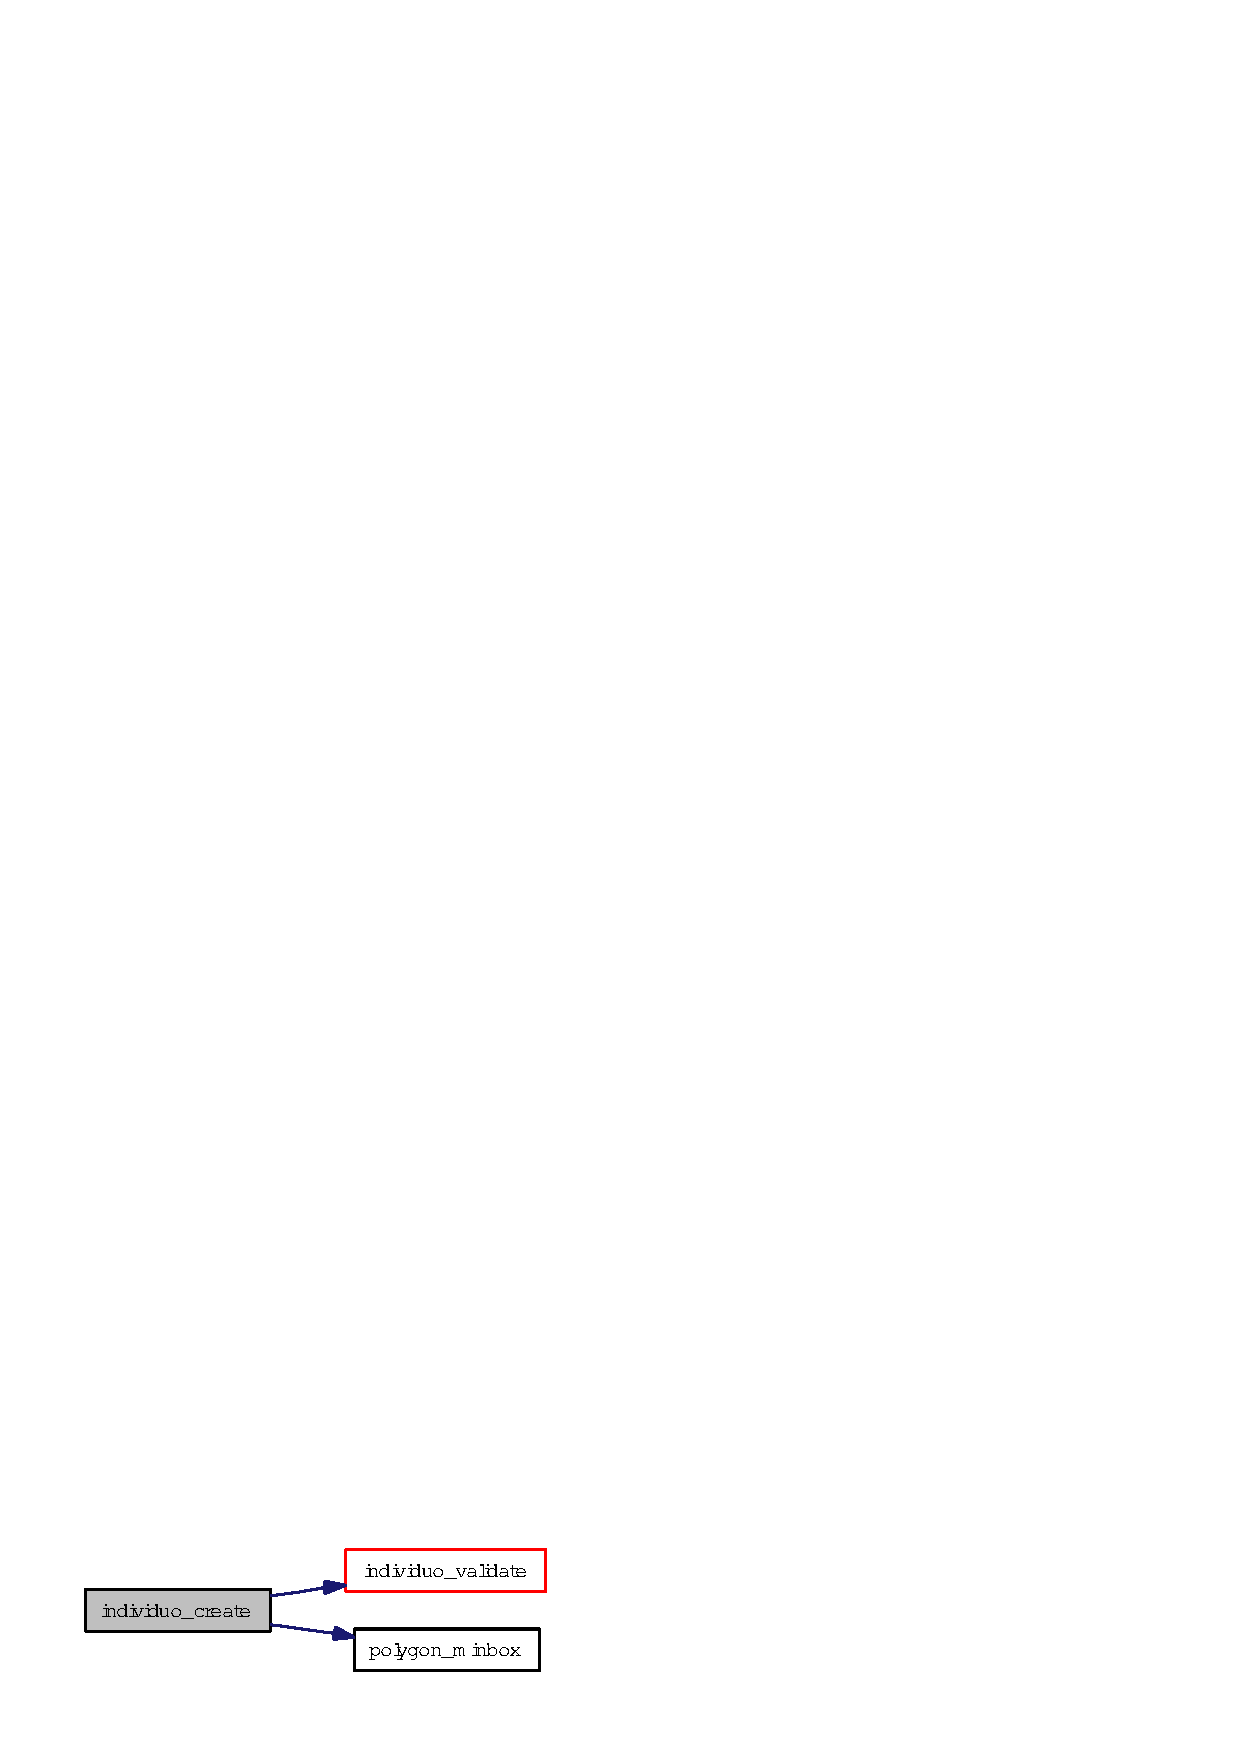
\includegraphics[width=133pt]{group__genetic_gf4e60223d27c85a5f6166e35ecafe641_gf4e60223d27c85a5f6166e35ecafe641_cgraph}
\end{center}
\end{figure}


Here is the caller graph for this function:\begin{figure}[H]
\begin{center}
\leavevmode
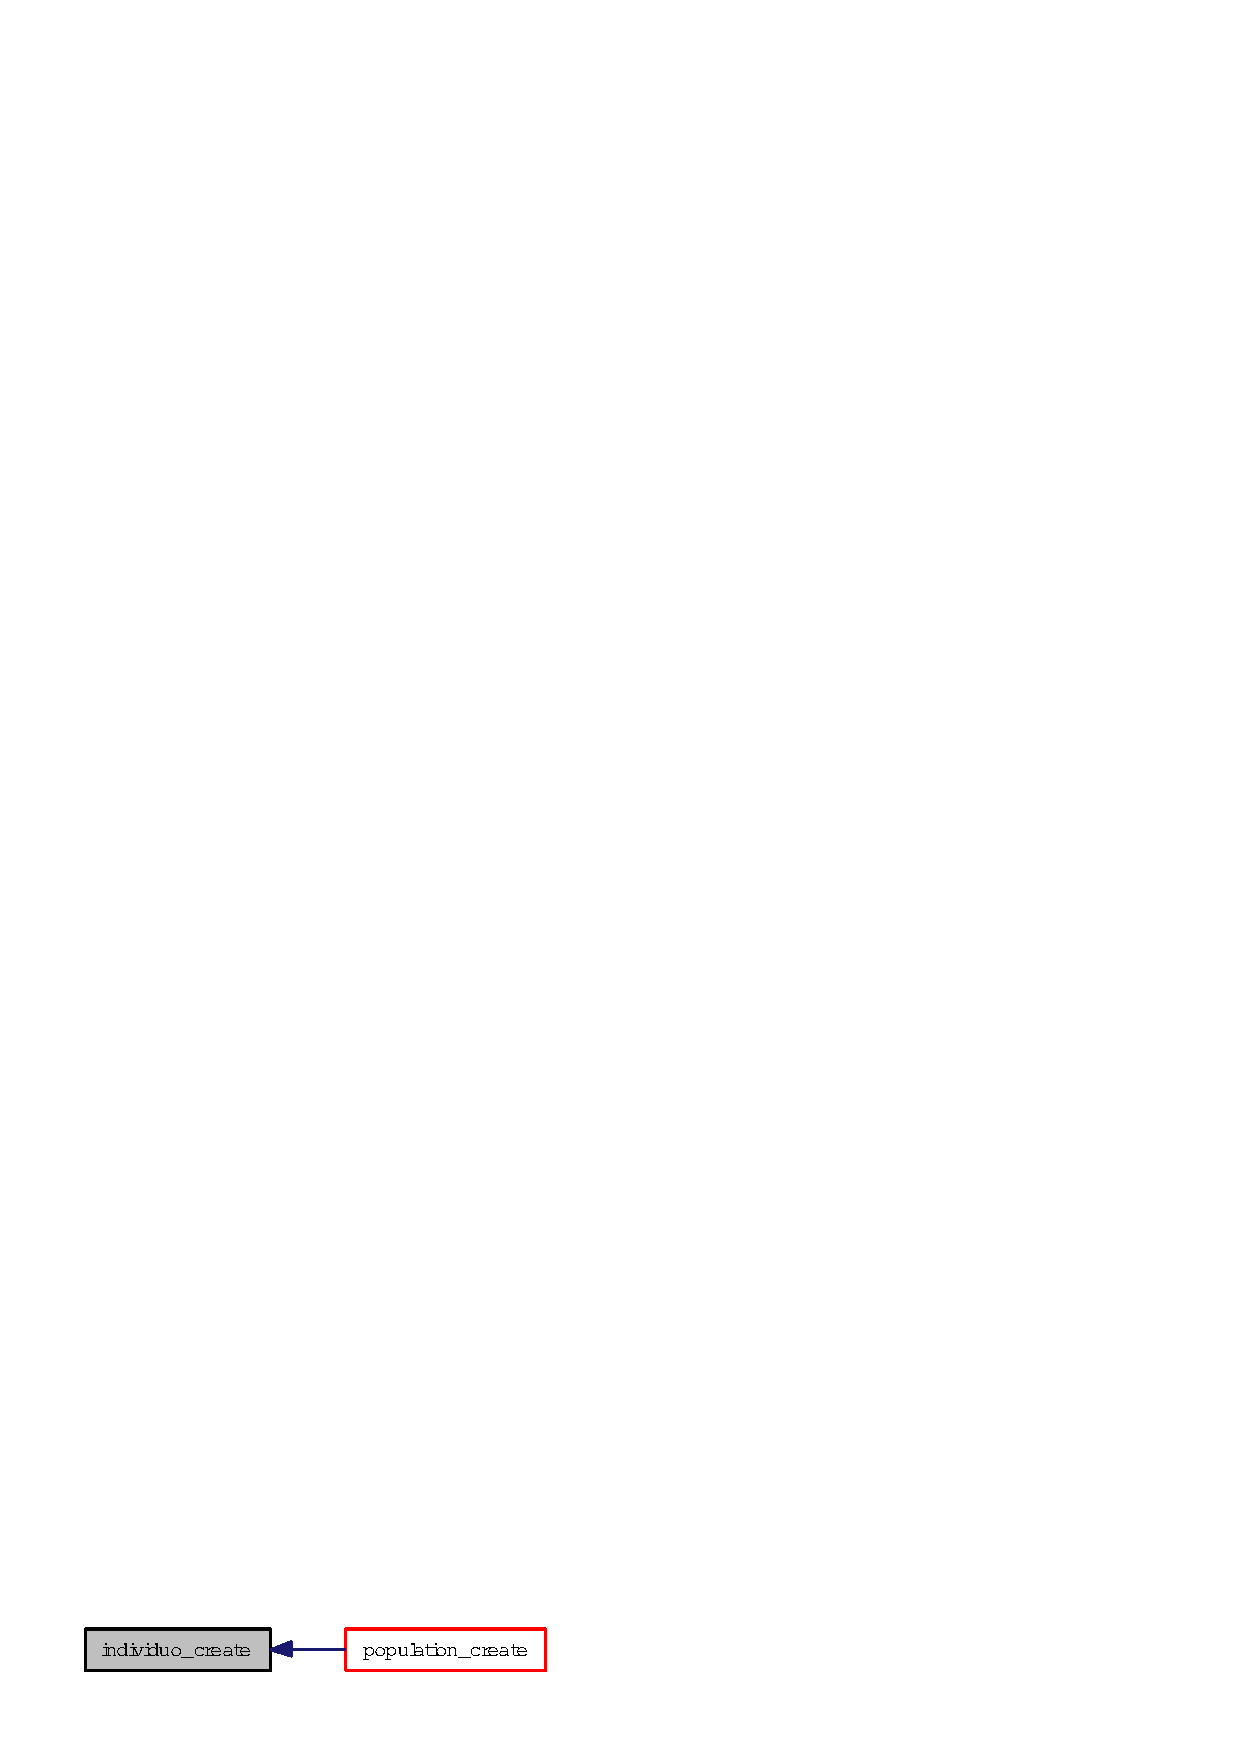
\includegraphics[width=133pt]{group__genetic_gf4e60223d27c85a5f6166e35ecafe641_gf4e60223d27c85a5f6166e35ecafe641_icgraph}
\end{center}
\end{figure}
\hypertarget{group__genetic_gf152bd4602acec2166cc4b91e8c8919a_gf152bd4602acec2166cc4b91e8c8919a}{
\index{genetic@{genetic}!individuo_fitness@{individuo\_\-fitness}}
\index{individuo_fitness@{individuo\_\-fitness}!genetic@{genetic}}
\subsubsection[individuo\_\-fitness]{\setlength{\rightskip}{0pt plus 5cm}float individuo\_\-fitness (\hyperlink{struct__individuo}{individuo} $\ast$ {\em ind})}}
\label{group__genetic_gf152bd4602acec2166cc4b91e8c8919a_gf152bd4602acec2166cc4b91e8c8919a}


\begin{Desc}
\item[\hyperlink{todo__todo000002}{Tareas Pendientes}]No es necesario recalcular el fitness de un individuo si este no ha cambiado \end{Desc}


Definici\'{o}n en la l\'{\i}nea 26 del archivo individuo.c.

\begin{Code}\begin{verbatim}27 {
28     int i,j,cont;
29 
30     polygon_holes temp;
31 
32     temp.p = &(ind->ambiente->plantilla);
33 
34     temp.h = (polygon*) malloc(sizeof(polygon)*(ind->ngenes+ind->ambiente->nhuecos));
35 
36     temp.nholes = ind->ngenes+ind->ambiente->nhuecos;
37 
38     for (i=0,cont=0;i<ind->ambiente->nhuecos;i++)
39     {
40         temp.h[cont].nvertices = ind->ambiente->huecos[i].nvertices;
41         temp.h[cont].v=(point*) malloc(sizeof(point)*temp.h[i].nvertices);
42 
43         for (j=0;j<temp.h[cont].nvertices;j++)
44         {
45             temp.h[cont].v[j].x=ind->ambiente->huecos[i].v[j].x;
46             temp.h[cont].v[j].y=ind->ambiente->huecos[i].v[j].y;
47         }
48         cont++;
49     }
50     for (i=0;i<ind->ngenes;i++)
51     {
52         temp.h[cont].nvertices = ind->ambiente->patrones[ind->posgen[i].id].nvertices;
53         temp.h[cont].v = (point*) malloc(sizeof(point)*temp.h[cont].nvertices);
54         for (j=0;j<temp.h[cont].nvertices;j++)
55         {
56             temp.h[cont].v[j].x=ind->ambiente->patrones[ind->posgen[i].id].v[j].x;
57             temp.h[cont].v[j].y=ind->ambiente->patrones[ind->posgen[i].id].v[j].y;
58         }
59         polygon_rotate(&(temp.h[cont]),ind->posgen[i].t);
60         polygon_translate(&(temp.h[cont]),ind->posgen[i].x, ind->posgen[i].y);
61         cont++;
62     }
63 
64     ind->fitness = polygonholes_volumen(&temp)/(ind->ambiente->volumen);
65 
66     ind->areautil = polygonholes_area(&temp);
67 
68     for (i=0;i<temp.nholes;i++)
69     {
70         free(temp.h[i].v);
71     }
72     free (temp.h);
73 
74     return (ind->fitness);
75 }
\end{verbatim}\end{Code}




Gr\'{a}fico de llamadas para esta funci\'{o}n:\begin{figure}[H]
\begin{center}
\leavevmode
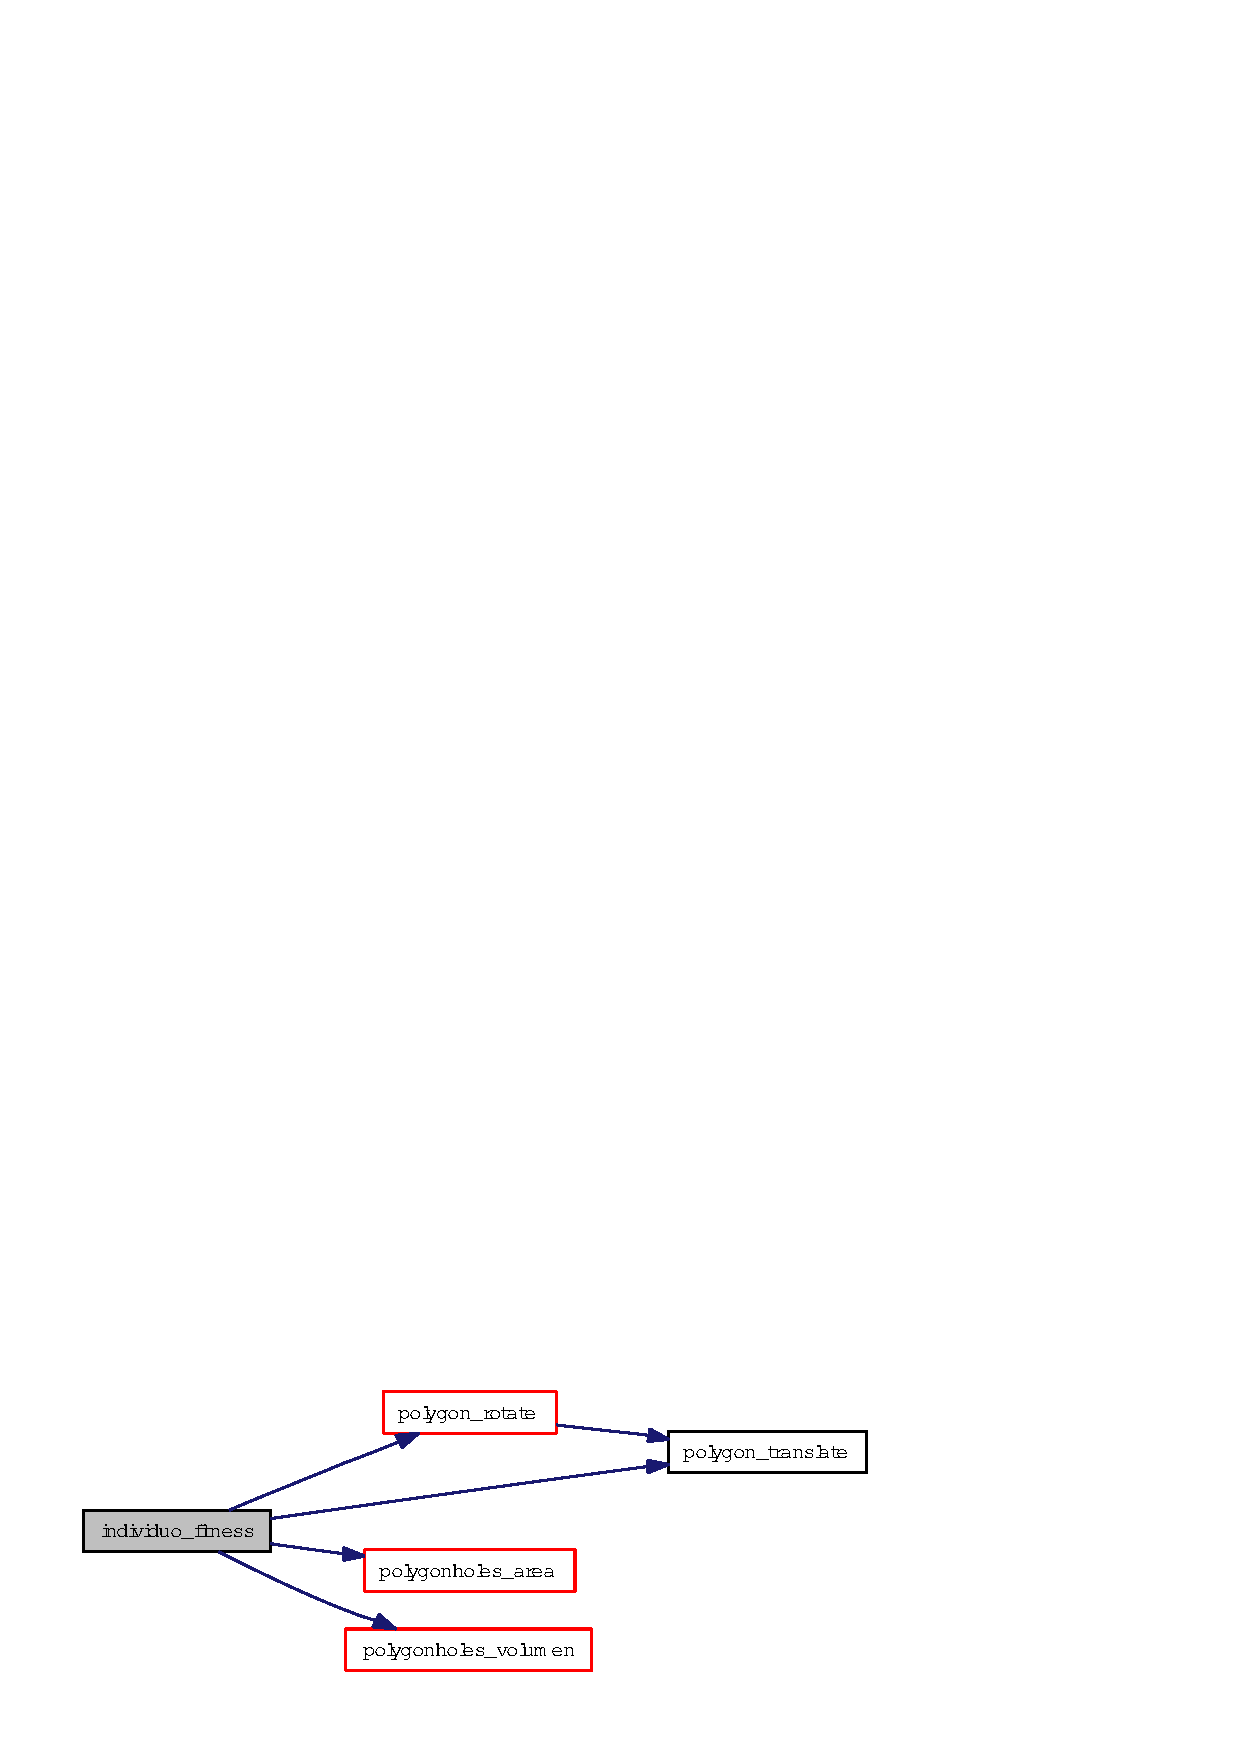
\includegraphics[width=210pt]{group__genetic_gf152bd4602acec2166cc4b91e8c8919a_gf152bd4602acec2166cc4b91e8c8919a_cgraph}
\end{center}
\end{figure}
\hypertarget{group__genetic_g05b6d3d7a4be17c9cbf479f424edd01b_g05b6d3d7a4be17c9cbf479f424edd01b}{
\index{genetic@{genetic}!individuo_mutate@{individuo\_\-mutate}}
\index{individuo_mutate@{individuo\_\-mutate}!genetic@{genetic}}
\subsubsection[individuo\_\-mutate]{\setlength{\rightskip}{0pt plus 5cm}void individuo\_\-mutate (\hyperlink{struct__individuo}{individuo} $\ast$ {\em ind})}}
\label{group__genetic_g05b6d3d7a4be17c9cbf479f424edd01b_g05b6d3d7a4be17c9cbf479f424edd01b}


Esta funcion modifica un individuo aleatoriamente.

\begin{Desc}
\item[Par\'{a}metros:]
\begin{description}
\item[\mbox{$\leftrightarrow$} {\em ind}]Individuo \end{description}
\end{Desc}


Definici\'{o}n en la l\'{\i}nea 113 del archivo individuo.c.

\begin{Code}\begin{verbatim}114 {
115     int i;
116     for (i=0;i<ind->ngenes;i++){
117         ind->posgen[i].x += (rand()%4)-2;
118         ind->posgen[i].y += (rand()%4)-2;
119         ind->posgen[i].t += ((rand()%100)-50)/100.0;
120     }
121 };
\end{verbatim}\end{Code}


\hypertarget{group__genetic_g18105662f4835e24cf3b8fc40ed63b33_g18105662f4835e24cf3b8fc40ed63b33}{
\index{genetic@{genetic}!individuo_procreate@{individuo\_\-procreate}}
\index{individuo_procreate@{individuo\_\-procreate}!genetic@{genetic}}
\subsubsection[individuo\_\-procreate]{\setlength{\rightskip}{0pt plus 5cm}void individuo\_\-procreate (\hyperlink{struct__individuo}{individuo} $\ast$ {\em p}, \hyperlink{struct__individuo}{individuo} $\ast$ {\em m}, \hyperlink{struct__individuo}{individuo} $\ast$ {\em ind})}}
\label{group__genetic_g18105662f4835e24cf3b8fc40ed63b33_g18105662f4835e24cf3b8fc40ed63b33}


Esta funcion crea un nuevo individuo partiendo de los individuos padres. La mescla se hace de la siguiente manera, se toman los patrones del padre y luego los patrones de la madre si ya no estan ya colocados, si hay patrones comunes de forma cuasi aleatoria se escoge cual de las posiciones del patron es heredada.

\begin{Desc}
\item[Par\'{a}metros:]
\begin{description}
\item[\mbox{$\leftarrow$} {\em p}]Individuo padre \item[\mbox{$\leftarrow$} {\em m}]Individuo madre \item[\mbox{$\rightarrow$} {\em ind}]Nuevo individuo \end{description}
\end{Desc}


Definici\'{o}n en la l\'{\i}nea 121 del archivo individuo.c.\hypertarget{group__genetic_gf80cc38ea4d590f6c45215f770d63778_gf80cc38ea4d590f6c45215f770d63778}{
\index{genetic@{genetic}!individuo_validate@{individuo\_\-validate}}
\index{individuo_validate@{individuo\_\-validate}!genetic@{genetic}}
\subsubsection[individuo\_\-validate]{\setlength{\rightskip}{0pt plus 5cm}bool individuo\_\-validate (\hyperlink{struct__individuo}{individuo} $\ast$ {\em ind})}}
\label{group__genetic_gf80cc38ea4d590f6c45215f770d63778_gf80cc38ea4d590f6c45215f770d63778}


Esta funcion identifica si un individuo es una solucion validad, esto es verdadero si se cumplen las siguientes condiciones:\begin{itemize}
\item No se repite ningun patron dentro de la solucion\item Todos los patrones estan dentro de la plantilla\item Ningun patron se solapa con la plantilla, huecos u otro patron En caso contrario el individuo no es valido.\end{itemize}


\begin{Desc}
\item[Par\'{a}metros:]
\begin{description}
\item[\mbox{$\leftarrow$} {\em ind}]Individuo a validar \end{description}
\end{Desc}
\begin{Desc}
\item[Devuelve:]Verdadero si es un individuo valido, falso en caso contrario. \end{Desc}


Definici\'{o}n en la l\'{\i}nea 190 del archivo individuo.c.

\begin{Code}\begin{verbatim}191 {
192     bool valido = true;
193     int i,j;
194     polygon_holes ph;
195     polygon *pat;
196 
197     for (i=0;i<ind->ngenes-1 && valido;i++)
198     {
199         for (j=i+1;j<ind->ngenes && valido;j++)
200         {
201             if (ind->posgen[i].id == ind->posgen[j].id)
202                 valido = false;
203         }
204     }
205 
206     ph.p = &(ind->ambiente->plantilla);
207     ph.nholes = ind->ambiente->nhuecos;
208     ph.h = (polygon*) malloc(sizeof(polygon)*ph.nholes);
209 
210     for (i=0;i<ph.nholes;i++)
211     {
212         ph.h[i].nvertices = ind->ambiente->huecos[i].nvertices;
213         ph.h[i].v=(point*) malloc(sizeof(point)*ph.h[i].nvertices);
214 
215         for (j=0;j<ph.h[i].nvertices;j++)
216         {
217             ph.h[i].v[j].x=ind->ambiente->huecos[i].v[j].x;
218             ph.h[i].v[j].y=ind->ambiente->huecos[i].v[j].y;
219         }
220     }
221 
222     pat = (polygon*) malloc(sizeof(polygon)*ind->ngenes);
223 
224     for (i=0;i<ind->ngenes;i++)
225     {
226         pat[i].nvertices = ind->ambiente->patrones[ind->posgen[i].id].nvertices;
227         pat[i].v = (point*) malloc(sizeof(point)*pat[i].nvertices);
228         for (j=0;j<pat[i].nvertices;j++)
229         {
230             pat[i].v[j].x=ind->ambiente->patrones[ind->posgen[i].id].v[j].x;
231             pat[i].v[j].y=ind->ambiente->patrones[ind->posgen[i].id].v[j].y;
232         }
233         polygon_rotate(&(pat[i]),ind->posgen[i].t);
234         polygon_translate(&(pat[i]),ind->posgen[i].x, ind->posgen[i].y);
235     }
236 
237     for (i=0;i<ind->ngenes && valido;i++)
238     {
239         if(!polygonholes_polygonin(&ph, &(pat[i])))
240         {
241             valido=false;
242         }
243     }
244 
245     for (i=0;i<ind->ngenes-1 && valido;i++)
246     {
247         for (j=i+1;j<ind->ngenes && valido;j++)
248         {
249             if (polygon_overlapping(&(pat[i]),&(pat[j])))
250             {
251                 valido=false;
252             }
253         }
254     }
255 
256     for (i=0;i<ind->ngenes;i++)
257     {
258         free(pat[i].v);
259     }
260     free(pat);
261 
262     for (i=0;i<ph.nholes;i++)
263     {
264         free(ph.h[i].v);
265     }
266     free(ph.h);
267 
268     return valido;
269 }
\end{verbatim}\end{Code}




Gr\'{a}fico de llamadas para esta funci\'{o}n:\begin{figure}[H]
\begin{center}
\leavevmode
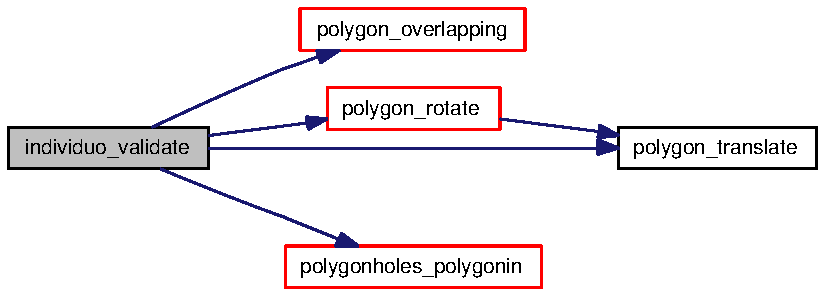
\includegraphics[width=216pt]{group__genetic_gf80cc38ea4d590f6c45215f770d63778_gf80cc38ea4d590f6c45215f770d63778_cgraph}
\end{center}
\end{figure}


Here is the caller graph for this function:\begin{figure}[H]
\begin{center}
\leavevmode
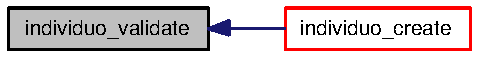
\includegraphics[width=133pt]{group__genetic_gf80cc38ea4d590f6c45215f770d63778_gf80cc38ea4d590f6c45215f770d63778_icgraph}
\end{center}
\end{figure}
\hypertarget{group__genetic_g6fed4910dd1f6172bb5a4e35a97bbe56_g6fed4910dd1f6172bb5a4e35a97bbe56}{
\index{genetic@{genetic}!leer_archivo@{leer\_\-archivo}}
\index{leer_archivo@{leer\_\-archivo}!genetic@{genetic}}
\subsubsection[leer\_\-archivo]{\setlength{\rightskip}{0pt plus 5cm}\hyperlink{struct__genesting}{genesting} $\ast$ leer\_\-archivo (char $\ast$ {\em arc\_\-name})}}
\label{group__genetic_g6fed4910dd1f6172bb5a4e35a97bbe56_g6fed4910dd1f6172bb5a4e35a97bbe56}


\begin{Desc}
\item[\hyperlink{todo__todo000001}{Tareas Pendientes}]Documentar como es la estructura leida por el programa. \end{Desc}


Definici\'{o}n en la l\'{\i}nea 25 del archivo genesting.c.

\begin{Code}\begin{verbatim}26 {
27     FILE* arc;
28     genesting *g;
29     int npoly;
30     int i,j;
31 
32     g =(genesting*) malloc (sizeof(genesting));
33 
34     arc=fopen(arc_name,"r");
35 
36     if(arc==NULL){
37             fprintf(stderr,"No se pudo abrir el archivo\n");
38             exit(1);
39     }
40 
41     fscanf(arc,"%i",&npoly);
42 
43     g->nhuecos =0;
44     g->npatrones =0;
45 
46     g->huecos=(polygon*) malloc(sizeof(polygon)*npoly-1);
47     g->patrones=(polygon*) malloc(sizeof(polygon)*npoly-1);
48 
49     for (i=0;i<npoly;i++)
50     {
51         int nvert,tipo;
52 
53         polygon *p=NULL;
54         fscanf(arc,"%i %i",&nvert,&tipo);
55         switch(tipo)
56         {
57             case 1:
58             p=&(g->plantilla);
59             break;
60             case 2:
61             p=&(g->patrones[g->npatrones++]);
62             break;
63             case 3:
64             p=&(g->huecos[g->nhuecos++]);
65             break;
66         }
67         p->nvertices = nvert;
68         p->v=(point*) malloc(sizeof(point)*nvert);
69         for (j=0;j<nvert;j++)
70         {
71             fscanf(arc,"%f %f",&(p->v[j].x),&(p->v[j].y));
72         }
73     }
74     g->huecos=(polygon*) realloc(g->huecos,sizeof(polygon)*g->nhuecos);
75     g->patrones=(polygon*) realloc(g->patrones,sizeof(polygon)*g->npatrones);
76 
77     fclose(arc);
78 
79     return g;
80 }
\end{verbatim}\end{Code}




Here is the caller graph for this function:\begin{figure}[H]
\begin{center}
\leavevmode
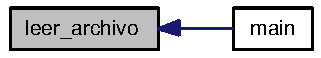
\includegraphics[width=95pt]{group__genetic_g6fed4910dd1f6172bb5a4e35a97bbe56_g6fed4910dd1f6172bb5a4e35a97bbe56_icgraph}
\end{center}
\end{figure}
\hypertarget{group__genetic_gc7ba874876f18abab66f0a42f32b98cc_gc7ba874876f18abab66f0a42f32b98cc}{
\index{genetic@{genetic}!population_create@{population\_\-create}}
\index{population_create@{population\_\-create}!genetic@{genetic}}
\subsubsection[population\_\-create]{\setlength{\rightskip}{0pt plus 5cm}void population\_\-create (\hyperlink{struct__population}{population} $\ast$ {\em p}, \hyperlink{struct__genesting}{genesting} $\ast$ {\em g}, int {\em n})}}
\label{group__genetic_gc7ba874876f18abab66f0a42f32b98cc_gc7ba874876f18abab66f0a42f32b98cc}


Esta funcion crea una poblacion inicial de soluciones.

\begin{Desc}
\item[Par\'{a}metros:]
\begin{description}
\item[\mbox{$\rightarrow$} {\em p}]Poblacion \item[\mbox{$\leftarrow$} {\em g}]Genesting \item[\mbox{$\leftarrow$} {\em n}]Numero de elementos de la poblacion \end{description}
\end{Desc}


Definici\'{o}n en la l\'{\i}nea 23 del archivo population.c.

\begin{Code}\begin{verbatim}23                                                           {
24     int i;
25     p->ambiente=g;
26     p->nindividuos=n;
27     p->individuos = (individuo*) malloc(sizeof(individuo)*p->nindividuos);
28 
29     for (i=0;i<p->nindividuos;i++){
30             individuo_create(p->ambiente,&(p->individuos[i]));
31     }
32 };
\end{verbatim}\end{Code}




Gr\'{a}fico de llamadas para esta funci\'{o}n:\begin{figure}[H]
\begin{center}
\leavevmode
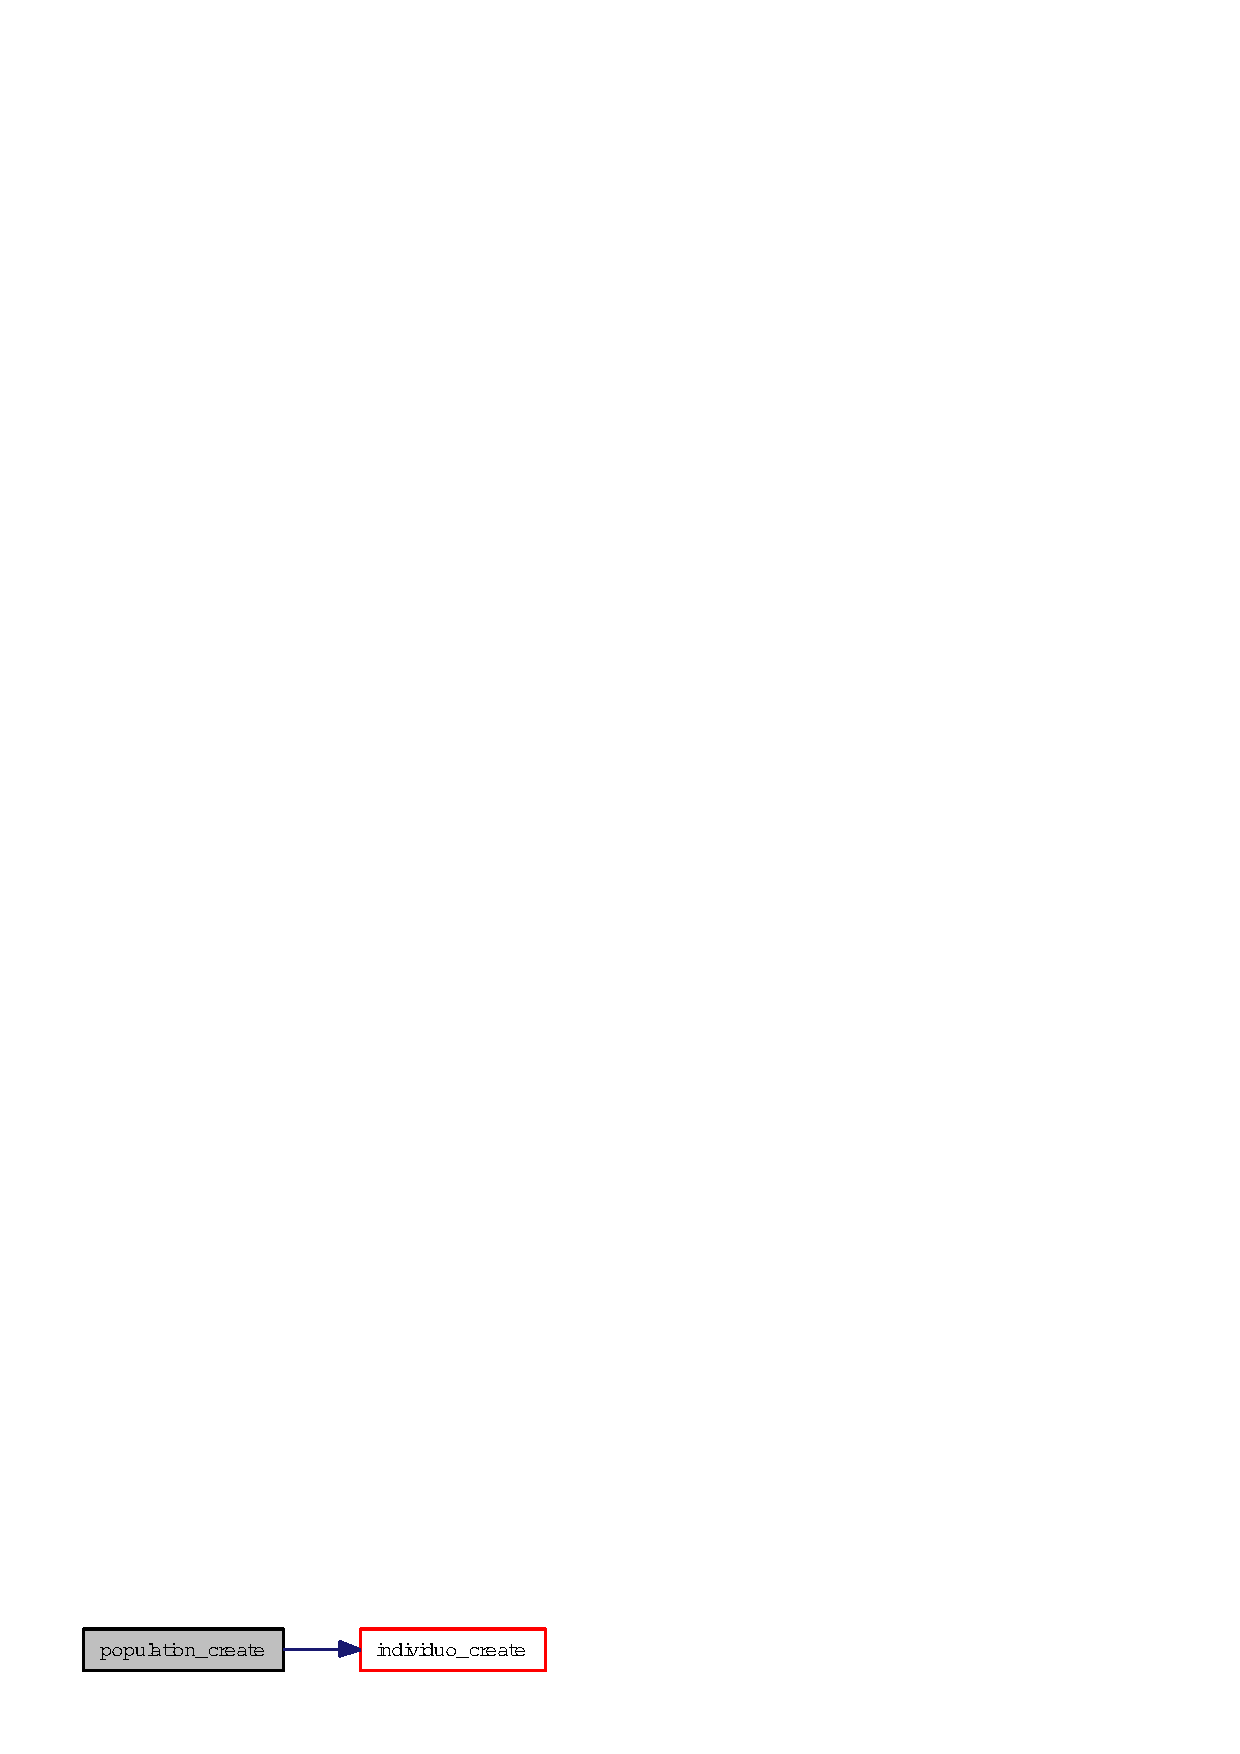
\includegraphics[width=133pt]{group__genetic_gc7ba874876f18abab66f0a42f32b98cc_gc7ba874876f18abab66f0a42f32b98cc_cgraph}
\end{center}
\end{figure}


Here is the caller graph for this function:\begin{figure}[H]
\begin{center}
\leavevmode
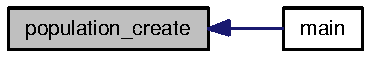
\includegraphics[width=107pt]{group__genetic_gc7ba874876f18abab66f0a42f32b98cc_gc7ba874876f18abab66f0a42f32b98cc_icgraph}
\end{center}
\end{figure}
\hypertarget{group__genetic_g229293c432c5ef4f70b1ee94c109bb1a_g229293c432c5ef4f70b1ee94c109bb1a}{
\index{genetic@{genetic}!population_evaluate@{population\_\-evaluate}}
\index{population_evaluate@{population\_\-evaluate}!genetic@{genetic}}
\subsubsection[population\_\-evaluate]{\setlength{\rightskip}{0pt plus 5cm}void population\_\-evaluate (\hyperlink{struct__population}{population} $\ast$ {\em p})}}
\label{group__genetic_g229293c432c5ef4f70b1ee94c109bb1a_g229293c432c5ef4f70b1ee94c109bb1a}


Evalua una poblacion, para esto calcula todos los fitness, y ordena los individuos segun su fitness

\begin{Desc}
\item[Par\'{a}metros:]
\begin{description}
\item[\mbox{$\leftrightarrow$} {\em p}]Poblacion \end{description}
\end{Desc}


Definici\'{o}n en la l\'{\i}nea 32 del archivo population.c.

Here is the caller graph for this function:\begin{figure}[H]
\begin{center}
\leavevmode
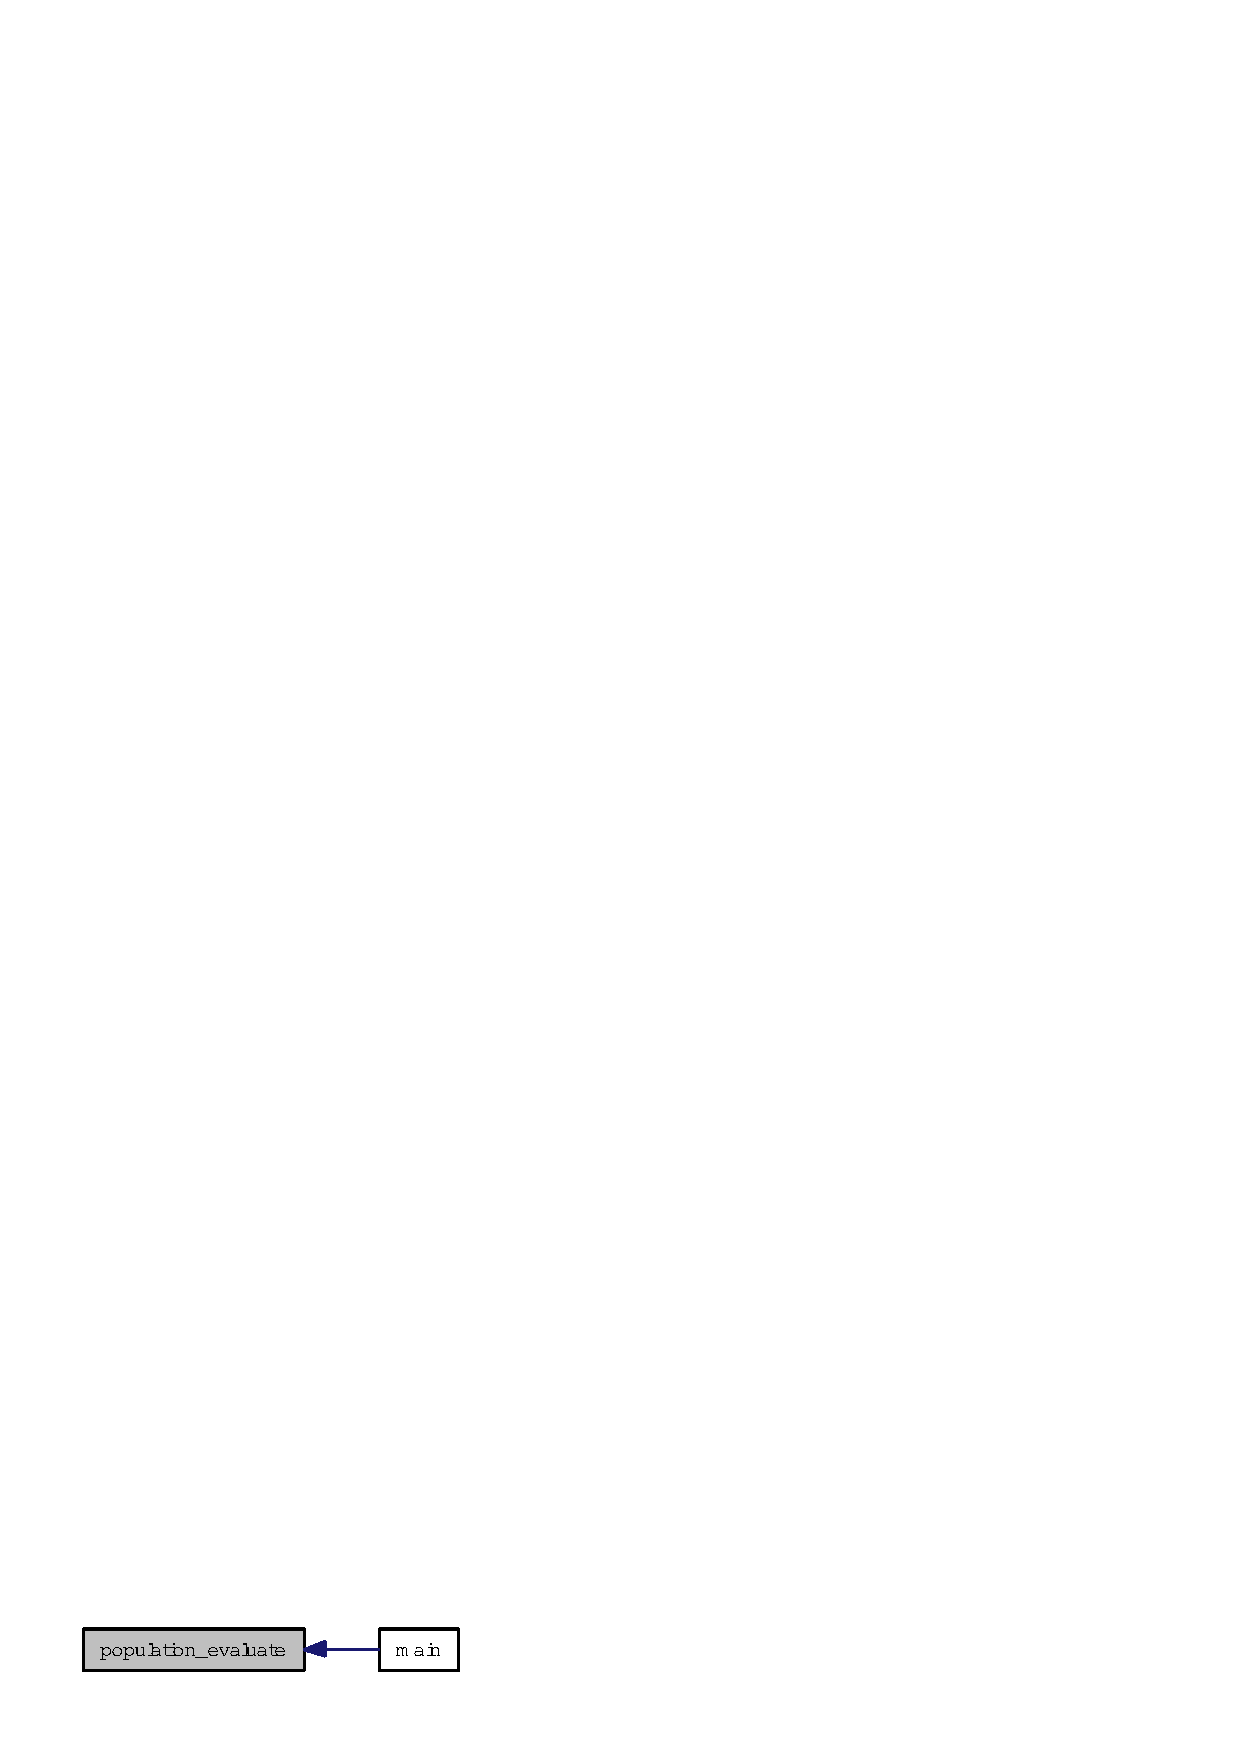
\includegraphics[width=112pt]{group__genetic_g229293c432c5ef4f70b1ee94c109bb1a_g229293c432c5ef4f70b1ee94c109bb1a_icgraph}
\end{center}
\end{figure}
\hypertarget{group__genetic_g5b3202f02e14d7fb3eb1f729d1250243_g5b3202f02e14d7fb3eb1f729d1250243}{
\index{genetic@{genetic}!population_generation@{population\_\-generation}}
\index{population_generation@{population\_\-generation}!genetic@{genetic}}
\subsubsection[population\_\-generation]{\setlength{\rightskip}{0pt plus 5cm}void population\_\-generation (\hyperlink{struct__population}{population} $\ast$ {\em p})}}
\label{group__genetic_g5b3202f02e14d7fb3eb1f729d1250243_g5b3202f02e14d7fb3eb1f729d1250243}


Crea una nueva poblacion, dividiendo la exitente en tres grupos, dejando el primer grupo intacto, el segundo lo muta, y el tercero es un cruce de los 2 primeros \begin{Desc}
\item[Par\'{a}metros:]
\begin{description}
\item[\mbox{$\leftrightarrow$} {\em p}]Poblacion \end{description}
\end{Desc}


Definici\'{o}n en la l\'{\i}nea 47 del archivo population.c.

Here is the caller graph for this function:\begin{figure}[H]
\begin{center}
\leavevmode
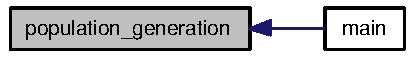
\includegraphics[width=117pt]{group__genetic_g5b3202f02e14d7fb3eb1f729d1250243_g5b3202f02e14d7fb3eb1f729d1250243_icgraph}
\end{center}
\end{figure}

\chapter{Genesting Documentaci\'{o}n de clases}
\hypertarget{struct__genesting}{
\section{Referencia de la Estructura \_\-genesting}
\label{struct__genesting}\index{_genesting@{\_\-genesting}}
}
{\tt \#include $<$genesting.h$>$}

Diagrama de colaboraci\'{o}n para \_\-genesting:\begin{figure}[H]
\begin{center}
\leavevmode
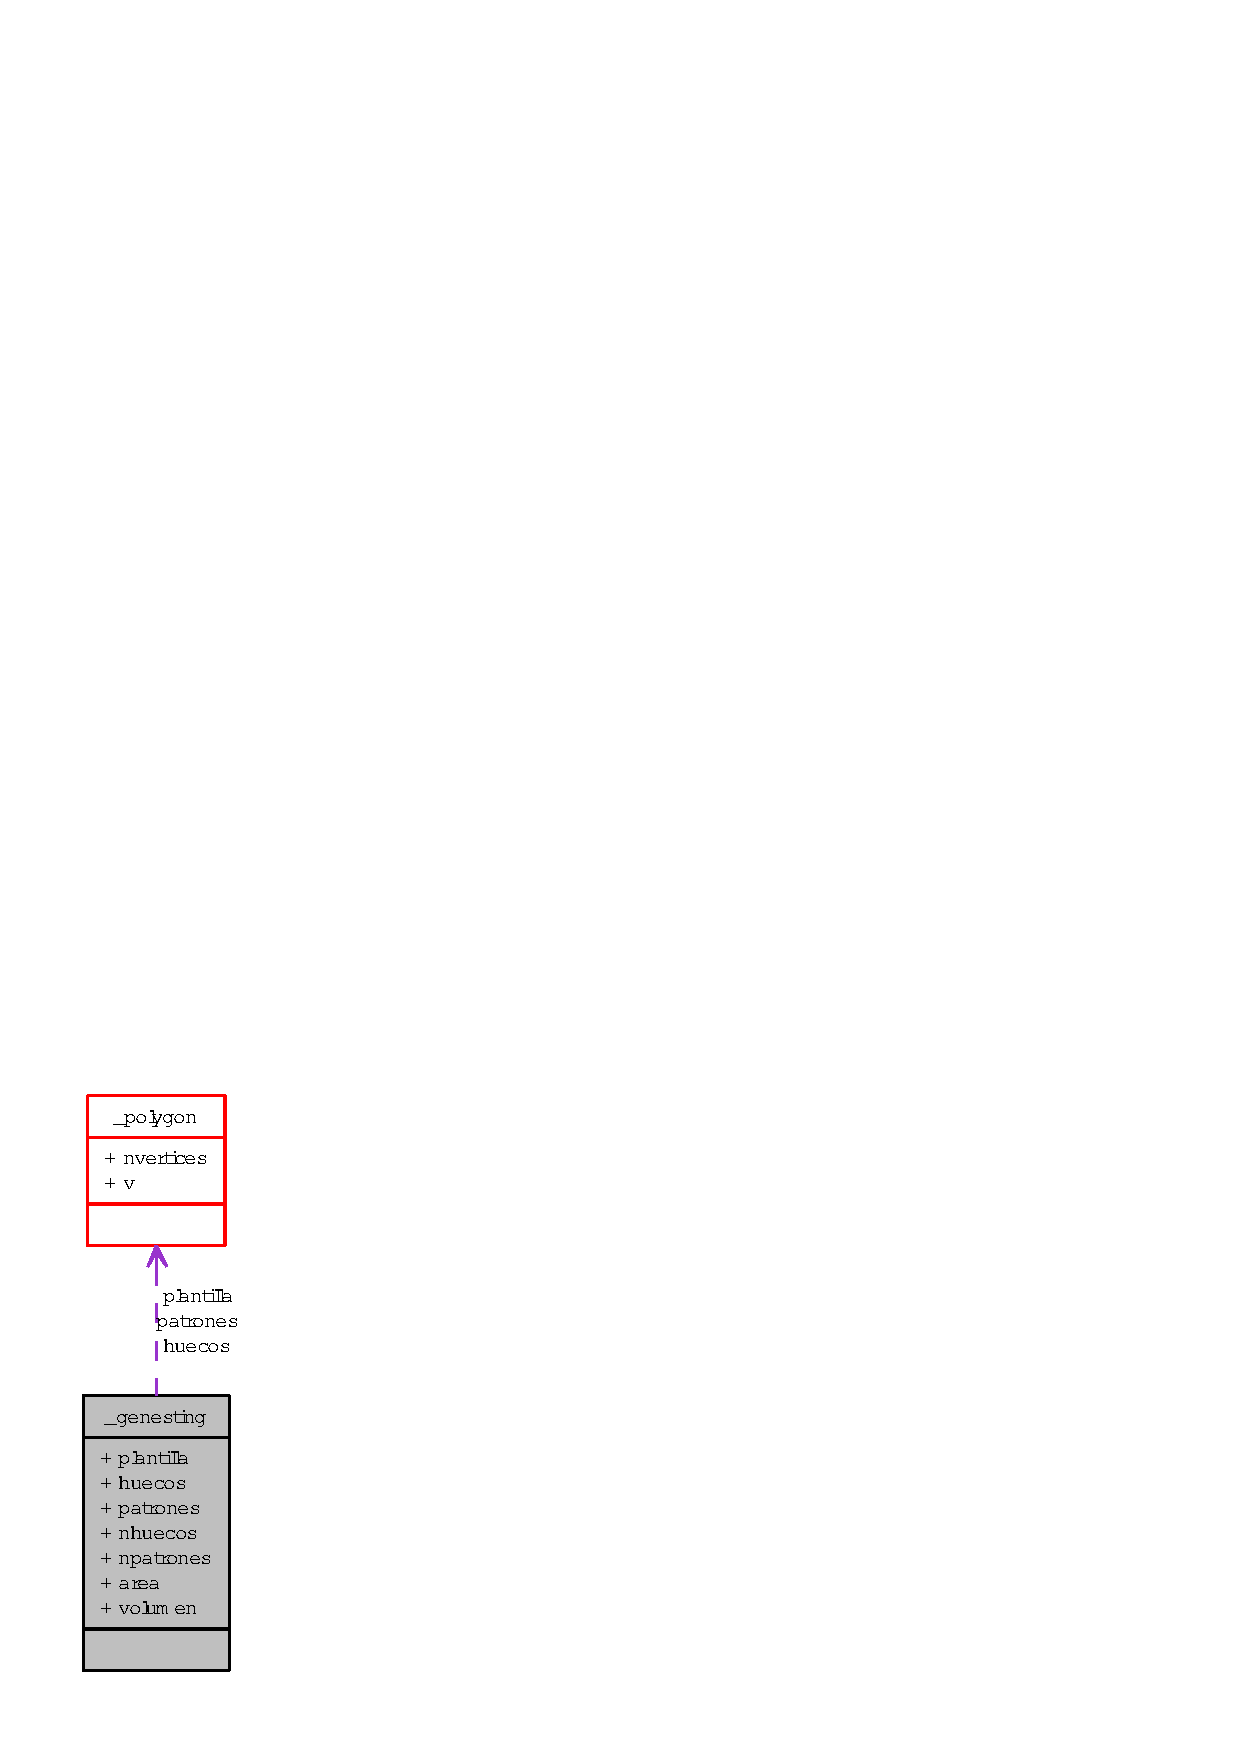
\includegraphics[width=59pt]{struct__genesting__coll__graph}
\end{center}
\end{figure}


\subsection{Descripci\'{o}n detallada}




Definici\'{o}n en la l\'{\i}nea 14 del archivo genesting.h.\subsection*{Atributos p\'{u}blicos}
\begin{CompactItemize}
\item 
\hyperlink{struct__polygon}{polygon} \hyperlink{struct__genesting_c660e2710da2db9469813d0a14981cef_c660e2710da2db9469813d0a14981cef}{plantilla}
\item 
\hyperlink{struct__polygon}{polygon} $\ast$ \hyperlink{struct__genesting_3affb28e2ad244f35baed248e3c230f6_3affb28e2ad244f35baed248e3c230f6}{huecos}
\item 
\hyperlink{struct__polygon}{polygon} $\ast$ \hyperlink{struct__genesting_c4b1743e42547577dbb6d7238ad4db17_c4b1743e42547577dbb6d7238ad4db17}{patrones}
\item 
unsigned int \hyperlink{struct__genesting_87ae802e5ffa06a1b38ce4337eadbcda_87ae802e5ffa06a1b38ce4337eadbcda}{nhuecos}
\item 
unsigned int \hyperlink{struct__genesting_a5ebd60476ce0253be4e5a09349433e1_a5ebd60476ce0253be4e5a09349433e1}{npatrones}
\item 
float \hyperlink{struct__genesting_052920321c80561169cd61a8eb301378_052920321c80561169cd61a8eb301378}{area}
\item 
float \hyperlink{struct__genesting_313b6909792763a5381ce7ff14830d6d_313b6909792763a5381ce7ff14830d6d}{volumen}
\end{CompactItemize}


\subsection{Documentaci\'{o}n de los datos miembro}
\hypertarget{struct__genesting_052920321c80561169cd61a8eb301378_052920321c80561169cd61a8eb301378}{
\index{_genesting@{\_\-genesting}!area@{area}}
\index{area@{area}!_genesting@{\_\-genesting}}
\subsubsection[area]{\setlength{\rightskip}{0pt plus 5cm}float \hyperlink{struct__genesting_052920321c80561169cd61a8eb301378_052920321c80561169cd61a8eb301378}{\_\-genesting::area}}}
\label{struct__genesting_052920321c80561169cd61a8eb301378_052920321c80561169cd61a8eb301378}




Definici\'{o}n en la l\'{\i}nea 21 del archivo genesting.h.\hypertarget{struct__genesting_3affb28e2ad244f35baed248e3c230f6_3affb28e2ad244f35baed248e3c230f6}{
\index{_genesting@{\_\-genesting}!huecos@{huecos}}
\index{huecos@{huecos}!_genesting@{\_\-genesting}}
\subsubsection[huecos]{\setlength{\rightskip}{0pt plus 5cm}\hyperlink{struct__polygon}{polygon}$\ast$ \hyperlink{struct__genesting_3affb28e2ad244f35baed248e3c230f6_3affb28e2ad244f35baed248e3c230f6}{\_\-genesting::huecos}}}
\label{struct__genesting_3affb28e2ad244f35baed248e3c230f6_3affb28e2ad244f35baed248e3c230f6}




Definici\'{o}n en la l\'{\i}nea 17 del archivo genesting.h.\hypertarget{struct__genesting_87ae802e5ffa06a1b38ce4337eadbcda_87ae802e5ffa06a1b38ce4337eadbcda}{
\index{_genesting@{\_\-genesting}!nhuecos@{nhuecos}}
\index{nhuecos@{nhuecos}!_genesting@{\_\-genesting}}
\subsubsection[nhuecos]{\setlength{\rightskip}{0pt plus 5cm}unsigned int \hyperlink{struct__genesting_87ae802e5ffa06a1b38ce4337eadbcda_87ae802e5ffa06a1b38ce4337eadbcda}{\_\-genesting::nhuecos}}}
\label{struct__genesting_87ae802e5ffa06a1b38ce4337eadbcda_87ae802e5ffa06a1b38ce4337eadbcda}




Definici\'{o}n en la l\'{\i}nea 19 del archivo genesting.h.\hypertarget{struct__genesting_a5ebd60476ce0253be4e5a09349433e1_a5ebd60476ce0253be4e5a09349433e1}{
\index{_genesting@{\_\-genesting}!npatrones@{npatrones}}
\index{npatrones@{npatrones}!_genesting@{\_\-genesting}}
\subsubsection[npatrones]{\setlength{\rightskip}{0pt plus 5cm}unsigned int \hyperlink{struct__genesting_a5ebd60476ce0253be4e5a09349433e1_a5ebd60476ce0253be4e5a09349433e1}{\_\-genesting::npatrones}}}
\label{struct__genesting_a5ebd60476ce0253be4e5a09349433e1_a5ebd60476ce0253be4e5a09349433e1}




Definici\'{o}n en la l\'{\i}nea 20 del archivo genesting.h.\hypertarget{struct__genesting_c4b1743e42547577dbb6d7238ad4db17_c4b1743e42547577dbb6d7238ad4db17}{
\index{_genesting@{\_\-genesting}!patrones@{patrones}}
\index{patrones@{patrones}!_genesting@{\_\-genesting}}
\subsubsection[patrones]{\setlength{\rightskip}{0pt plus 5cm}\hyperlink{struct__polygon}{polygon}$\ast$ \hyperlink{struct__genesting_c4b1743e42547577dbb6d7238ad4db17_c4b1743e42547577dbb6d7238ad4db17}{\_\-genesting::patrones}}}
\label{struct__genesting_c4b1743e42547577dbb6d7238ad4db17_c4b1743e42547577dbb6d7238ad4db17}




Definici\'{o}n en la l\'{\i}nea 18 del archivo genesting.h.\hypertarget{struct__genesting_c660e2710da2db9469813d0a14981cef_c660e2710da2db9469813d0a14981cef}{
\index{_genesting@{\_\-genesting}!plantilla@{plantilla}}
\index{plantilla@{plantilla}!_genesting@{\_\-genesting}}
\subsubsection[plantilla]{\setlength{\rightskip}{0pt plus 5cm}\hyperlink{struct__polygon}{polygon} \hyperlink{struct__genesting_c660e2710da2db9469813d0a14981cef_c660e2710da2db9469813d0a14981cef}{\_\-genesting::plantilla}}}
\label{struct__genesting_c660e2710da2db9469813d0a14981cef_c660e2710da2db9469813d0a14981cef}




Definici\'{o}n en la l\'{\i}nea 16 del archivo genesting.h.\hypertarget{struct__genesting_313b6909792763a5381ce7ff14830d6d_313b6909792763a5381ce7ff14830d6d}{
\index{_genesting@{\_\-genesting}!volumen@{volumen}}
\index{volumen@{volumen}!_genesting@{\_\-genesting}}
\subsubsection[volumen]{\setlength{\rightskip}{0pt plus 5cm}float \hyperlink{struct__genesting_313b6909792763a5381ce7ff14830d6d_313b6909792763a5381ce7ff14830d6d}{\_\-genesting::volumen}}}
\label{struct__genesting_313b6909792763a5381ce7ff14830d6d_313b6909792763a5381ce7ff14830d6d}




Definici\'{o}n en la l\'{\i}nea 22 del archivo genesting.h.

La documentaci\'{o}n para esta estructura fu\'{e} generada a partir del siguiente archivo:\begin{CompactItemize}
\item 
\hyperlink{genesting_8h}{genesting.h}\end{CompactItemize}

\hypertarget{struct__individuo}{
\section{Referencia de la Estructura \_\-individuo}
\label{struct__individuo}\index{_individuo@{\_\-individuo}}
}
{\tt \#include $<$individuo.h$>$}

Diagrama de colaboraci\'{o}n para \_\-individuo:\begin{figure}[H]
\begin{center}
\leavevmode
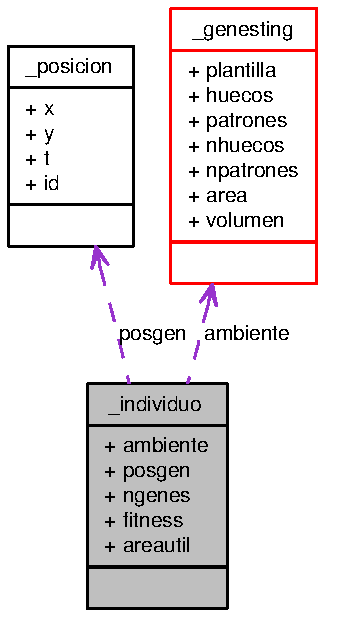
\includegraphics[width=99pt]{struct__individuo__coll__graph}
\end{center}
\end{figure}


\subsection{Descripci\'{o}n detallada}




Definici\'{o}n en la l\'{\i}nea 29 del archivo individuo.h.\subsection*{Atributos p\'{u}blicos}
\begin{CompactItemize}
\item 
\hyperlink{struct__genesting}{genesting} $\ast$ \hyperlink{struct__individuo_77db4f35b317761eeb9a0cb2b8f8276d_77db4f35b317761eeb9a0cb2b8f8276d}{ambiente}
\item 
\hyperlink{struct__posicion}{posicion} $\ast$ \hyperlink{struct__individuo_2187e821ff69e7e3de9fa511745f976a_2187e821ff69e7e3de9fa511745f976a}{posgen}
\item 
unsigned int \hyperlink{struct__individuo_6ca41cfab8bba8bd7c2ba8f44d2407f1_6ca41cfab8bba8bd7c2ba8f44d2407f1}{ngenes}
\item 
float \hyperlink{struct__individuo_afa717374da03fa5ef2c5ac8c08e1daa_afa717374da03fa5ef2c5ac8c08e1daa}{fitness}
\item 
float \hyperlink{struct__individuo_81afc3d6d6f5394611dcd09a418ee828_81afc3d6d6f5394611dcd09a418ee828}{areautil}
\end{CompactItemize}


\subsection{Documentaci\'{o}n de los datos miembro}
\hypertarget{struct__individuo_77db4f35b317761eeb9a0cb2b8f8276d_77db4f35b317761eeb9a0cb2b8f8276d}{
\index{_individuo@{\_\-individuo}!ambiente@{ambiente}}
\index{ambiente@{ambiente}!_individuo@{\_\-individuo}}
\subsubsection[ambiente]{\setlength{\rightskip}{0pt plus 5cm}\hyperlink{struct__genesting}{genesting}$\ast$ \hyperlink{struct__individuo_77db4f35b317761eeb9a0cb2b8f8276d_77db4f35b317761eeb9a0cb2b8f8276d}{\_\-individuo::ambiente}}}
\label{struct__individuo_77db4f35b317761eeb9a0cb2b8f8276d_77db4f35b317761eeb9a0cb2b8f8276d}




Definici\'{o}n en la l\'{\i}nea 31 del archivo individuo.h.\hypertarget{struct__individuo_81afc3d6d6f5394611dcd09a418ee828_81afc3d6d6f5394611dcd09a418ee828}{
\index{_individuo@{\_\-individuo}!areautil@{areautil}}
\index{areautil@{areautil}!_individuo@{\_\-individuo}}
\subsubsection[areautil]{\setlength{\rightskip}{0pt plus 5cm}float \hyperlink{struct__individuo_81afc3d6d6f5394611dcd09a418ee828_81afc3d6d6f5394611dcd09a418ee828}{\_\-individuo::areautil}}}
\label{struct__individuo_81afc3d6d6f5394611dcd09a418ee828_81afc3d6d6f5394611dcd09a418ee828}




Definici\'{o}n en la l\'{\i}nea 36 del archivo individuo.h.\hypertarget{struct__individuo_afa717374da03fa5ef2c5ac8c08e1daa_afa717374da03fa5ef2c5ac8c08e1daa}{
\index{_individuo@{\_\-individuo}!fitness@{fitness}}
\index{fitness@{fitness}!_individuo@{\_\-individuo}}
\subsubsection[fitness]{\setlength{\rightskip}{0pt plus 5cm}float \hyperlink{struct__individuo_afa717374da03fa5ef2c5ac8c08e1daa_afa717374da03fa5ef2c5ac8c08e1daa}{\_\-individuo::fitness}}}
\label{struct__individuo_afa717374da03fa5ef2c5ac8c08e1daa_afa717374da03fa5ef2c5ac8c08e1daa}




Definici\'{o}n en la l\'{\i}nea 35 del archivo individuo.h.\hypertarget{struct__individuo_6ca41cfab8bba8bd7c2ba8f44d2407f1_6ca41cfab8bba8bd7c2ba8f44d2407f1}{
\index{_individuo@{\_\-individuo}!ngenes@{ngenes}}
\index{ngenes@{ngenes}!_individuo@{\_\-individuo}}
\subsubsection[ngenes]{\setlength{\rightskip}{0pt plus 5cm}unsigned int \hyperlink{struct__individuo_6ca41cfab8bba8bd7c2ba8f44d2407f1_6ca41cfab8bba8bd7c2ba8f44d2407f1}{\_\-individuo::ngenes}}}
\label{struct__individuo_6ca41cfab8bba8bd7c2ba8f44d2407f1_6ca41cfab8bba8bd7c2ba8f44d2407f1}




Definici\'{o}n en la l\'{\i}nea 34 del archivo individuo.h.\hypertarget{struct__individuo_2187e821ff69e7e3de9fa511745f976a_2187e821ff69e7e3de9fa511745f976a}{
\index{_individuo@{\_\-individuo}!posgen@{posgen}}
\index{posgen@{posgen}!_individuo@{\_\-individuo}}
\subsubsection[posgen]{\setlength{\rightskip}{0pt plus 5cm}\hyperlink{struct__posicion}{posicion}$\ast$ \hyperlink{struct__individuo_2187e821ff69e7e3de9fa511745f976a_2187e821ff69e7e3de9fa511745f976a}{\_\-individuo::posgen}}}
\label{struct__individuo_2187e821ff69e7e3de9fa511745f976a_2187e821ff69e7e3de9fa511745f976a}




Definici\'{o}n en la l\'{\i}nea 32 del archivo individuo.h.

La documentaci\'{o}n para esta estructura fu\'{e} generada a partir del siguiente archivo:\begin{CompactItemize}
\item 
\hyperlink{individuo_8h}{individuo.h}\end{CompactItemize}

\hypertarget{struct__line}{
\section{Referencia de la Estructura \_\-line}
\label{struct__line}\index{_line@{\_\-line}}
}
{\tt \#include $<$line.h$>$}

Diagrama de colaboraci\'{o}n para \_\-line:\begin{figure}[H]
\begin{center}
\leavevmode
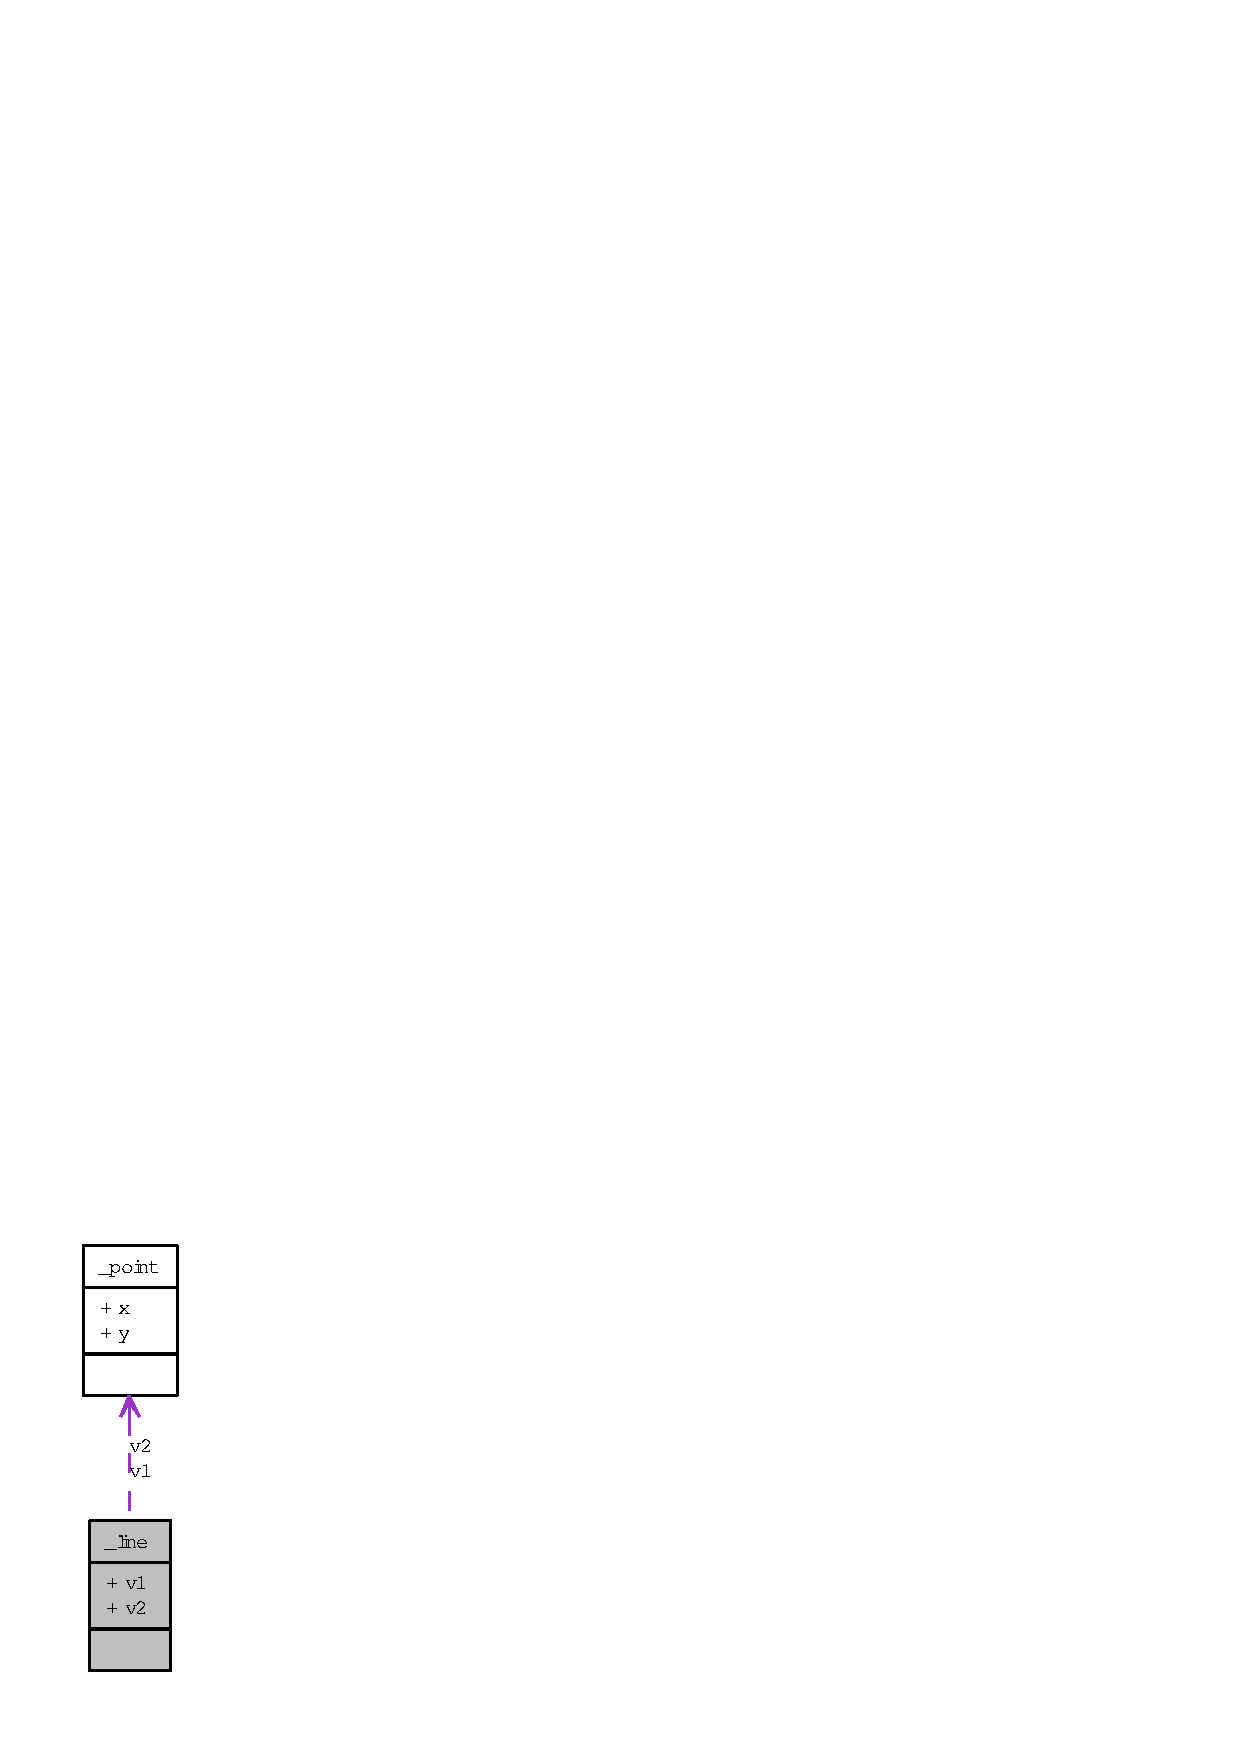
\includegraphics[width=44pt]{struct__line__coll__graph}
\end{center}
\end{figure}


\subsection{Descripci\'{o}n detallada}




Definici\'{o}n en la l\'{\i}nea 16 del archivo line.h.\subsection*{Atributos p\'{u}blicos}
\begin{CompactItemize}
\item 
\hyperlink{struct__point}{point} \hyperlink{struct__line_b70e9dced9e0d20c06fa5bdbb1e7be2d_b70e9dced9e0d20c06fa5bdbb1e7be2d}{v1}
\item 
\hyperlink{struct__point}{point} \hyperlink{struct__line_5701d84b34e7ca18c5a246d8f18239c2_5701d84b34e7ca18c5a246d8f18239c2}{v2}
\end{CompactItemize}


\subsection{Documentaci\'{o}n de los datos miembro}
\hypertarget{struct__line_b70e9dced9e0d20c06fa5bdbb1e7be2d_b70e9dced9e0d20c06fa5bdbb1e7be2d}{
\index{_line@{\_\-line}!v1@{v1}}
\index{v1@{v1}!_line@{\_\-line}}
\subsubsection[v1]{\setlength{\rightskip}{0pt plus 5cm}\hyperlink{struct__point}{point} \hyperlink{struct__line_b70e9dced9e0d20c06fa5bdbb1e7be2d_b70e9dced9e0d20c06fa5bdbb1e7be2d}{\_\-line::v1}}}
\label{struct__line_b70e9dced9e0d20c06fa5bdbb1e7be2d_b70e9dced9e0d20c06fa5bdbb1e7be2d}




Definici\'{o}n en la l\'{\i}nea 18 del archivo line.h.\hypertarget{struct__line_5701d84b34e7ca18c5a246d8f18239c2_5701d84b34e7ca18c5a246d8f18239c2}{
\index{_line@{\_\-line}!v2@{v2}}
\index{v2@{v2}!_line@{\_\-line}}
\subsubsection[v2]{\setlength{\rightskip}{0pt plus 5cm}\hyperlink{struct__point}{point} \hyperlink{struct__line_5701d84b34e7ca18c5a246d8f18239c2_5701d84b34e7ca18c5a246d8f18239c2}{\_\-line::v2}}}
\label{struct__line_5701d84b34e7ca18c5a246d8f18239c2_5701d84b34e7ca18c5a246d8f18239c2}




Definici\'{o}n en la l\'{\i}nea 18 del archivo line.h.

La documentaci\'{o}n para esta estructura fu\'{e} generada a partir del siguiente archivo:\begin{CompactItemize}
\item 
\hyperlink{line_8h}{line.h}\end{CompactItemize}

\hypertarget{struct__point}{
\section{Referencia de la Estructura \_\-point}
\label{struct__point}\index{_point@{\_\-point}}
}
{\tt \#include $<$point.h$>$}



\subsection{Descripci\'{o}n detallada}




Definici\'{o}n en la l\'{\i}nea 12 del archivo point.h.\subsection*{Atributos p\'{u}blicos}
\begin{CompactItemize}
\item 
float \hyperlink{struct__point_767ac72154b321228732c3dad513eb27_767ac72154b321228732c3dad513eb27}{x}
\item 
float \hyperlink{struct__point_8959fb193a9a1f2cb450a79d3dfc5b0e_8959fb193a9a1f2cb450a79d3dfc5b0e}{y}
\end{CompactItemize}


\subsection{Documentaci\'{o}n de los datos miembro}
\hypertarget{struct__point_767ac72154b321228732c3dad513eb27_767ac72154b321228732c3dad513eb27}{
\index{_point@{\_\-point}!x@{x}}
\index{x@{x}!_point@{\_\-point}}
\subsubsection[x]{\setlength{\rightskip}{0pt plus 5cm}float \hyperlink{struct__point_767ac72154b321228732c3dad513eb27_767ac72154b321228732c3dad513eb27}{\_\-point::x}}}
\label{struct__point_767ac72154b321228732c3dad513eb27_767ac72154b321228732c3dad513eb27}




Definici\'{o}n en la l\'{\i}nea 14 del archivo point.h.\hypertarget{struct__point_8959fb193a9a1f2cb450a79d3dfc5b0e_8959fb193a9a1f2cb450a79d3dfc5b0e}{
\index{_point@{\_\-point}!y@{y}}
\index{y@{y}!_point@{\_\-point}}
\subsubsection[y]{\setlength{\rightskip}{0pt plus 5cm}float \hyperlink{struct__point_8959fb193a9a1f2cb450a79d3dfc5b0e_8959fb193a9a1f2cb450a79d3dfc5b0e}{\_\-point::y}}}
\label{struct__point_8959fb193a9a1f2cb450a79d3dfc5b0e_8959fb193a9a1f2cb450a79d3dfc5b0e}




Definici\'{o}n en la l\'{\i}nea 15 del archivo point.h.

La documentaci\'{o}n para esta estructura fu\'{e} generada a partir del siguiente archivo:\begin{CompactItemize}
\item 
\hyperlink{point_8h}{point.h}\end{CompactItemize}

\hypertarget{struct__polygon}{
\section{Referencia de la Estructura \_\-polygon}
\label{struct__polygon}\index{_polygon@{\_\-polygon}}
}
{\tt \#include $<$polygon.h$>$}

Diagrama de colaboraci\'{o}n para \_\-polygon:\begin{figure}[H]
\begin{center}
\leavevmode
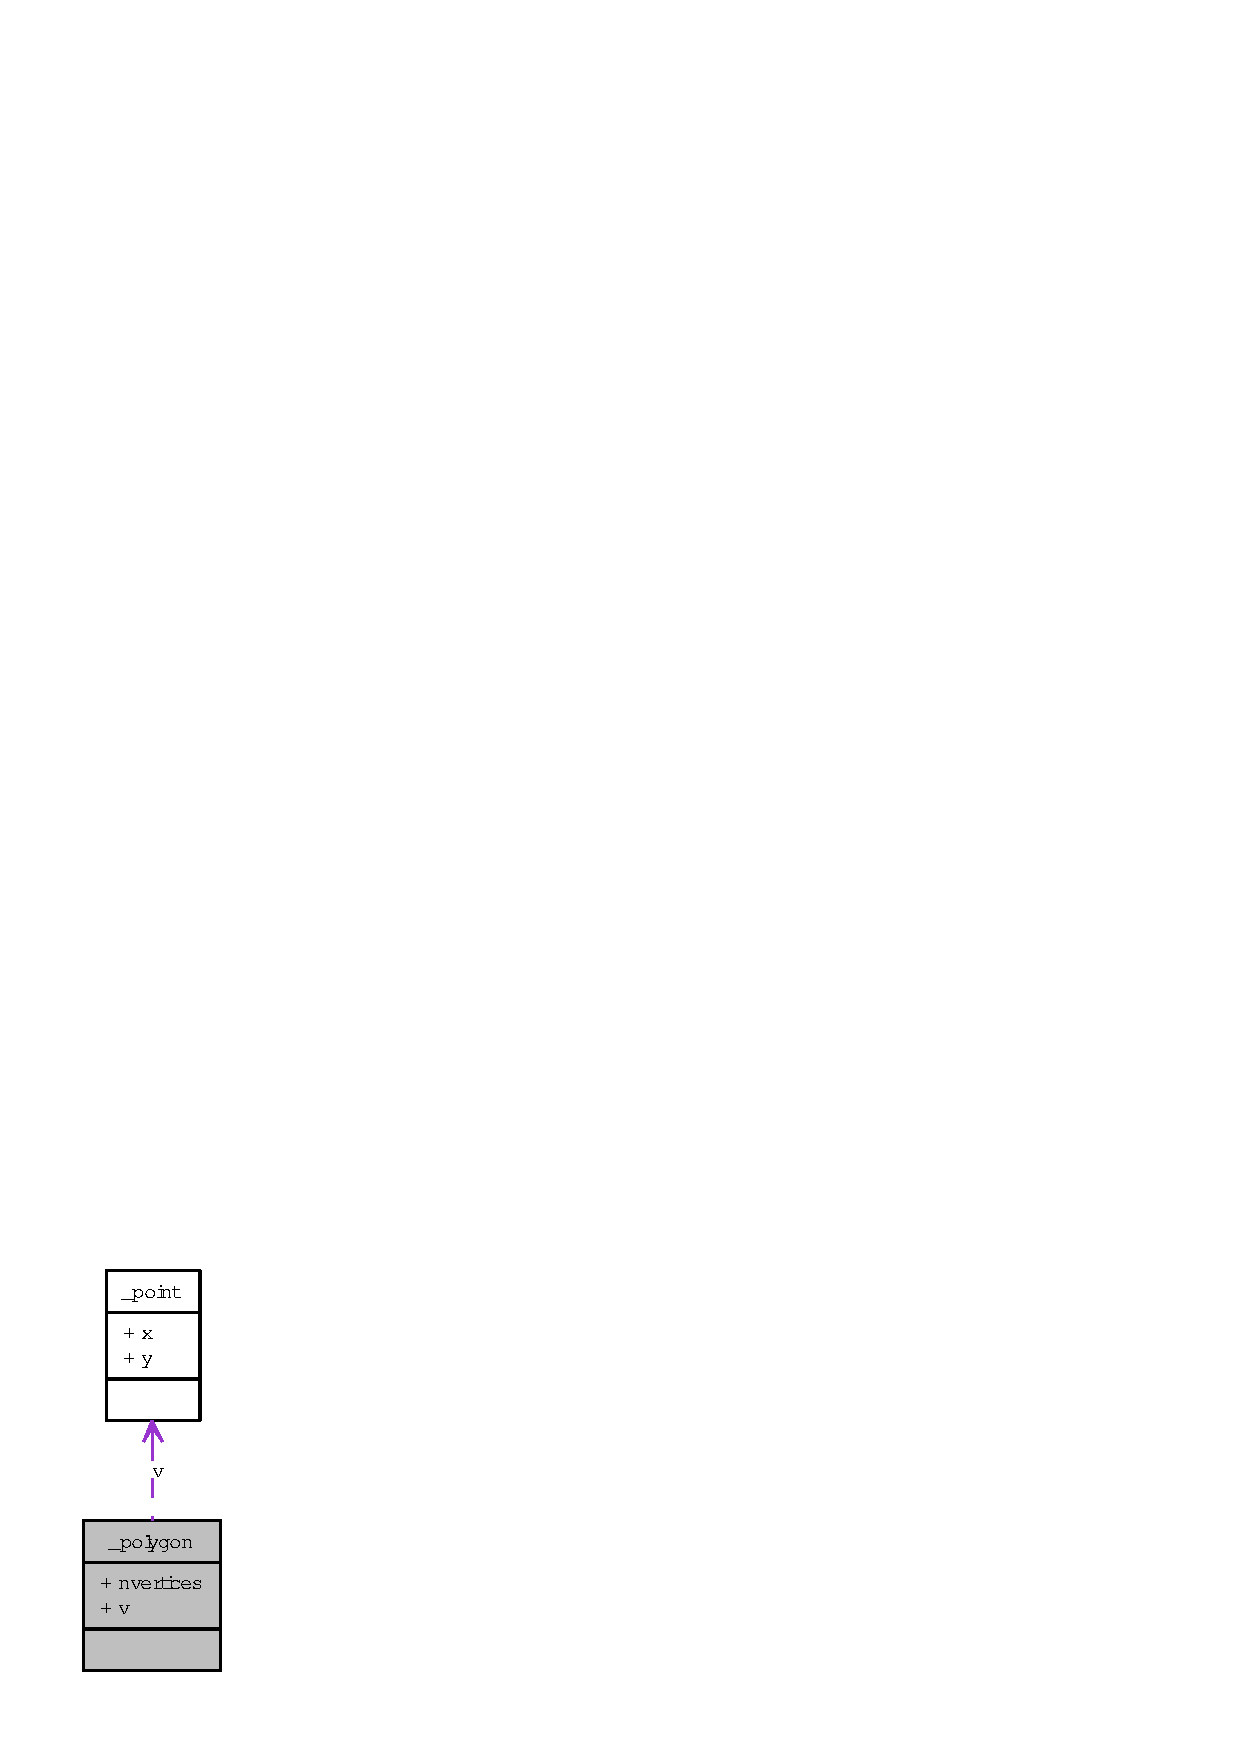
\includegraphics[width=55pt]{struct__polygon__coll__graph}
\end{center}
\end{figure}


\subsection{Descripci\'{o}n detallada}




Definici\'{o}n en la l\'{\i}nea 18 del archivo polygon.h.\subsection*{Atributos p\'{u}blicos}
\begin{CompactItemize}
\item 
unsigned int \hyperlink{struct__polygon_32b823ec27d32ee03ab132c173d3672a_32b823ec27d32ee03ab132c173d3672a}{nvertices}
\item 
\hyperlink{struct__point}{point} $\ast$ \hyperlink{struct__polygon_32ccf29956c65625eddb9f4c75ce0f0c_32ccf29956c65625eddb9f4c75ce0f0c}{v}
\end{CompactItemize}


\subsection{Documentaci\'{o}n de los datos miembro}
\hypertarget{struct__polygon_32b823ec27d32ee03ab132c173d3672a_32b823ec27d32ee03ab132c173d3672a}{
\index{_polygon@{\_\-polygon}!nvertices@{nvertices}}
\index{nvertices@{nvertices}!_polygon@{\_\-polygon}}
\subsubsection[nvertices]{\setlength{\rightskip}{0pt plus 5cm}unsigned int \hyperlink{struct__polygon_32b823ec27d32ee03ab132c173d3672a_32b823ec27d32ee03ab132c173d3672a}{\_\-polygon::nvertices}}}
\label{struct__polygon_32b823ec27d32ee03ab132c173d3672a_32b823ec27d32ee03ab132c173d3672a}




Definici\'{o}n en la l\'{\i}nea 20 del archivo polygon.h.\hypertarget{struct__polygon_32ccf29956c65625eddb9f4c75ce0f0c_32ccf29956c65625eddb9f4c75ce0f0c}{
\index{_polygon@{\_\-polygon}!v@{v}}
\index{v@{v}!_polygon@{\_\-polygon}}
\subsubsection[v]{\setlength{\rightskip}{0pt plus 5cm}\hyperlink{struct__point}{point}$\ast$ \hyperlink{struct__polygon_32ccf29956c65625eddb9f4c75ce0f0c_32ccf29956c65625eddb9f4c75ce0f0c}{\_\-polygon::v}}}
\label{struct__polygon_32ccf29956c65625eddb9f4c75ce0f0c_32ccf29956c65625eddb9f4c75ce0f0c}




Definici\'{o}n en la l\'{\i}nea 21 del archivo polygon.h.

La documentaci\'{o}n para esta estructura fu\'{e} generada a partir del siguiente archivo:\begin{CompactItemize}
\item 
\hyperlink{polygon_8h}{polygon.h}\end{CompactItemize}

\hypertarget{struct__polygon__holes}{
\section{Referencia de la Estructura \_\-polygon\_\-holes}
\label{struct__polygon__holes}\index{_polygon_holes@{\_\-polygon\_\-holes}}
}
{\tt \#include $<$polygon\_\-holes.h$>$}

Diagrama de colaboraci\'{o}n para \_\-polygon\_\-holes:\begin{figure}[H]
\begin{center}
\leavevmode
\includegraphics[width=65pt]{struct__polygon__holes__coll__graph}
\end{center}
\end{figure}


\subsection{Descripci\'{o}n detallada}




Definici\'{o}n en la l\'{\i}nea 17 del archivo polygon\_\-holes.h.\subsection*{Atributos p\'{u}blicos}
\begin{CompactItemize}
\item 
unsigned int \hyperlink{struct__polygon__holes_dc7994045ce07712cf57b791ccaa0015_dc7994045ce07712cf57b791ccaa0015}{nholes}
\item 
\hyperlink{struct__polygon}{polygon} $\ast$ \hyperlink{struct__polygon__holes_90635c34b3613c8cf8cdda5bebe99638_90635c34b3613c8cf8cdda5bebe99638}{p}
\item 
\hyperlink{struct__polygon}{polygon} $\ast$ \hyperlink{struct__polygon__holes_b2a2b78ef53f56d9f4a7639c9dd15fd0_b2a2b78ef53f56d9f4a7639c9dd15fd0}{h}
\end{CompactItemize}


\subsection{Documentaci\'{o}n de los datos miembro}
\hypertarget{struct__polygon__holes_b2a2b78ef53f56d9f4a7639c9dd15fd0_b2a2b78ef53f56d9f4a7639c9dd15fd0}{
\index{_polygon_holes@{\_\-polygon\_\-holes}!h@{h}}
\index{h@{h}!_polygon_holes@{\_\-polygon\_\-holes}}
\subsubsection[h]{\setlength{\rightskip}{0pt plus 5cm}\hyperlink{struct__polygon}{polygon}$\ast$ \hyperlink{struct__polygon__holes_b2a2b78ef53f56d9f4a7639c9dd15fd0_b2a2b78ef53f56d9f4a7639c9dd15fd0}{\_\-polygon\_\-holes::h}}}
\label{struct__polygon__holes_b2a2b78ef53f56d9f4a7639c9dd15fd0_b2a2b78ef53f56d9f4a7639c9dd15fd0}




Definici\'{o}n en la l\'{\i}nea 21 del archivo polygon\_\-holes.h.\hypertarget{struct__polygon__holes_dc7994045ce07712cf57b791ccaa0015_dc7994045ce07712cf57b791ccaa0015}{
\index{_polygon_holes@{\_\-polygon\_\-holes}!nholes@{nholes}}
\index{nholes@{nholes}!_polygon_holes@{\_\-polygon\_\-holes}}
\subsubsection[nholes]{\setlength{\rightskip}{0pt plus 5cm}unsigned int \hyperlink{struct__polygon__holes_dc7994045ce07712cf57b791ccaa0015_dc7994045ce07712cf57b791ccaa0015}{\_\-polygon\_\-holes::nholes}}}
\label{struct__polygon__holes_dc7994045ce07712cf57b791ccaa0015_dc7994045ce07712cf57b791ccaa0015}




Definici\'{o}n en la l\'{\i}nea 19 del archivo polygon\_\-holes.h.\hypertarget{struct__polygon__holes_90635c34b3613c8cf8cdda5bebe99638_90635c34b3613c8cf8cdda5bebe99638}{
\index{_polygon_holes@{\_\-polygon\_\-holes}!p@{p}}
\index{p@{p}!_polygon_holes@{\_\-polygon\_\-holes}}
\subsubsection[p]{\setlength{\rightskip}{0pt plus 5cm}\hyperlink{struct__polygon}{polygon}$\ast$ \hyperlink{struct__polygon__holes_90635c34b3613c8cf8cdda5bebe99638_90635c34b3613c8cf8cdda5bebe99638}{\_\-polygon\_\-holes::p}}}
\label{struct__polygon__holes_90635c34b3613c8cf8cdda5bebe99638_90635c34b3613c8cf8cdda5bebe99638}




Definici\'{o}n en la l\'{\i}nea 20 del archivo polygon\_\-holes.h.

La documentaci\'{o}n para esta estructura fu\'{e} generada a partir del siguiente archivo:\begin{CompactItemize}
\item 
\hyperlink{polygon__holes_8h}{polygon\_\-holes.h}\end{CompactItemize}

\hypertarget{struct__population}{
\section{Referencia de la Estructura \_\-population}
\label{struct__population}\index{_population@{\_\-population}}
}
{\tt \#include $<$population.h$>$}

Diagrama de colaboraci\'{o}n para \_\-population:\begin{figure}[H]
\begin{center}
\leavevmode
\includegraphics[width=94pt]{struct__population__coll__graph}
\end{center}
\end{figure}


\subsection{Descripci\'{o}n detallada}




Definici\'{o}n en la l\'{\i}nea 15 del archivo population.h.\subsection*{Atributos p\'{u}blicos}
\begin{CompactItemize}
\item 
\hyperlink{struct__genesting}{genesting} $\ast$ \hyperlink{struct__population_68ccc9819f5face92f988074d5b1a8af_68ccc9819f5face92f988074d5b1a8af}{ambiente}
\item 
int \hyperlink{struct__population_6dc56f2e17990f5e0ae27324e27f948e_6dc56f2e17990f5e0ae27324e27f948e}{nindividuos}
\item 
\hyperlink{struct__individuo}{individuo} $\ast$ \hyperlink{struct__population_3c05b6054f79c3c7993559e3148752a9_3c05b6054f79c3c7993559e3148752a9}{individuos}
\end{CompactItemize}


\subsection{Documentaci\'{o}n de los datos miembro}
\hypertarget{struct__population_68ccc9819f5face92f988074d5b1a8af_68ccc9819f5face92f988074d5b1a8af}{
\index{_population@{\_\-population}!ambiente@{ambiente}}
\index{ambiente@{ambiente}!_population@{\_\-population}}
\subsubsection[ambiente]{\setlength{\rightskip}{0pt plus 5cm}\hyperlink{struct__genesting}{genesting}$\ast$ \hyperlink{struct__population_68ccc9819f5face92f988074d5b1a8af_68ccc9819f5face92f988074d5b1a8af}{\_\-population::ambiente}}}
\label{struct__population_68ccc9819f5face92f988074d5b1a8af_68ccc9819f5face92f988074d5b1a8af}




Definici\'{o}n en la l\'{\i}nea 16 del archivo population.h.\hypertarget{struct__population_3c05b6054f79c3c7993559e3148752a9_3c05b6054f79c3c7993559e3148752a9}{
\index{_population@{\_\-population}!individuos@{individuos}}
\index{individuos@{individuos}!_population@{\_\-population}}
\subsubsection[individuos]{\setlength{\rightskip}{0pt plus 5cm}\hyperlink{struct__individuo}{individuo}$\ast$ \hyperlink{struct__population_3c05b6054f79c3c7993559e3148752a9_3c05b6054f79c3c7993559e3148752a9}{\_\-population::individuos}}}
\label{struct__population_3c05b6054f79c3c7993559e3148752a9_3c05b6054f79c3c7993559e3148752a9}




Definici\'{o}n en la l\'{\i}nea 18 del archivo population.h.\hypertarget{struct__population_6dc56f2e17990f5e0ae27324e27f948e_6dc56f2e17990f5e0ae27324e27f948e}{
\index{_population@{\_\-population}!nindividuos@{nindividuos}}
\index{nindividuos@{nindividuos}!_population@{\_\-population}}
\subsubsection[nindividuos]{\setlength{\rightskip}{0pt plus 5cm}int \hyperlink{struct__population_6dc56f2e17990f5e0ae27324e27f948e_6dc56f2e17990f5e0ae27324e27f948e}{\_\-population::nindividuos}}}
\label{struct__population_6dc56f2e17990f5e0ae27324e27f948e_6dc56f2e17990f5e0ae27324e27f948e}




Definici\'{o}n en la l\'{\i}nea 17 del archivo population.h.

La documentaci\'{o}n para esta estructura fu\'{e} generada a partir del siguiente archivo:\begin{CompactItemize}
\item 
\hyperlink{population_8h}{population.h}\end{CompactItemize}

\hypertarget{struct__posicion}{
\section{Referencia de la Estructura \_\-posicion}
\label{struct__posicion}\index{_posicion@{\_\-posicion}}
}
{\tt \#include $<$individuo.h$>$}



\subsection{Descripci\'{o}n detallada}




Definici\'{o}n en la l\'{\i}nea 21 del archivo individuo.h.\subsection*{Atributos p\'{u}blicos}
\begin{CompactItemize}
\item 
float \hyperlink{struct__posicion_71ad085b0f981b64ff6c9736979cf4d0_71ad085b0f981b64ff6c9736979cf4d0}{x}
\item 
float \hyperlink{struct__posicion_82d516a3aa89949f81676cc9bb3bdcab_82d516a3aa89949f81676cc9bb3bdcab}{y}
\item 
float \hyperlink{struct__posicion_f0ba9aedeb816d241a108033f8421536_f0ba9aedeb816d241a108033f8421536}{t}
\item 
unsigned int \hyperlink{struct__posicion_3878a3d9cfd02ea5528901bc2e2a732d_3878a3d9cfd02ea5528901bc2e2a732d}{id}
\end{CompactItemize}


\subsection{Documentaci\'{o}n de los datos miembro}
\hypertarget{struct__posicion_3878a3d9cfd02ea5528901bc2e2a732d_3878a3d9cfd02ea5528901bc2e2a732d}{
\index{_posicion@{\_\-posicion}!id@{id}}
\index{id@{id}!_posicion@{\_\-posicion}}
\subsubsection[id]{\setlength{\rightskip}{0pt plus 5cm}unsigned int \hyperlink{struct__posicion_3878a3d9cfd02ea5528901bc2e2a732d_3878a3d9cfd02ea5528901bc2e2a732d}{\_\-posicion::id}}}
\label{struct__posicion_3878a3d9cfd02ea5528901bc2e2a732d_3878a3d9cfd02ea5528901bc2e2a732d}




Definici\'{o}n en la l\'{\i}nea 26 del archivo individuo.h.\hypertarget{struct__posicion_f0ba9aedeb816d241a108033f8421536_f0ba9aedeb816d241a108033f8421536}{
\index{_posicion@{\_\-posicion}!t@{t}}
\index{t@{t}!_posicion@{\_\-posicion}}
\subsubsection[t]{\setlength{\rightskip}{0pt plus 5cm}float \hyperlink{struct__posicion_f0ba9aedeb816d241a108033f8421536_f0ba9aedeb816d241a108033f8421536}{\_\-posicion::t}}}
\label{struct__posicion_f0ba9aedeb816d241a108033f8421536_f0ba9aedeb816d241a108033f8421536}




Definici\'{o}n en la l\'{\i}nea 25 del archivo individuo.h.\hypertarget{struct__posicion_71ad085b0f981b64ff6c9736979cf4d0_71ad085b0f981b64ff6c9736979cf4d0}{
\index{_posicion@{\_\-posicion}!x@{x}}
\index{x@{x}!_posicion@{\_\-posicion}}
\subsubsection[x]{\setlength{\rightskip}{0pt plus 5cm}float \hyperlink{struct__posicion_71ad085b0f981b64ff6c9736979cf4d0_71ad085b0f981b64ff6c9736979cf4d0}{\_\-posicion::x}}}
\label{struct__posicion_71ad085b0f981b64ff6c9736979cf4d0_71ad085b0f981b64ff6c9736979cf4d0}




Definici\'{o}n en la l\'{\i}nea 23 del archivo individuo.h.\hypertarget{struct__posicion_82d516a3aa89949f81676cc9bb3bdcab_82d516a3aa89949f81676cc9bb3bdcab}{
\index{_posicion@{\_\-posicion}!y@{y}}
\index{y@{y}!_posicion@{\_\-posicion}}
\subsubsection[y]{\setlength{\rightskip}{0pt plus 5cm}float \hyperlink{struct__posicion_82d516a3aa89949f81676cc9bb3bdcab_82d516a3aa89949f81676cc9bb3bdcab}{\_\-posicion::y}}}
\label{struct__posicion_82d516a3aa89949f81676cc9bb3bdcab_82d516a3aa89949f81676cc9bb3bdcab}




Definici\'{o}n en la l\'{\i}nea 24 del archivo individuo.h.

La documentaci\'{o}n para esta estructura fu\'{e} generada a partir del siguiente archivo:\begin{CompactItemize}
\item 
\hyperlink{individuo_8h}{individuo.h}\end{CompactItemize}

\chapter{Genesting Documentaci\'{o}n de archivos}
\hypertarget{distance_8c}{
\section{Referencia del Archivo distance.c}
\label{distance_8c}\index{distance.c@{distance.c}}
}


\subsection{Descripci\'{o}n detallada}
En este archivo se definen las diferentes funciones para encontrar la distancia entre varios objetos. 

Definici\'{o}n en el archivo \hyperlink{distance_8c-source}{distance.c}.

{\tt \#include $<$stdlib.h$>$}\par
{\tt \#include $<$math.h$>$}\par
{\tt \#include $<$float.h$>$}\par
{\tt \#include \char`\"{}distance.h\char`\"{}}\par
{\tt \#include \char`\"{}point.h\char`\"{}}\par
{\tt \#include \char`\"{}line.h\char`\"{}}\par
{\tt \#include \char`\"{}polygon.h\char`\"{}}\par


Dependencia gr\'{a}fica adjunta para distance.c:\begin{figure}[H]
\begin{center}
\leavevmode
\includegraphics[width=150pt]{distance_8c__incl}
\end{center}
\end{figure}
\subsection*{Funciones}
\begin{CompactItemize}
\item 
float \hyperlink{group__distance_g3b2b03f846e6b587be683ec8b853e774_g3b2b03f846e6b587be683ec8b853e774}{distance\_\-pointpoint} (\hyperlink{struct__point}{point} $\ast$a, \hyperlink{struct__point}{point} $\ast$b)
\item 
float \hyperlink{group__distance_g69a59a49134b784b0c8797e0e83e7c40_g69a59a49134b784b0c8797e0e83e7c40}{distance\_\-pointline} (\hyperlink{struct__point}{point} $\ast$f, \hyperlink{struct__line}{line} $\ast$l, int $\ast$seg)
\item 
float \hyperlink{group__distance_g25716e8d1c8abaf08903bbcd08b8d6e5_g25716e8d1c8abaf08903bbcd08b8d6e5}{distance\_\-pointpolygon} (\hyperlink{struct__point}{point} $\ast$f, \hyperlink{struct__polygon}{polygon} $\ast$p, \hyperlink{struct__line}{line} $\ast$ref)
\item 
float \hyperlink{group__distance_gc837f0084791f42936ade857a0cce3af_gc837f0084791f42936ade857a0cce3af}{distance\_\-pointpolygonholes} (\hyperlink{struct__point}{point} $\ast$f, \hyperlink{struct__polygon__holes}{polygon\_\-holes} $\ast$p, \hyperlink{struct__line}{line} $\ast$ref)
\end{CompactItemize}

\hypertarget{distance_8h}{
\section{Referencia del Archivo distance.h}
\label{distance_8h}\index{distance.h@{distance.h}}
}


\subsection{Descripci\'{o}n detallada}


Definici\'{o}n en el archivo \hyperlink{distance_8h-source}{distance.h}.

{\tt \#include \char`\"{}point.h\char`\"{}}\par
{\tt \#include \char`\"{}line.h\char`\"{}}\par
{\tt \#include \char`\"{}polygon.h\char`\"{}}\par
{\tt \#include \char`\"{}polygon\_\-holes.h\char`\"{}}\par


Dependencia gr\'{a}fica adjunta para distance.h:\begin{figure}[H]
\begin{center}
\leavevmode
\includegraphics[width=244pt]{distance_8h__incl}
\end{center}
\end{figure}


Este gr\'{a}fico muestra que archivos directa o indirectamente incluyen a este archivo:\begin{figure}[H]
\begin{center}
\leavevmode
\includegraphics[width=116pt]{distance_8h__dep__incl}
\end{center}
\end{figure}
\subsection*{Funciones}
\begin{CompactItemize}
\item 
float \hyperlink{group__distance_g3b2b03f846e6b587be683ec8b853e774_g3b2b03f846e6b587be683ec8b853e774}{distance\_\-pointpoint} (\hyperlink{struct__point}{point} $\ast$a, \hyperlink{struct__point}{point} $\ast$b)
\item 
float \hyperlink{group__distance_g69a59a49134b784b0c8797e0e83e7c40_g69a59a49134b784b0c8797e0e83e7c40}{distance\_\-pointline} (\hyperlink{struct__point}{point} $\ast$f, \hyperlink{struct__line}{line} $\ast$l, int $\ast$seg)
\item 
float \hyperlink{group__distance_g25716e8d1c8abaf08903bbcd08b8d6e5_g25716e8d1c8abaf08903bbcd08b8d6e5}{distance\_\-pointpolygon} (\hyperlink{struct__point}{point} $\ast$f, \hyperlink{struct__polygon}{polygon} $\ast$p, \hyperlink{struct__line}{line} $\ast$ref)
\item 
float \hyperlink{group__distance_gc837f0084791f42936ade857a0cce3af_gc837f0084791f42936ade857a0cce3af}{distance\_\-pointpolygonholes} (\hyperlink{struct__point}{point} $\ast$f, \hyperlink{struct__polygon__holes}{polygon\_\-holes} $\ast$p, \hyperlink{struct__line}{line} $\ast$ref)
\end{CompactItemize}

\hypertarget{genesting_8c}{
\section{Referencia del Archivo genesting.c}
\label{genesting_8c}\index{genesting.c@{genesting.c}}
}


\subsection{Descripci\'{o}n detallada}
Aqui estan las estructuras principales del programa la estructura es muy sencilla 

Definici\'{o}n en el archivo \hyperlink{genesting_8c-source}{genesting.c}.

{\tt \#include $<$stdio.h$>$}\par
{\tt \#include $<$stdlib.h$>$}\par
{\tt \#include $<$math.h$>$}\par
{\tt \#include \char`\"{}genesting.h\char`\"{}}\par
{\tt \#include \char`\"{}polygon.h\char`\"{}}\par
{\tt \#include \char`\"{}polygon\_\-holes.h\char`\"{}}\par


Dependencia gr\'{a}fica adjunta para genesting.c:\begin{figure}[H]
\begin{center}
\leavevmode
\includegraphics[width=167pt]{genesting_8c__incl}
\end{center}
\end{figure}
\subsection*{Funciones}
\begin{CompactItemize}
\item 
\hyperlink{struct__genesting}{genesting} $\ast$ \hyperlink{group__genetic_g6fed4910dd1f6172bb5a4e35a97bbe56_g6fed4910dd1f6172bb5a4e35a97bbe56}{leer\_\-archivo} (char $\ast$arc\_\-name)
\item 
void \hyperlink{group__genetic_g1daa6a4e8af34b8b16a48fc2f3701f1c_g1daa6a4e8af34b8b16a48fc2f3701f1c}{genesting\_\-init} (\hyperlink{struct__genesting}{genesting} $\ast$g)
\item 
void \hyperlink{group__genetic_g3f63f4034274d731cb3fdf3200c64d41_g3f63f4034274d731cb3fdf3200c64d41}{genesting\_\-show} (\hyperlink{struct__genesting}{genesting} $\ast$g)
\end{CompactItemize}

\hypertarget{genesting_8h}{
\section{Referencia del Archivo genesting.h}
\label{genesting_8h}\index{genesting.h@{genesting.h}}
}


\subsection{Descripci\'{o}n detallada}
Declaraciones del Objeto Genesting 

Definici\'{o}n en el archivo \hyperlink{genesting_8h-source}{genesting.h}.

{\tt \#include \char`\"{}polygon.h\char`\"{}}\par


Dependencia gr\'{a}fica adjunta para genesting.h:\begin{figure}[H]
\begin{center}
\leavevmode
\includegraphics[width=104pt]{genesting_8h__incl}
\end{center}
\end{figure}


Este gr\'{a}fico muestra que archivos directa o indirectamente incluyen a este archivo:\begin{figure}[H]
\begin{center}
\leavevmode
\includegraphics[width=162pt]{genesting_8h__dep__incl}
\end{center}
\end{figure}
\subsection*{Clases}
\begin{CompactItemize}
\item 
struct \hyperlink{struct__genesting}{\_\-genesting}
\end{CompactItemize}
\subsection*{Tipos definidos}
\begin{CompactItemize}
\item 
typedef \hyperlink{struct__genesting}{\_\-genesting} \hyperlink{group__genetic_gcd77cefe71c44c38745a4f148c7a69eb_gcd77cefe71c44c38745a4f148c7a69eb}{genesting}
\end{CompactItemize}
\subsection*{Funciones}
\begin{CompactItemize}
\item 
\hyperlink{struct__genesting}{genesting} $\ast$ \hyperlink{group__genetic_g6fed4910dd1f6172bb5a4e35a97bbe56_g6fed4910dd1f6172bb5a4e35a97bbe56}{leer\_\-archivo} (char $\ast$arc\_\-name)
\item 
void \hyperlink{group__genetic_g1daa6a4e8af34b8b16a48fc2f3701f1c_g1daa6a4e8af34b8b16a48fc2f3701f1c}{genesting\_\-init} (\hyperlink{struct__genesting}{genesting} $\ast$g)
\item 
void \hyperlink{group__genetic_g3f63f4034274d731cb3fdf3200c64d41_g3f63f4034274d731cb3fdf3200c64d41}{genesting\_\-show} (\hyperlink{struct__genesting}{genesting} $\ast$g)
\end{CompactItemize}

\hypertarget{graphics_8c}{
\section{Referencia del Archivo graphics.c}
\label{graphics_8c}\index{graphics.c@{graphics.c}}
}


{\tt \#include $<$allegro.h$>$}\par
{\tt \#include \char`\"{}graphics.h\char`\"{}}\par


Dependencia gr\'{a}fica adjunta para graphics.c:\begin{figure}[H]
\begin{center}
\leavevmode
\includegraphics[width=103pt]{graphics_8c__incl}
\end{center}
\end{figure}
\subsection*{Funciones}
\begin{CompactItemize}
\item 
void \hyperlink{graphics_8c_c792bc74222685f93edc651253c59ed0_c792bc74222685f93edc651253c59ed0}{init\_\-graphics} ()
\item 
void \hyperlink{graphics_8c_e3919e2797a81eb7088a6b6f6b33bea7_e3919e2797a81eb7088a6b6f6b33bea7}{draw\_\-rect} (float minx, float miny, float maxx, float maxy, int r, int g, int b)
\item 
void \hyperlink{graphics_8c_a4f2f5f853228f62323d3c4d81c34a13_a4f2f5f853228f62323d3c4d81c34a13}{draw\_\-line} (float x1, float y1, float x2, float y2)
\item 
void \hyperlink{graphics_8c_9a7e11a2a03b0db3ab57985098c3f8fe_9a7e11a2a03b0db3ab57985098c3f8fe}{getscreen} ()
\item 
void \hyperlink{graphics_8c_7a2327678651d3939af5eec9503333e8_7a2327678651d3939af5eec9503333e8}{relscreen} ()
\item 
void \hyperlink{graphics_8c_ff4bc17c602603d120756f52e18ebb96_ff4bc17c602603d120756f52e18ebb96}{clearscreen} ()
\end{CompactItemize}


\subsection{Documentaci\'{o}n de las funciones}
\hypertarget{graphics_8c_ff4bc17c602603d120756f52e18ebb96_ff4bc17c602603d120756f52e18ebb96}{
\index{graphics.c@{graphics.c}!clearscreen@{clearscreen}}
\index{clearscreen@{clearscreen}!graphics.c@{graphics.c}}
\subsubsection[clearscreen]{\setlength{\rightskip}{0pt plus 5cm}void clearscreen ()}}
\label{graphics_8c_ff4bc17c602603d120756f52e18ebb96_ff4bc17c602603d120756f52e18ebb96}




Definici\'{o}n en la l\'{\i}nea 52 del archivo graphics.c.

\begin{Code}\begin{verbatim}52                   {
53 #if graphics
54 clear_bitmap(screen);
55 #endif
56 }
\end{verbatim}\end{Code}




Here is the caller graph for this function:\begin{figure}[H]
\begin{center}
\leavevmode
\includegraphics[width=133pt]{graphics_8c_ff4bc17c602603d120756f52e18ebb96_ff4bc17c602603d120756f52e18ebb96_icgraph}
\end{center}
\end{figure}
\hypertarget{graphics_8c_a4f2f5f853228f62323d3c4d81c34a13_a4f2f5f853228f62323d3c4d81c34a13}{
\index{graphics.c@{graphics.c}!draw_line@{draw\_\-line}}
\index{draw_line@{draw\_\-line}!graphics.c@{graphics.c}}
\subsubsection[draw\_\-line]{\setlength{\rightskip}{0pt plus 5cm}void draw\_\-line (float {\em x1}, float {\em y1}, float {\em x2}, float {\em y2})}}
\label{graphics_8c_a4f2f5f853228f62323d3c4d81c34a13_a4f2f5f853228f62323d3c4d81c34a13}




Definici\'{o}n en la l\'{\i}nea 34 del archivo graphics.c.

\begin{Code}\begin{verbatim}34                                                       {
35 #if graphics
36     line(screen,(int)x1,(int)y1,(int)x2,(int)y2,makecol(255,0,0));
37 #endif
38 }
\end{verbatim}\end{Code}




Here is the caller graph for this function:\begin{figure}[H]
\begin{center}
\leavevmode
\includegraphics[width=129pt]{graphics_8c_a4f2f5f853228f62323d3c4d81c34a13_a4f2f5f853228f62323d3c4d81c34a13_icgraph}
\end{center}
\end{figure}
\hypertarget{graphics_8c_e3919e2797a81eb7088a6b6f6b33bea7_e3919e2797a81eb7088a6b6f6b33bea7}{
\index{graphics.c@{graphics.c}!draw_rect@{draw\_\-rect}}
\index{draw_rect@{draw\_\-rect}!graphics.c@{graphics.c}}
\subsubsection[draw\_\-rect]{\setlength{\rightskip}{0pt plus 5cm}void draw\_\-rect (float {\em minx}, float {\em miny}, float {\em maxx}, float {\em maxy}, int {\em r}, int {\em g}, int {\em b})}}
\label{graphics_8c_e3919e2797a81eb7088a6b6f6b33bea7_e3919e2797a81eb7088a6b6f6b33bea7}




Definici\'{o}n en la l\'{\i}nea 28 del archivo graphics.c.

\begin{Code}\begin{verbatim}28                                                                                   {
29 #if graphics
30 //    rect(screen, (int)minx, (int)miny, (int) maxx, (int) maxy, makecol(r,g,b));
31 #endif
32 }
\end{verbatim}\end{Code}




Here is the caller graph for this function:\begin{figure}[H]
\begin{center}
\leavevmode
\includegraphics[width=130pt]{graphics_8c_e3919e2797a81eb7088a6b6f6b33bea7_e3919e2797a81eb7088a6b6f6b33bea7_icgraph}
\end{center}
\end{figure}
\hypertarget{graphics_8c_9a7e11a2a03b0db3ab57985098c3f8fe_9a7e11a2a03b0db3ab57985098c3f8fe}{
\index{graphics.c@{graphics.c}!getscreen@{getscreen}}
\index{getscreen@{getscreen}!graphics.c@{graphics.c}}
\subsubsection[getscreen]{\setlength{\rightskip}{0pt plus 5cm}void getscreen ()}}
\label{graphics_8c_9a7e11a2a03b0db3ab57985098c3f8fe_9a7e11a2a03b0db3ab57985098c3f8fe}




Definici\'{o}n en la l\'{\i}nea 40 del archivo graphics.c.

\begin{Code}\begin{verbatim}40                 {
41 #if graphics
42      acquire_screen();
43 #endif
44 }
\end{verbatim}\end{Code}




Here is the caller graph for this function:\begin{figure}[H]
\begin{center}
\leavevmode
\includegraphics[width=130pt]{graphics_8c_9a7e11a2a03b0db3ab57985098c3f8fe_9a7e11a2a03b0db3ab57985098c3f8fe_icgraph}
\end{center}
\end{figure}
\hypertarget{graphics_8c_c792bc74222685f93edc651253c59ed0_c792bc74222685f93edc651253c59ed0}{
\index{graphics.c@{graphics.c}!init_graphics@{init\_\-graphics}}
\index{init_graphics@{init\_\-graphics}!graphics.c@{graphics.c}}
\subsubsection[init\_\-graphics]{\setlength{\rightskip}{0pt plus 5cm}void init\_\-graphics ()}}
\label{graphics_8c_c792bc74222685f93edc651253c59ed0_c792bc74222685f93edc651253c59ed0}




Definici\'{o}n en la l\'{\i}nea 6 del archivo graphics.c.

\begin{Code}\begin{verbatim}7 {
8 #if graphics
9     int depth, res;
10     allegro_init();
11     depth = desktop_color_depth();
12     if (depth == 0)
13         depth = 32;
14     set_color_depth(depth);
15     res = set_gfx_mode(GFX_AUTODETECT_WINDOWED, 640, 480, 0, 0);
16     if (res != 0)
17     {
18         allegro_message(allegro_error);
19         exit(-1);
20     }
21 
22     install_timer();
23     //install_keyboard();
24     //install_mouse();
25 #endif
26 }
\end{verbatim}\end{Code}




Here is the caller graph for this function:\begin{figure}[H]
\begin{center}
\leavevmode
\includegraphics[width=96pt]{graphics_8c_c792bc74222685f93edc651253c59ed0_c792bc74222685f93edc651253c59ed0_icgraph}
\end{center}
\end{figure}
\hypertarget{graphics_8c_7a2327678651d3939af5eec9503333e8_7a2327678651d3939af5eec9503333e8}{
\index{graphics.c@{graphics.c}!relscreen@{relscreen}}
\index{relscreen@{relscreen}!graphics.c@{graphics.c}}
\subsubsection[relscreen]{\setlength{\rightskip}{0pt plus 5cm}void relscreen ()}}
\label{graphics_8c_7a2327678651d3939af5eec9503333e8_7a2327678651d3939af5eec9503333e8}




Definici\'{o}n en la l\'{\i}nea 46 del archivo graphics.c.

\begin{Code}\begin{verbatim}46                 {
47 #if graphics
48     release_screen();
49 #endif
50 }
\end{verbatim}\end{Code}




Here is the caller graph for this function:\begin{figure}[H]
\begin{center}
\leavevmode
\includegraphics[width=128pt]{graphics_8c_7a2327678651d3939af5eec9503333e8_7a2327678651d3939af5eec9503333e8_icgraph}
\end{center}
\end{figure}

\hypertarget{graphics_8h}{
\section{Referencia del Archivo graphics.h}
\label{graphics_8h}\index{graphics.h@{graphics.h}}
}


\subsection{Descripci\'{o}n detallada}


Definici\'{o}n en el archivo \hyperlink{graphics_8h-source}{graphics.h}.



Este gr\'{a}fico muestra que archivos directa o indirectamente incluyen a este archivo:\begin{figure}[H]
\begin{center}
\leavevmode
\includegraphics[width=117pt]{graphics_8h__dep__incl}
\end{center}
\end{figure}
\subsection*{Definiciones}
\begin{CompactItemize}
\item 
\#define \hyperlink{graphics_8h_9b6f4c3b9c548ba9f82f7c4b47930722_9b6f4c3b9c548ba9f82f7c4b47930722}{graphics}~0
\item 
\#define \hyperlink{graphics_8h_3fd2b1bcd7ddcf506237987ad780f495_3fd2b1bcd7ddcf506237987ad780f495}{DELTA}~10
\end{CompactItemize}


\subsection{Documentaci\'{o}n de las definiciones}
\hypertarget{graphics_8h_3fd2b1bcd7ddcf506237987ad780f495_3fd2b1bcd7ddcf506237987ad780f495}{
\index{graphics.h@{graphics.h}!DELTA@{DELTA}}
\index{DELTA@{DELTA}!graphics.h@{graphics.h}}
\subsubsection[DELTA]{\setlength{\rightskip}{0pt plus 5cm}\#define DELTA~10}}
\label{graphics_8h_3fd2b1bcd7ddcf506237987ad780f495_3fd2b1bcd7ddcf506237987ad780f495}




Definici\'{o}n en la l\'{\i}nea 8 del archivo graphics.h.\hypertarget{graphics_8h_9b6f4c3b9c548ba9f82f7c4b47930722_9b6f4c3b9c548ba9f82f7c4b47930722}{
\index{graphics.h@{graphics.h}!graphics@{graphics}}
\index{graphics@{graphics}!graphics.h@{graphics.h}}
\subsubsection[graphics]{\setlength{\rightskip}{0pt plus 5cm}\#define graphics~0}}
\label{graphics_8h_9b6f4c3b9c548ba9f82f7c4b47930722_9b6f4c3b9c548ba9f82f7c4b47930722}




Definici\'{o}n en la l\'{\i}nea 6 del archivo graphics.h.
\hypertarget{individuo_8c}{
\section{Referencia del Archivo individuo.c}
\label{individuo_8c}\index{individuo.c@{individuo.c}}
}


\subsection{Descripci\'{o}n detallada}
Aqui estan las estructuras principales del programa la estructura es muy sencilla 

Definici\'{o}n en el archivo \hyperlink{individuo_8c-source}{individuo.c}.

{\tt \#include $<$stdlib.h$>$}\par
{\tt \#include \char`\"{}individuo.h\char`\"{}}\par
{\tt \#include \char`\"{}polygon.h\char`\"{}}\par
{\tt \#include \char`\"{}polygon\_\-holes.h\char`\"{}}\par


Dependencia gr\'{a}fica adjunta para individuo.c:\begin{figure}[H]
\begin{center}
\leavevmode
\includegraphics[width=165pt]{individuo_8c__incl}
\end{center}
\end{figure}
\subsection*{Funciones}
\begin{CompactItemize}
\item 
float \hyperlink{group__genetic_gf152bd4602acec2166cc4b91e8c8919a_gf152bd4602acec2166cc4b91e8c8919a}{individuo\_\-fitness} (\hyperlink{struct__individuo}{individuo} $\ast$ind)
\item 
void \hyperlink{group__genetic_gf4e60223d27c85a5f6166e35ecafe641_gf4e60223d27c85a5f6166e35ecafe641}{individuo\_\-create} (\hyperlink{struct__genesting}{genesting} $\ast$g, \hyperlink{struct__individuo}{individuo} $\ast$ind)
\item 
void \hyperlink{group__genetic_g05b6d3d7a4be17c9cbf479f424edd01b_g05b6d3d7a4be17c9cbf479f424edd01b}{individuo\_\-mutate} (\hyperlink{struct__individuo}{individuo} $\ast$ind)
\item 
void \hyperlink{group__genetic_g18105662f4835e24cf3b8fc40ed63b33_g18105662f4835e24cf3b8fc40ed63b33}{individuo\_\-procreate} (\hyperlink{struct__individuo}{individuo} $\ast$p, \hyperlink{struct__individuo}{individuo} $\ast$m, \hyperlink{struct__individuo}{individuo} $\ast$ind)
\item 
bool \hyperlink{group__genetic_gf80cc38ea4d590f6c45215f770d63778_gf80cc38ea4d590f6c45215f770d63778}{individuo\_\-validate} (\hyperlink{struct__individuo}{individuo} $\ast$ind)
\item 
int \hyperlink{group__genetic_gd9507b892f115e76cd4162059839370c_gd9507b892f115e76cd4162059839370c}{comparar\_\-individuos} (\hyperlink{struct__individuo}{individuo} $\ast$ind1, \hyperlink{struct__individuo}{individuo} $\ast$ind2)
\end{CompactItemize}

\hypertarget{individuo_8h}{
\section{Referencia del Archivo individuo.h}
\label{individuo_8h}\index{individuo.h@{individuo.h}}
}


\subsection{Descripci\'{o}n detallada}
Declaraciones del Objeto Individuo 

Definici\'{o}n en el archivo \hyperlink{individuo_8h-source}{individuo.h}.

{\tt \#include \char`\"{}genesting.h\char`\"{}}\par


Dependencia gr\'{a}fica adjunta para individuo.h:\begin{figure}[H]
\begin{center}
\leavevmode
\includegraphics[width=106pt]{individuo_8h__incl}
\end{center}
\end{figure}


Este gr\'{a}fico muestra que archivos directa o indirectamente incluyen a este archivo:\begin{figure}[H]
\begin{center}
\leavevmode
\includegraphics[width=161pt]{individuo_8h__dep__incl}
\end{center}
\end{figure}
\subsection*{Clases}
\begin{CompactItemize}
\item 
struct \hyperlink{struct__posicion}{\_\-posicion}
\item 
struct \hyperlink{struct__individuo}{\_\-individuo}
\end{CompactItemize}
\subsection*{Tipos definidos}
\begin{CompactItemize}
\item 
typedef \hyperlink{struct__posicion}{\_\-posicion} \hyperlink{group__genetic_ge2fa8f912ec24aab702abf9b76489462_ge2fa8f912ec24aab702abf9b76489462}{posicion}
\item 
typedef \hyperlink{struct__individuo}{\_\-individuo} \hyperlink{group__genetic_g86fcc12a3e2577bedca3b8364e722da3_g86fcc12a3e2577bedca3b8364e722da3}{individuo}
\end{CompactItemize}
\subsection*{Funciones}
\begin{CompactItemize}
\item 
float \hyperlink{group__genetic_gf152bd4602acec2166cc4b91e8c8919a_gf152bd4602acec2166cc4b91e8c8919a}{individuo\_\-fitness} (\hyperlink{struct__individuo}{individuo} $\ast$ind)
\item 
void \hyperlink{group__genetic_gf4e60223d27c85a5f6166e35ecafe641_gf4e60223d27c85a5f6166e35ecafe641}{individuo\_\-create} (\hyperlink{struct__genesting}{genesting} $\ast$g, \hyperlink{struct__individuo}{individuo} $\ast$ind)
\item 
void \hyperlink{group__genetic_g05b6d3d7a4be17c9cbf479f424edd01b_g05b6d3d7a4be17c9cbf479f424edd01b}{individuo\_\-mutate} (\hyperlink{struct__individuo}{individuo} $\ast$ind)
\item 
void \hyperlink{group__genetic_g18105662f4835e24cf3b8fc40ed63b33_g18105662f4835e24cf3b8fc40ed63b33}{individuo\_\-procreate} (\hyperlink{struct__individuo}{individuo} $\ast$p, \hyperlink{struct__individuo}{individuo} $\ast$m, \hyperlink{struct__individuo}{individuo} $\ast$ind)
\item 
bool \hyperlink{group__genetic_gf80cc38ea4d590f6c45215f770d63778_gf80cc38ea4d590f6c45215f770d63778}{individuo\_\-validate} (\hyperlink{struct__individuo}{individuo} $\ast$ind)
\item 
int \hyperlink{group__genetic_gd9507b892f115e76cd4162059839370c_gd9507b892f115e76cd4162059839370c}{comparar\_\-individuos} (\hyperlink{struct__individuo}{individuo} $\ast$ind1, \hyperlink{struct__individuo}{individuo} $\ast$ind2)
\end{CompactItemize}

\hypertarget{line_8c}{
\section{Referencia del Archivo line.c}
\label{line_8c}\index{line.c@{line.c}}
}


\subsection{Descripci\'{o}n detallada}
Este archivo define las funciones que operan sobre el objeto segmento de linea 

Definici\'{o}n en el archivo \hyperlink{line_8c-source}{line.c}.

{\tt \#include $<$math.h$>$}\par
{\tt \#include \char`\"{}line.h\char`\"{}}\par


Dependencia gr\'{a}fica adjunta para line.c:\begin{figure}[H]
\begin{center}
\leavevmode
\includegraphics[width=84pt]{line_8c__incl}
\end{center}
\end{figure}
\subsection*{Funciones}
\begin{CompactItemize}
\item 
bool \hyperlink{group__geometry_g95f804c79e71c1ca62453b6f0123e307_g95f804c79e71c1ca62453b6f0123e307}{line\_\-intersection} (\hyperlink{struct__line}{line} $\ast$l1, \hyperlink{struct__line}{line} $\ast$l2)
\item 
bool \hyperlink{group__geometry_ga27fbafb04a36a60af7bd5cafbdfd412_ga27fbafb04a36a60af7bd5cafbdfd412}{line\_\-equal} (\hyperlink{struct__line}{line} $\ast$l1, \hyperlink{struct__line}{line} $\ast$l2)
\item 
bool \hyperlink{group__geometry_g68d4dad9b8e742b0d63affc853f80391_g68d4dad9b8e742b0d63affc853f80391}{line\_\-ispoint} (\hyperlink{struct__line}{line} $\ast$l1)
\end{CompactItemize}

\hypertarget{line_8h}{
\section{Referencia del Archivo line.h}
\label{line_8h}\index{line.h@{line.h}}
}


\subsection{Descripci\'{o}n detallada}
Declaraciones del Objeto Segmento de Linea 

Definici\'{o}n en el archivo \hyperlink{line_8h-source}{line.h}.

{\tt \#include $<$stdbool.h$>$}\par
{\tt \#include \char`\"{}point.h\char`\"{}}\par


Dependencia gr\'{a}fica adjunta para line.h:\begin{figure}[H]
\begin{center}
\leavevmode
\includegraphics[width=89pt]{line_8h__incl}
\end{center}
\end{figure}


Este gr\'{a}fico muestra que archivos directa o indirectamente incluyen a este archivo:\begin{figure}[H]
\begin{center}
\leavevmode
\includegraphics[width=188pt]{line_8h__dep__incl}
\end{center}
\end{figure}
\subsection*{Clases}
\begin{CompactItemize}
\item 
struct \hyperlink{struct__line}{\_\-line}
\end{CompactItemize}
\subsection*{Tipos definidos}
\begin{CompactItemize}
\item 
typedef \hyperlink{struct__line}{\_\-line} \hyperlink{group__geometry_gbb4d6a1464226fe9b7c0d80348e5eb98_gbb4d6a1464226fe9b7c0d80348e5eb98}{line}
\end{CompactItemize}
\subsection*{Funciones}
\begin{CompactItemize}
\item 
bool \hyperlink{group__geometry_g95f804c79e71c1ca62453b6f0123e307_g95f804c79e71c1ca62453b6f0123e307}{line\_\-intersection} (\hyperlink{struct__line}{line} $\ast$l1, \hyperlink{struct__line}{line} $\ast$l2)
\item 
bool \hyperlink{group__geometry_ga27fbafb04a36a60af7bd5cafbdfd412_ga27fbafb04a36a60af7bd5cafbdfd412}{line\_\-equal} (\hyperlink{struct__line}{line} $\ast$l1, \hyperlink{struct__line}{line} $\ast$l2)
\item 
bool \hyperlink{group__geometry_g68d4dad9b8e742b0d63affc853f80391_g68d4dad9b8e742b0d63affc853f80391}{line\_\-ispoint} (\hyperlink{struct__line}{line} $\ast$l1)
\end{CompactItemize}

\hypertarget{main_8c}{
\section{Referencia del Archivo main.c}
\label{main_8c}\index{main.c@{main.c}}
}


\subsection{Descripci\'{o}n detallada}
Programa principal, usa y prueba la libreria genesting. 

Definici\'{o}n en el archivo \hyperlink{main_8c-source}{main.c}.

{\tt \#include $<$stdio.h$>$}\par
{\tt \#include $<$stdlib.h$>$}\par
{\tt \#include $<$math.h$>$}\par
{\tt \#include \char`\"{}genesting.h\char`\"{}}\par
{\tt \#include \char`\"{}graphics.h\char`\"{}}\par
{\tt \#include \char`\"{}distance.h\char`\"{}}\par
{\tt \#include \char`\"{}population.h\char`\"{}}\par


Dependencia gr\'{a}fica adjunta para main.c:\begin{figure}[H]
\begin{center}
\leavevmode
\includegraphics[width=151pt]{main_8c__incl}
\end{center}
\end{figure}
\subsection*{Funciones}
\begin{CompactItemize}
\item 
int \hyperlink{main_8c_3c04138a5bfe5d72780bb7e82a18e627_3c04138a5bfe5d72780bb7e82a18e627}{main} (int argc, char $\ast$$\ast$argv)
\end{CompactItemize}


\subsection{Documentaci\'{o}n de las funciones}
\hypertarget{main_8c_3c04138a5bfe5d72780bb7e82a18e627_3c04138a5bfe5d72780bb7e82a18e627}{
\index{main.c@{main.c}!main@{main}}
\index{main@{main}!main.c@{main.c}}
\subsubsection[main]{\setlength{\rightskip}{0pt plus 5cm}int main (int {\em argc}, char $\ast$$\ast$ {\em argv})}}
\label{main_8c_3c04138a5bfe5d72780bb7e82a18e627_3c04138a5bfe5d72780bb7e82a18e627}




Definici\'{o}n en la l\'{\i}nea 82 del archivo main.c.

\begin{Code}\begin{verbatim}83 {
84     genesting *g;
85     population *p;
86 
87 #if graphics
88 
89     init_graphics();
90 #endif
91 
92     if (argc<2)
93     {
94         fprintf(stderr,"Se deben entrar ingresar el nombre del archivo a leer\n");
95         return 1;
96     }
97 
98     g=leer_archivo(argv[1]);
99     p=(population*) malloc(sizeof(population));
100 
101     srand((int)p);
102 
103     genesting_init(g);
104 
105     genesting_show(g);
106 
107     population_create(p,g, 200);
108 
109     int i,k;
110     for (k=0;k<30;k++)
111     {
112         printf("Iteracion: %i\n",k);
113 
114         /*
115         for (i=0;i<5;i++)
116         {
117             printf("Individuo %i: [%i] \n",i,p->individuos[i].ngenes);
118             for (j=0;j<p->individuos[i].ngenes;j++)
119             {
120                 printf("Pat[%i] x[%f] y[%f] t[%f]\n",
121                        p->individuos[i].posgen[j].id,
122                        p->individuos[i].posgen[j].x,
123                        p->individuos[i].posgen[j].y,
124                        p->individuos[i].posgen[j].t);
125             }
126         }
127         */
128         population_evaluate(p);
129 
130         for (i=0;i<10;i++)
131         {
132             printf("Individuo %i: [%i] fitness: %f areautil: %f\n",i,p->individuos[i].ngenes,p->individuos[i].fitness,p->individuos[i].areautil);
133             /*
134                         for (j=0;j<p->individuos[i].ngenes;j++)
135                         {
136                             printf("Pat[%i] x[%f] y[%f] t[%f]\n",
137                                    p->individuos[i].posgen[j].id,
138                                    p->individuos[i].posgen[j].x,
139                                    p->individuos[i].posgen[j].y,
140                                    p->individuos[i].posgen[j].t);
141                         }
142             */
143         }
144 
145         population_generation(p);
146     }
147     free(p);
148 
149     return 0;
150 }
\end{verbatim}\end{Code}




Gr\'{a}fico de llamadas para esta funci\'{o}n:\begin{figure}[H]
\begin{center}
\leavevmode
\includegraphics[width=117pt]{main_8c_3c04138a5bfe5d72780bb7e82a18e627_3c04138a5bfe5d72780bb7e82a18e627_cgraph}
\end{center}
\end{figure}

\hypertarget{point_8c}{
\section{Referencia del Archivo point.c}
\label{point_8c}\index{point.c@{point.c}}
}


\subsection{Descripci\'{o}n detallada}
En este archivo definimos las funciones utilizadas por el objeto punto. 

Definici\'{o}n en el archivo \hyperlink{point_8c-source}{point.c}.

{\tt \#include \char`\"{}point.h\char`\"{}}\par


Dependencia gr\'{a}fica adjunta para point.c:\begin{figure}[H]
\begin{center}
\leavevmode
\includegraphics[width=87pt]{point_8c__incl}
\end{center}
\end{figure}
\subsection*{Funciones}
\begin{CompactItemize}
\item 
float \hyperlink{group__geometry_ga7ae8d919209fea43e8a61215398bbbe_ga7ae8d919209fea43e8a61215398bbbe}{point\_\-dot} (\hyperlink{struct__point}{point} $\ast$a, \hyperlink{struct__point}{point} $\ast$b, \hyperlink{struct__point}{point} $\ast$c)
\item 
float \hyperlink{group__geometry_gb97527165a510655ee37cd3ccfa8d932_gb97527165a510655ee37cd3ccfa8d932}{point\_\-cross} (\hyperlink{struct__point}{point} $\ast$a, \hyperlink{struct__point}{point} $\ast$b, \hyperlink{struct__point}{point} $\ast$c)
\end{CompactItemize}

\hypertarget{point_8h}{
\section{Referencia del Archivo point.h}
\label{point_8h}\index{point.h@{point.h}}
}


\subsection{Descripci\'{o}n detallada}
Implementacion de un objeto punto en 2 dimensiones 

Definici\'{o}n en el archivo \hyperlink{point_8h-source}{point.h}.



Este gr\'{a}fico muestra que archivos directa o indirectamente incluyen a este archivo:\begin{figure}[H]
\begin{center}
\leavevmode
\includegraphics[width=207pt]{point_8h__dep__incl}
\end{center}
\end{figure}
\subsection*{Clases}
\begin{CompactItemize}
\item 
struct \hyperlink{struct__point}{\_\-point}
\end{CompactItemize}
\subsection*{Tipos definidos}
\begin{CompactItemize}
\item 
typedef \hyperlink{struct__point}{\_\-point} \hyperlink{group__geometry_g37e9de632d1eb76ff7dcd3d8172add7d_g37e9de632d1eb76ff7dcd3d8172add7d}{point}
\end{CompactItemize}
\subsection*{Funciones}
\begin{CompactItemize}
\item 
float \hyperlink{group__geometry_ga7ae8d919209fea43e8a61215398bbbe_ga7ae8d919209fea43e8a61215398bbbe}{point\_\-dot} (\hyperlink{struct__point}{point} $\ast$a, \hyperlink{struct__point}{point} $\ast$b, \hyperlink{struct__point}{point} $\ast$c)
\item 
float \hyperlink{group__geometry_gb97527165a510655ee37cd3ccfa8d932_gb97527165a510655ee37cd3ccfa8d932}{point\_\-cross} (\hyperlink{struct__point}{point} $\ast$a, \hyperlink{struct__point}{point} $\ast$b, \hyperlink{struct__point}{point} $\ast$c)
\end{CompactItemize}

\hypertarget{polygon_8c}{
\section{Referencia del Archivo polygon.c}
\label{polygon_8c}\index{polygon.c@{polygon.c}}
}


\subsection{Descripci\'{o}n detallada}
Este archivo define las funciones utilizadas por el objeto poligono 

Definici\'{o}n en el archivo \hyperlink{polygon_8c-source}{polygon.c}.

{\tt \#include $<$math.h$>$}\par
{\tt \#include \char`\"{}polygon.h\char`\"{}}\par


Dependencia gr\'{a}fica adjunta para polygon.c:\begin{figure}[H]
\begin{center}
\leavevmode
\includegraphics[width=100pt]{polygon_8c__incl}
\end{center}
\end{figure}
\subsection*{Funciones}
\begin{CompactItemize}
\item 
float \hyperlink{group__geometry_gcfbc9e7772d80361768bc0b65cebbca1_gcfbc9e7772d80361768bc0b65cebbca1}{polygon\_\-area} (\hyperlink{struct__polygon}{polygon} $\ast$p)
\item 
bool \hyperlink{group__geometry_geab0a1d6da7c44ae49494958bb885504_geab0a1d6da7c44ae49494958bb885504}{polygon\_\-pointin} (\hyperlink{struct__polygon}{polygon} $\ast$p, \hyperlink{struct__point}{point} $\ast$f)
\item 
bool \hyperlink{group__geometry_g2be6101a257ea8896e61e93d14b22b89_g2be6101a257ea8896e61e93d14b22b89}{polygon\_\-overlapping} (\hyperlink{struct__polygon}{polygon} $\ast$p, \hyperlink{struct__polygon}{polygon} $\ast$q)
\item 
void \hyperlink{group__geometry_g95276abee7240f116afaf80a3e1f23c4_g95276abee7240f116afaf80a3e1f23c4}{polygon\_\-rotate} (\hyperlink{struct__polygon}{polygon} $\ast$p, float t)
\item 
\hyperlink{struct__point}{point} \hyperlink{group__geometry_ge39fef354e4411678ec081c197b29825_ge39fef354e4411678ec081c197b29825}{polygon\_\-center} (\hyperlink{struct__polygon}{polygon} $\ast$p)
\item 
void \hyperlink{group__geometry_g137ef6f552a0a04c5ae0493690088f3f_g137ef6f552a0a04c5ae0493690088f3f}{polygon\_\-minbox} (\hyperlink{struct__polygon}{polygon} $\ast$p, float $\ast$minx, float $\ast$miny, float $\ast$maxx, float $\ast$maxy)
\item 
void \hyperlink{group__geometry_g7538c2bf0d1e8acc0cfc055b6bf3a96b_g7538c2bf0d1e8acc0cfc055b6bf3a96b}{polygon\_\-translate} (\hyperlink{struct__polygon}{polygon} $\ast$p, float x, float y)
\end{CompactItemize}

\hypertarget{polygon_8h}{
\section{Referencia del Archivo polygon.h}
\label{polygon_8h}\index{polygon.h@{polygon.h}}
}


\subsection{Descripci\'{o}n detallada}
Declaraciones del Objeto Poligono 

Definici\'{o}n en el archivo \hyperlink{polygon_8h-source}{polygon.h}.

{\tt \#include $<$stdbool.h$>$}\par
{\tt \#include \char`\"{}point.h\char`\"{}}\par
{\tt \#include \char`\"{}line.h\char`\"{}}\par


Dependencia gr\'{a}fica adjunta para polygon.h:\begin{figure}[H]
\begin{center}
\leavevmode
\includegraphics[width=137pt]{polygon_8h__incl}
\end{center}
\end{figure}


Este gr\'{a}fico muestra que archivos directa o indirectamente incluyen a este archivo:\begin{figure}[H]
\begin{center}
\leavevmode
\includegraphics[width=230pt]{polygon_8h__dep__incl}
\end{center}
\end{figure}
\subsection*{Clases}
\begin{CompactItemize}
\item 
struct \hyperlink{struct__polygon}{\_\-polygon}
\end{CompactItemize}
\subsection*{Tipos definidos}
\begin{CompactItemize}
\item 
typedef \hyperlink{struct__polygon}{\_\-polygon} \hyperlink{group__geometry_g9169f21a34d344b356c44948943e99cc_g9169f21a34d344b356c44948943e99cc}{polygon}
\end{CompactItemize}
\subsection*{Funciones}
\begin{CompactItemize}
\item 
float \hyperlink{group__geometry_gcfbc9e7772d80361768bc0b65cebbca1_gcfbc9e7772d80361768bc0b65cebbca1}{polygon\_\-area} (\hyperlink{struct__polygon}{polygon} $\ast$p)
\item 
bool \hyperlink{group__geometry_geab0a1d6da7c44ae49494958bb885504_geab0a1d6da7c44ae49494958bb885504}{polygon\_\-pointin} (\hyperlink{struct__polygon}{polygon} $\ast$p, \hyperlink{struct__point}{point} $\ast$f)
\item 
bool \hyperlink{group__geometry_g2be6101a257ea8896e61e93d14b22b89_g2be6101a257ea8896e61e93d14b22b89}{polygon\_\-overlapping} (\hyperlink{struct__polygon}{polygon} $\ast$p, \hyperlink{struct__polygon}{polygon} $\ast$q)
\item 
void \hyperlink{group__geometry_g95276abee7240f116afaf80a3e1f23c4_g95276abee7240f116afaf80a3e1f23c4}{polygon\_\-rotate} (\hyperlink{struct__polygon}{polygon} $\ast$p, float t)
\item 
void \hyperlink{group__geometry_g137ef6f552a0a04c5ae0493690088f3f_g137ef6f552a0a04c5ae0493690088f3f}{polygon\_\-minbox} (\hyperlink{struct__polygon}{polygon} $\ast$p, float $\ast$minx, float $\ast$miny, float $\ast$maxx, float $\ast$maxy)
\item 
void \hyperlink{group__geometry_g7538c2bf0d1e8acc0cfc055b6bf3a96b_g7538c2bf0d1e8acc0cfc055b6bf3a96b}{polygon\_\-translate} (\hyperlink{struct__polygon}{polygon} $\ast$p, float x, float y)
\end{CompactItemize}

\hypertarget{polygon__holes_8c}{
\section{Referencia del Archivo polygon\_\-holes.c}
\label{polygon__holes_8c}\index{polygon_holes.c@{polygon\_\-holes.c}}
}


\subsection{Descripci\'{o}n detallada}
Este archivo define las funciones que se utilizan en el Objeto Poligono con huecos 

Definici\'{o}n en el archivo \hyperlink{polygon__holes_8c-source}{polygon\_\-holes.c}.

{\tt \#include $<$float.h$>$}\par
{\tt \#include $<$stdio.h$>$}\par
{\tt \#include $<$stdlib.h$>$}\par
{\tt \#include $<$math.h$>$}\par
{\tt \#include \char`\"{}polygon\_\-holes.h\char`\"{}}\par
{\tt \#include \char`\"{}polygon.h\char`\"{}}\par
{\tt \#include \char`\"{}distance.h\char`\"{}}\par
{\tt \#include \char`\"{}graphics.h\char`\"{}}\par


Dependencia gr\'{a}fica adjunta para polygon\_\-holes.c:\begin{figure}[H]
\begin{center}
\leavevmode
\includegraphics[width=228pt]{polygon__holes_8c__incl}
\end{center}
\end{figure}
\subsection*{Funciones}
\begin{CompactItemize}
\item 
float \hyperlink{group__geometry_g380cdcfa6caf51828c8d06f4518a4084_g380cdcfa6caf51828c8d06f4518a4084}{polygonholes\_\-area} (\hyperlink{struct__polygon__holes}{polygon\_\-holes} $\ast$p)
\item 
float \hyperlink{group__geometry_g7cf8b3f8c76179bb936754bbbf510999_g7cf8b3f8c76179bb936754bbbf510999}{polygonholes\_\-volumen} (\hyperlink{struct__polygon__holes}{polygon\_\-holes} $\ast$p)
\item 
bool \hyperlink{group__geometry_g35a6dd45f6d0cbed26ef8a69ed34a2e9_g35a6dd45f6d0cbed26ef8a69ed34a2e9}{polygonholes\_\-pointin} (\hyperlink{struct__polygon__holes}{polygon\_\-holes} $\ast$p, \hyperlink{struct__point}{point} $\ast$f)
\item 
bool \hyperlink{group__geometry_g139317720b027c782db9424256ba2c2d_g139317720b027c782db9424256ba2c2d}{polygonholes\_\-pointinhole} (\hyperlink{struct__polygon__holes}{polygon\_\-holes} $\ast$p, \hyperlink{struct__point}{point} $\ast$f)
\item 
bool \hyperlink{group__geometry_g496bae87588cb5710ced80f713da98ad_g496bae87588cb5710ced80f713da98ad}{polygonholes\_\-polygonin} (\hyperlink{struct__polygon__holes}{polygon\_\-holes} $\ast$p, \hyperlink{struct__polygon}{polygon} $\ast$q)
\end{CompactItemize}

\hypertarget{polygon__holes_8h}{
\section{Referencia del Archivo polygon\_\-holes.h}
\label{polygon__holes_8h}\index{polygon_holes.h@{polygon\_\-holes.h}}
}


\subsection{Descripci\'{o}n detallada}
Declaraciones del Objeto Poligono con huecos 

Definici\'{o}n en el archivo \hyperlink{polygon__holes_8h-source}{polygon\_\-holes.h}.

{\tt \#include $<$stdbool.h$>$}\par
{\tt \#include \char`\"{}point.h\char`\"{}}\par
{\tt \#include \char`\"{}polygon.h\char`\"{}}\par


Dependencia gr\'{a}fica adjunta para polygon\_\-holes.h:\begin{figure}[H]
\begin{center}
\leavevmode
\includegraphics[width=162pt]{polygon__holes_8h__incl}
\end{center}
\end{figure}


Este gr\'{a}fico muestra que archivos directa o indirectamente incluyen a este archivo:\begin{figure}[H]
\begin{center}
\leavevmode
\includegraphics[width=182pt]{polygon__holes_8h__dep__incl}
\end{center}
\end{figure}
\subsection*{Clases}
\begin{CompactItemize}
\item 
struct \hyperlink{struct__polygon__holes}{\_\-polygon\_\-holes}
\end{CompactItemize}
\subsection*{Tipos definidos}
\begin{CompactItemize}
\item 
typedef \hyperlink{struct__polygon__holes}{\_\-polygon\_\-holes} \hyperlink{group__geometry_g1137695e6ed0a9b25685f8bf3ccdb45f_g1137695e6ed0a9b25685f8bf3ccdb45f}{polygon\_\-holes}
\end{CompactItemize}
\subsection*{Funciones}
\begin{CompactItemize}
\item 
float \hyperlink{group__geometry_g380cdcfa6caf51828c8d06f4518a4084_g380cdcfa6caf51828c8d06f4518a4084}{polygonholes\_\-area} (\hyperlink{struct__polygon__holes}{polygon\_\-holes} $\ast$p)
\item 
float \hyperlink{group__geometry_g7cf8b3f8c76179bb936754bbbf510999_g7cf8b3f8c76179bb936754bbbf510999}{polygonholes\_\-volumen} (\hyperlink{struct__polygon__holes}{polygon\_\-holes} $\ast$p)
\item 
bool \hyperlink{group__geometry_g35a6dd45f6d0cbed26ef8a69ed34a2e9_g35a6dd45f6d0cbed26ef8a69ed34a2e9}{polygonholes\_\-pointin} (\hyperlink{struct__polygon__holes}{polygon\_\-holes} $\ast$p, \hyperlink{struct__point}{point} $\ast$f)
\item 
bool \hyperlink{group__geometry_g496bae87588cb5710ced80f713da98ad_g496bae87588cb5710ced80f713da98ad}{polygonholes\_\-polygonin} (\hyperlink{struct__polygon__holes}{polygon\_\-holes} $\ast$p, \hyperlink{struct__polygon}{polygon} $\ast$q)
\item 
bool \hyperlink{group__geometry_g139317720b027c782db9424256ba2c2d_g139317720b027c782db9424256ba2c2d}{polygonholes\_\-pointinhole} (\hyperlink{struct__polygon__holes}{polygon\_\-holes} $\ast$p, \hyperlink{struct__point}{point} $\ast$f)
\end{CompactItemize}

\hypertarget{population_8c}{
\section{Referencia del Archivo population.c}
\label{population_8c}\index{population.c@{population.c}}
}


\subsection{Descripci\'{o}n detallada}
Definiciones del Objeto Poblacion 

Definici\'{o}n en el archivo \hyperlink{population_8c-source}{population.c}.

{\tt \#include $<$stdlib.h$>$}\par
{\tt \#include \char`\"{}population.h\char`\"{}}\par
{\tt \#include \char`\"{}genesting.h\char`\"{}}\par
{\tt \#include \char`\"{}individuo.h\char`\"{}}\par


Dependencia gr\'{a}fica adjunta para population.c:\begin{figure}[H]
\begin{center}
\leavevmode
\includegraphics[width=163pt]{population_8c__incl}
\end{center}
\end{figure}
\subsection*{Funciones}
\begin{CompactItemize}
\item 
void \hyperlink{group__genetic_gc7ba874876f18abab66f0a42f32b98cc_gc7ba874876f18abab66f0a42f32b98cc}{population\_\-create} (\hyperlink{struct__population}{population} $\ast$p, \hyperlink{struct__genesting}{genesting} $\ast$g, int n)
\item 
void \hyperlink{group__genetic_g229293c432c5ef4f70b1ee94c109bb1a_g229293c432c5ef4f70b1ee94c109bb1a}{population\_\-evaluate} (\hyperlink{struct__population}{population} $\ast$p)
\item 
void \hyperlink{group__genetic_g5b3202f02e14d7fb3eb1f729d1250243_g5b3202f02e14d7fb3eb1f729d1250243}{population\_\-generation} (\hyperlink{struct__population}{population} $\ast$p)
\end{CompactItemize}

\hypertarget{population_8h}{
\section{Referencia del Archivo population.h}
\label{population_8h}\index{population.h@{population.h}}
}


\subsection{Descripci\'{o}n detallada}
Declaraciones del Objeto Poblacion 

Definici\'{o}n en el archivo \hyperlink{population_8h-source}{population.h}.

{\tt \#include \char`\"{}individuo.h\char`\"{}}\par
{\tt \#include \char`\"{}genesting.h\char`\"{}}\par


Dependencia gr\'{a}fica adjunta para population.h:\begin{figure}[H]
\begin{center}
\leavevmode
\includegraphics[width=160pt]{population_8h__incl}
\end{center}
\end{figure}


Este gr\'{a}fico muestra que archivos directa o indirectamente incluyen a este archivo:\begin{figure}[H]
\begin{center}
\leavevmode
\includegraphics[width=111pt]{population_8h__dep__incl}
\end{center}
\end{figure}
\subsection*{Clases}
\begin{CompactItemize}
\item 
struct \hyperlink{struct__population}{\_\-population}
\end{CompactItemize}
\subsection*{Tipos definidos}
\begin{CompactItemize}
\item 
typedef \hyperlink{struct__population}{\_\-population} \hyperlink{group__genetic_gdc93697b2d7197da72db59932b540a07_gdc93697b2d7197da72db59932b540a07}{population}
\end{CompactItemize}
\subsection*{Funciones}
\begin{CompactItemize}
\item 
void \hyperlink{group__genetic_gc7ba874876f18abab66f0a42f32b98cc_gc7ba874876f18abab66f0a42f32b98cc}{population\_\-create} (\hyperlink{struct__population}{population} $\ast$p, \hyperlink{struct__genesting}{genesting} $\ast$g, int n)
\item 
void \hyperlink{group__genetic_g229293c432c5ef4f70b1ee94c109bb1a_g229293c432c5ef4f70b1ee94c109bb1a}{population\_\-evaluate} (\hyperlink{struct__population}{population} $\ast$p)
\item 
void \hyperlink{group__genetic_g5b3202f02e14d7fb3eb1f729d1250243_g5b3202f02e14d7fb3eb1f729d1250243}{population\_\-generation} (\hyperlink{struct__population}{population} $\ast$p)
\end{CompactItemize}

\chapter{Genesting Documentaci\'{o}n de p\'{a}ginas}
\hypertarget{todo}{}\section{Listado de Tareas Pendientes}\label{todo}
\label{todo__todo000003}
\hypertarget{todo__todo000003}{}
 \begin{description}
\item[Archivo \hyperlink{main_8c}{main.c} ]\begin{itemize}
\item Se deben cambiar los typedef de los objetos para que sean punteros\item Para calcular el fitness es mejor comprobar primero el area y despues el fitness, asi se ahorra mucho calculo \end{itemize}
\end{description}


\label{todo__todo000002}
\hypertarget{todo__todo000002}{}
 \begin{description}
\item[Global \hyperlink{group__genetic_gf152bd4602acec2166cc4b91e8c8919a_gf152bd4602acec2166cc4b91e8c8919a}{individuo\_\-fitness} ]No es necesario recalcular el fitness de un individuo si este no ha cambiado \end{description}


\label{todo__todo000001}
\hypertarget{todo__todo000001}{}
 \begin{description}
\item[Global \hyperlink{group__genetic_g6fed4910dd1f6172bb5a4e35a97bbe56_g6fed4910dd1f6172bb5a4e35a97bbe56}{leer\_\-archivo} ]Documentar como es la estructura leida por el programa. \end{description}

\hypertarget{bug}{}\section{Lista de Bugs}\label{bug}
\label{bug__bug000001}
\hypertarget{bug__bug000001}{}
 \begin{description}
\item[Global \hyperlink{group__geometry_g7cf8b3f8c76179bb936754bbbf510999_g7cf8b3f8c76179bb936754bbbf510999}{polygonholes\_\-volumen} ]Esta funcion para calcular el volument de un rectangulo que intersecta un cono tiene valores indeterminados en algunos segmentos del problema, es posible que este error aparesca solo en algunos casos, pero hay que examinar mas la funcion. \end{description}

\printindex
\end{document}
